\documentclass[11pt]{article}

    \usepackage[breakable]{tcolorbox}
    \usepackage{parskip} % Stop auto-indenting (to mimic markdown behaviour)
    \usepackage[ngerman]{babel}

    % Basic figure setup, for now with no caption control since it's done
    % automatically by Pandoc (which extracts ![](path) syntax from Markdown).
    \usepackage{graphicx}
    % Maintain compatibility with old templates. Remove in nbconvert 6.0
    \let\Oldincludegraphics\includegraphics
    % Ensure that by default, figures have no caption (until we provide a
    % proper Figure object with a Caption API and a way to capture that
    % in the conversion process - todo).
    \usepackage{caption}
    \DeclareCaptionFormat{nocaption}{}
    \captionsetup{format=nocaption,aboveskip=0pt,belowskip=0pt}

    \usepackage{float}
    \floatplacement{figure}{H} % forces figures to be placed at the correct location
    \usepackage{xcolor} % Allow colors to be defined
    \usepackage{enumerate} % Needed for markdown enumerations to work
    \usepackage{geometry} % Used to adjust the document margins
    \usepackage{amsmath} % Equations
    \usepackage{amssymb} % Equations
    \usepackage{textcomp} % defines textquotesingle
    % Hack from http://tex.stackexchange.com/a/47451/13684:
    \AtBeginDocument{%
        \def\PYZsq{\textquotesingle}% Upright quotes in Pygmentized code
    }
    \usepackage{upquote} % Upright quotes for verbatim code
    \usepackage{eurosym} % defines \euro

    \usepackage{iftex}
    \ifPDFTeX
        \usepackage[T1]{fontenc}
        \IfFileExists{alphabeta.sty}{
              \usepackage{alphabeta}
          }{
              \usepackage[mathletters]{ucs}
              \usepackage[utf8x]{inputenc}
          }
    \else
        \usepackage{fontspec}
        \usepackage{unicode-math}
    \fi

    \usepackage{fancyvrb} % verbatim replacement that allows latex
    \usepackage{grffile} % extends the file name processing of package graphics
                         % to support a larger range
    \makeatletter % fix for old versions of grffile with XeLaTeX
    \@ifpackagelater{grffile}{2019/11/01}
    {
      % Do nothing on new versions
    }
    {
      \def\Gread@@xetex#1{%
        \IfFileExists{"\Gin@base".bb}%
        {\Gread@eps{\Gin@base.bb}}%
        {\Gread@@xetex@aux#1}%
      }
    }
    \makeatother
    \usepackage[Export]{adjustbox} % Used to constrain images to a maximum size
    \adjustboxset{max size={0.9\linewidth}{0.9\paperheight}}

    % The hyperref package gives us a pdf with properly built
    % internal navigation ('pdf bookmarks' for the table of contents,
    % internal cross-reference links, web links for URLs, etc.)
    \usepackage{hyperref}
    % The default LaTeX title has an obnoxious amount of whitespace. By default,
    % titling removes some of it. It also provides customization options.
    \usepackage{titling}
    \usepackage{longtable} % longtable support required by pandoc >1.10
    \usepackage{booktabs}  % table support for pandoc > 1.12.2
    \usepackage{array}     % table support for pandoc >= 2.11.3
    \usepackage{calc}      % table minipage width calculation for pandoc >= 2.11.1
    \usepackage[inline]{enumitem} % IRkernel/repr support (it uses the enumerate* environment)
    \usepackage[normalem]{ulem} % ulem is needed to support strikethroughs (\sout)
                                % normalem makes italics be italics, not underlines
    \usepackage{soul}      % strikethrough (\st) support for pandoc >= 3.0.0
    \usepackage{mathrsfs}
    

    
    % Colors for the hyperref package
    \definecolor{urlcolor}{rgb}{0,.145,.698}
    \definecolor{linkcolor}{rgb}{.71,0.21,0.01}
    \definecolor{citecolor}{rgb}{.12,.54,.11}

    % ANSI colors
    \definecolor{ansi-black}{HTML}{3E424D}
    \definecolor{ansi-black-intense}{HTML}{282C36}
    \definecolor{ansi-red}{HTML}{E75C58}
    \definecolor{ansi-red-intense}{HTML}{B22B31}
    \definecolor{ansi-green}{HTML}{00A250}
    \definecolor{ansi-green-intense}{HTML}{007427}
    \definecolor{ansi-yellow}{HTML}{DDB62B}
    \definecolor{ansi-yellow-intense}{HTML}{B27D12}
    \definecolor{ansi-blue}{HTML}{208FFB}
    \definecolor{ansi-blue-intense}{HTML}{0065CA}
    \definecolor{ansi-magenta}{HTML}{D160C4}
    \definecolor{ansi-magenta-intense}{HTML}{A03196}
    \definecolor{ansi-cyan}{HTML}{60C6C8}
    \definecolor{ansi-cyan-intense}{HTML}{258F8F}
    \definecolor{ansi-white}{HTML}{C5C1B4}
    \definecolor{ansi-white-intense}{HTML}{A1A6B2}
    \definecolor{ansi-default-inverse-fg}{HTML}{FFFFFF}
    \definecolor{ansi-default-inverse-bg}{HTML}{000000}

    % common color for the border for error outputs.
    \definecolor{outerrorbackground}{HTML}{FFDFDF}

    % commands and environments needed by pandoc snippets
    % extracted from the output of `pandoc -s`
    \providecommand{\tightlist}{%
      \setlength{\itemsep}{0pt}\setlength{\parskip}{0pt}}
    \DefineVerbatimEnvironment{Highlighting}{Verbatim}{commandchars=\\\{\}}
    % Add ',fontsize=\small' for more characters per line
    \newenvironment{Shaded}{}{}
    \newcommand{\KeywordTok}[1]{\textcolor[rgb]{0.00,0.44,0.13}{\textbf{{#1}}}}
    \newcommand{\DataTypeTok}[1]{\textcolor[rgb]{0.56,0.13,0.00}{{#1}}}
    \newcommand{\DecValTok}[1]{\textcolor[rgb]{0.25,0.63,0.44}{{#1}}}
    \newcommand{\BaseNTok}[1]{\textcolor[rgb]{0.25,0.63,0.44}{{#1}}}
    \newcommand{\FloatTok}[1]{\textcolor[rgb]{0.25,0.63,0.44}{{#1}}}
    \newcommand{\CharTok}[1]{\textcolor[rgb]{0.25,0.44,0.63}{{#1}}}
    \newcommand{\StringTok}[1]{\textcolor[rgb]{0.25,0.44,0.63}{{#1}}}
    \newcommand{\CommentTok}[1]{\textcolor[rgb]{0.38,0.63,0.69}{\textit{{#1}}}}
    \newcommand{\OtherTok}[1]{\textcolor[rgb]{0.00,0.44,0.13}{{#1}}}
    \newcommand{\AlertTok}[1]{\textcolor[rgb]{1.00,0.00,0.00}{\textbf{{#1}}}}
    \newcommand{\FunctionTok}[1]{\textcolor[rgb]{0.02,0.16,0.49}{{#1}}}
    \newcommand{\RegionMarkerTok}[1]{{#1}}
    \newcommand{\ErrorTok}[1]{\textcolor[rgb]{1.00,0.00,0.00}{\textbf{{#1}}}}
    \newcommand{\NormalTok}[1]{{#1}}

    % Additional commands for more recent versions of Pandoc
    \newcommand{\ConstantTok}[1]{\textcolor[rgb]{0.53,0.00,0.00}{{#1}}}
    \newcommand{\SpecialCharTok}[1]{\textcolor[rgb]{0.25,0.44,0.63}{{#1}}}
    \newcommand{\VerbatimStringTok}[1]{\textcolor[rgb]{0.25,0.44,0.63}{{#1}}}
    \newcommand{\SpecialStringTok}[1]{\textcolor[rgb]{0.73,0.40,0.53}{{#1}}}
    \newcommand{\ImportTok}[1]{{#1}}
    \newcommand{\DocumentationTok}[1]{\textcolor[rgb]{0.73,0.13,0.13}{\textit{{#1}}}}
    \newcommand{\AnnotationTok}[1]{\textcolor[rgb]{0.38,0.63,0.69}{\textbf{\textit{{#1}}}}}
    \newcommand{\CommentVarTok}[1]{\textcolor[rgb]{0.38,0.63,0.69}{\textbf{\textit{{#1}}}}}
    \newcommand{\VariableTok}[1]{\textcolor[rgb]{0.10,0.09,0.49}{{#1}}}
    \newcommand{\ControlFlowTok}[1]{\textcolor[rgb]{0.00,0.44,0.13}{\textbf{{#1}}}}
    \newcommand{\OperatorTok}[1]{\textcolor[rgb]{0.40,0.40,0.40}{{#1}}}
    \newcommand{\BuiltInTok}[1]{{#1}}
    \newcommand{\ExtensionTok}[1]{{#1}}
    \newcommand{\PreprocessorTok}[1]{\textcolor[rgb]{0.74,0.48,0.00}{{#1}}}
    \newcommand{\AttributeTok}[1]{\textcolor[rgb]{0.49,0.56,0.16}{{#1}}}
    \newcommand{\InformationTok}[1]{\textcolor[rgb]{0.38,0.63,0.69}{\textbf{\textit{{#1}}}}}
    \newcommand{\WarningTok}[1]{\textcolor[rgb]{0.38,0.63,0.69}{\textbf{\textit{{#1}}}}}


    % Define a nice break command that doesn't care if a line doesn't already
    % exist.
    \def\br{\hspace*{\fill} \\* }
    % Math Jax compatibility definitions
    \def\gt{>}
    \def\lt{<}
    \let\Oldtex\TeX
    \let\Oldlatex\LaTeX
    \renewcommand{\TeX}{\textrm{\Oldtex}}
    \renewcommand{\LaTeX}{\textrm{\Oldlatex}}
    % Document parameters
    % Document title
    \title{Inkrement\_2\_Dokumentation\_Joensson\_Kroeger}
    
    
    
    
    
    
    
% Pygments definitions
\makeatletter
\def\PY@reset{\let\PY@it=\relax \let\PY@bf=\relax%
    \let\PY@ul=\relax \let\PY@tc=\relax%
    \let\PY@bc=\relax \let\PY@ff=\relax}
\def\PY@tok#1{\csname PY@tok@#1\endcsname}
\def\PY@toks#1+{\ifx\relax#1\empty\else%
    \PY@tok{#1}\expandafter\PY@toks\fi}
\def\PY@do#1{\PY@bc{\PY@tc{\PY@ul{%
    \PY@it{\PY@bf{\PY@ff{#1}}}}}}}
\def\PY#1#2{\PY@reset\PY@toks#1+\relax+\PY@do{#2}}

\@namedef{PY@tok@w}{\def\PY@tc##1{\textcolor[rgb]{0.73,0.73,0.73}{##1}}}
\@namedef{PY@tok@c}{\let\PY@it=\textit\def\PY@tc##1{\textcolor[rgb]{0.24,0.48,0.48}{##1}}}
\@namedef{PY@tok@cp}{\def\PY@tc##1{\textcolor[rgb]{0.61,0.40,0.00}{##1}}}
\@namedef{PY@tok@k}{\let\PY@bf=\textbf\def\PY@tc##1{\textcolor[rgb]{0.00,0.50,0.00}{##1}}}
\@namedef{PY@tok@kp}{\def\PY@tc##1{\textcolor[rgb]{0.00,0.50,0.00}{##1}}}
\@namedef{PY@tok@kt}{\def\PY@tc##1{\textcolor[rgb]{0.69,0.00,0.25}{##1}}}
\@namedef{PY@tok@o}{\def\PY@tc##1{\textcolor[rgb]{0.40,0.40,0.40}{##1}}}
\@namedef{PY@tok@ow}{\let\PY@bf=\textbf\def\PY@tc##1{\textcolor[rgb]{0.67,0.13,1.00}{##1}}}
\@namedef{PY@tok@nb}{\def\PY@tc##1{\textcolor[rgb]{0.00,0.50,0.00}{##1}}}
\@namedef{PY@tok@nf}{\def\PY@tc##1{\textcolor[rgb]{0.00,0.00,1.00}{##1}}}
\@namedef{PY@tok@nc}{\let\PY@bf=\textbf\def\PY@tc##1{\textcolor[rgb]{0.00,0.00,1.00}{##1}}}
\@namedef{PY@tok@nn}{\let\PY@bf=\textbf\def\PY@tc##1{\textcolor[rgb]{0.00,0.00,1.00}{##1}}}
\@namedef{PY@tok@ne}{\let\PY@bf=\textbf\def\PY@tc##1{\textcolor[rgb]{0.80,0.25,0.22}{##1}}}
\@namedef{PY@tok@nv}{\def\PY@tc##1{\textcolor[rgb]{0.10,0.09,0.49}{##1}}}
\@namedef{PY@tok@no}{\def\PY@tc##1{\textcolor[rgb]{0.53,0.00,0.00}{##1}}}
\@namedef{PY@tok@nl}{\def\PY@tc##1{\textcolor[rgb]{0.46,0.46,0.00}{##1}}}
\@namedef{PY@tok@ni}{\let\PY@bf=\textbf\def\PY@tc##1{\textcolor[rgb]{0.44,0.44,0.44}{##1}}}
\@namedef{PY@tok@na}{\def\PY@tc##1{\textcolor[rgb]{0.41,0.47,0.13}{##1}}}
\@namedef{PY@tok@nt}{\let\PY@bf=\textbf\def\PY@tc##1{\textcolor[rgb]{0.00,0.50,0.00}{##1}}}
\@namedef{PY@tok@nd}{\def\PY@tc##1{\textcolor[rgb]{0.67,0.13,1.00}{##1}}}
\@namedef{PY@tok@s}{\def\PY@tc##1{\textcolor[rgb]{0.73,0.13,0.13}{##1}}}
\@namedef{PY@tok@sd}{\let\PY@it=\textit\def\PY@tc##1{\textcolor[rgb]{0.73,0.13,0.13}{##1}}}
\@namedef{PY@tok@si}{\let\PY@bf=\textbf\def\PY@tc##1{\textcolor[rgb]{0.64,0.35,0.47}{##1}}}
\@namedef{PY@tok@se}{\let\PY@bf=\textbf\def\PY@tc##1{\textcolor[rgb]{0.67,0.36,0.12}{##1}}}
\@namedef{PY@tok@sr}{\def\PY@tc##1{\textcolor[rgb]{0.64,0.35,0.47}{##1}}}
\@namedef{PY@tok@ss}{\def\PY@tc##1{\textcolor[rgb]{0.10,0.09,0.49}{##1}}}
\@namedef{PY@tok@sx}{\def\PY@tc##1{\textcolor[rgb]{0.00,0.50,0.00}{##1}}}
\@namedef{PY@tok@m}{\def\PY@tc##1{\textcolor[rgb]{0.40,0.40,0.40}{##1}}}
\@namedef{PY@tok@gh}{\let\PY@bf=\textbf\def\PY@tc##1{\textcolor[rgb]{0.00,0.00,0.50}{##1}}}
\@namedef{PY@tok@gu}{\let\PY@bf=\textbf\def\PY@tc##1{\textcolor[rgb]{0.50,0.00,0.50}{##1}}}
\@namedef{PY@tok@gd}{\def\PY@tc##1{\textcolor[rgb]{0.63,0.00,0.00}{##1}}}
\@namedef{PY@tok@gi}{\def\PY@tc##1{\textcolor[rgb]{0.00,0.52,0.00}{##1}}}
\@namedef{PY@tok@gr}{\def\PY@tc##1{\textcolor[rgb]{0.89,0.00,0.00}{##1}}}
\@namedef{PY@tok@ge}{\let\PY@it=\textit}
\@namedef{PY@tok@gs}{\let\PY@bf=\textbf}
\@namedef{PY@tok@ges}{\let\PY@bf=\textbf\let\PY@it=\textit}
\@namedef{PY@tok@gp}{\let\PY@bf=\textbf\def\PY@tc##1{\textcolor[rgb]{0.00,0.00,0.50}{##1}}}
\@namedef{PY@tok@go}{\def\PY@tc##1{\textcolor[rgb]{0.44,0.44,0.44}{##1}}}
\@namedef{PY@tok@gt}{\def\PY@tc##1{\textcolor[rgb]{0.00,0.27,0.87}{##1}}}
\@namedef{PY@tok@err}{\def\PY@bc##1{{\setlength{\fboxsep}{\string -\fboxrule}\fcolorbox[rgb]{1.00,0.00,0.00}{1,1,1}{\strut ##1}}}}
\@namedef{PY@tok@kc}{\let\PY@bf=\textbf\def\PY@tc##1{\textcolor[rgb]{0.00,0.50,0.00}{##1}}}
\@namedef{PY@tok@kd}{\let\PY@bf=\textbf\def\PY@tc##1{\textcolor[rgb]{0.00,0.50,0.00}{##1}}}
\@namedef{PY@tok@kn}{\let\PY@bf=\textbf\def\PY@tc##1{\textcolor[rgb]{0.00,0.50,0.00}{##1}}}
\@namedef{PY@tok@kr}{\let\PY@bf=\textbf\def\PY@tc##1{\textcolor[rgb]{0.00,0.50,0.00}{##1}}}
\@namedef{PY@tok@bp}{\def\PY@tc##1{\textcolor[rgb]{0.00,0.50,0.00}{##1}}}
\@namedef{PY@tok@fm}{\def\PY@tc##1{\textcolor[rgb]{0.00,0.00,1.00}{##1}}}
\@namedef{PY@tok@vc}{\def\PY@tc##1{\textcolor[rgb]{0.10,0.09,0.49}{##1}}}
\@namedef{PY@tok@vg}{\def\PY@tc##1{\textcolor[rgb]{0.10,0.09,0.49}{##1}}}
\@namedef{PY@tok@vi}{\def\PY@tc##1{\textcolor[rgb]{0.10,0.09,0.49}{##1}}}
\@namedef{PY@tok@vm}{\def\PY@tc##1{\textcolor[rgb]{0.10,0.09,0.49}{##1}}}
\@namedef{PY@tok@sa}{\def\PY@tc##1{\textcolor[rgb]{0.73,0.13,0.13}{##1}}}
\@namedef{PY@tok@sb}{\def\PY@tc##1{\textcolor[rgb]{0.73,0.13,0.13}{##1}}}
\@namedef{PY@tok@sc}{\def\PY@tc##1{\textcolor[rgb]{0.73,0.13,0.13}{##1}}}
\@namedef{PY@tok@dl}{\def\PY@tc##1{\textcolor[rgb]{0.73,0.13,0.13}{##1}}}
\@namedef{PY@tok@s2}{\def\PY@tc##1{\textcolor[rgb]{0.73,0.13,0.13}{##1}}}
\@namedef{PY@tok@sh}{\def\PY@tc##1{\textcolor[rgb]{0.73,0.13,0.13}{##1}}}
\@namedef{PY@tok@s1}{\def\PY@tc##1{\textcolor[rgb]{0.73,0.13,0.13}{##1}}}
\@namedef{PY@tok@mb}{\def\PY@tc##1{\textcolor[rgb]{0.40,0.40,0.40}{##1}}}
\@namedef{PY@tok@mf}{\def\PY@tc##1{\textcolor[rgb]{0.40,0.40,0.40}{##1}}}
\@namedef{PY@tok@mh}{\def\PY@tc##1{\textcolor[rgb]{0.40,0.40,0.40}{##1}}}
\@namedef{PY@tok@mi}{\def\PY@tc##1{\textcolor[rgb]{0.40,0.40,0.40}{##1}}}
\@namedef{PY@tok@il}{\def\PY@tc##1{\textcolor[rgb]{0.40,0.40,0.40}{##1}}}
\@namedef{PY@tok@mo}{\def\PY@tc##1{\textcolor[rgb]{0.40,0.40,0.40}{##1}}}
\@namedef{PY@tok@ch}{\let\PY@it=\textit\def\PY@tc##1{\textcolor[rgb]{0.24,0.48,0.48}{##1}}}
\@namedef{PY@tok@cm}{\let\PY@it=\textit\def\PY@tc##1{\textcolor[rgb]{0.24,0.48,0.48}{##1}}}
\@namedef{PY@tok@cpf}{\let\PY@it=\textit\def\PY@tc##1{\textcolor[rgb]{0.24,0.48,0.48}{##1}}}
\@namedef{PY@tok@c1}{\let\PY@it=\textit\def\PY@tc##1{\textcolor[rgb]{0.24,0.48,0.48}{##1}}}
\@namedef{PY@tok@cs}{\let\PY@it=\textit\def\PY@tc##1{\textcolor[rgb]{0.24,0.48,0.48}{##1}}}

\def\PYZbs{\char`\\}
\def\PYZus{\char`\_}
\def\PYZob{\char`\{}
\def\PYZcb{\char`\}}
\def\PYZca{\char`\^}
\def\PYZam{\char`\&}
\def\PYZlt{\char`\<}
\def\PYZgt{\char`\>}
\def\PYZsh{\char`\#}
\def\PYZpc{\char`\%}
\def\PYZdl{\char`\$}
\def\PYZhy{\char`\-}
\def\PYZsq{\char`\'}
\def\PYZdq{\char`\"}
\def\PYZti{\char`\~}
% for compatibility with earlier versions
\def\PYZat{@}
\def\PYZlb{[}
\def\PYZrb{]}
\makeatother


    % For linebreaks inside Verbatim environment from package fancyvrb.
    \makeatletter
        \newbox\Wrappedcontinuationbox
        \newbox\Wrappedvisiblespacebox
        \newcommand*\Wrappedvisiblespace {\textcolor{red}{\textvisiblespace}}
        \newcommand*\Wrappedcontinuationsymbol {\textcolor{red}{\llap{\tiny$\m@th\hookrightarrow$}}}
        \newcommand*\Wrappedcontinuationindent {3ex }
        \newcommand*\Wrappedafterbreak {\kern\Wrappedcontinuationindent\copy\Wrappedcontinuationbox}
        % Take advantage of the already applied Pygments mark-up to insert
        % potential linebreaks for TeX processing.
        %        {, <, #, %, $, ' and ": go to next line.
        %        _, }, ^, &, >, - and ~: stay at end of broken line.
        % Use of \textquotesingle for straight quote.
        \newcommand*\Wrappedbreaksatspecials {%
            \def\PYGZus{\discretionary{\char`\_}{\Wrappedafterbreak}{\char`\_}}%
            \def\PYGZob{\discretionary{}{\Wrappedafterbreak\char`\{}{\char`\{}}%
            \def\PYGZcb{\discretionary{\char`\}}{\Wrappedafterbreak}{\char`\}}}%
            \def\PYGZca{\discretionary{\char`\^}{\Wrappedafterbreak}{\char`\^}}%
            \def\PYGZam{\discretionary{\char`\&}{\Wrappedafterbreak}{\char`\&}}%
            \def\PYGZlt{\discretionary{}{\Wrappedafterbreak\char`\<}{\char`\<}}%
            \def\PYGZgt{\discretionary{\char`\>}{\Wrappedafterbreak}{\char`\>}}%
            \def\PYGZsh{\discretionary{}{\Wrappedafterbreak\char`\#}{\char`\#}}%
            \def\PYGZpc{\discretionary{}{\Wrappedafterbreak\char`\%}{\char`\%}}%
            \def\PYGZdl{\discretionary{}{\Wrappedafterbreak\char`\$}{\char`\$}}%
            \def\PYGZhy{\discretionary{\char`\-}{\Wrappedafterbreak}{\char`\-}}%
            \def\PYGZsq{\discretionary{}{\Wrappedafterbreak\textquotesingle}{\textquotesingle}}%
            \def\PYGZdq{\discretionary{}{\Wrappedafterbreak\char`\"}{\char`\"}}%
            \def\PYGZti{\discretionary{\char`\~}{\Wrappedafterbreak}{\char`\~}}%
        }
        % Some characters . , ; ? ! / are not pygmentized.
        % This macro makes them "active" and they will insert potential linebreaks
        \newcommand*\Wrappedbreaksatpunct {%
            \lccode`\~`\.\lowercase{\def~}{\discretionary{\hbox{\char`\.}}{\Wrappedafterbreak}{\hbox{\char`\.}}}%
            \lccode`\~`\,\lowercase{\def~}{\discretionary{\hbox{\char`\,}}{\Wrappedafterbreak}{\hbox{\char`\,}}}%
            \lccode`\~`\;\lowercase{\def~}{\discretionary{\hbox{\char`\;}}{\Wrappedafterbreak}{\hbox{\char`\;}}}%
            \lccode`\~`\:\lowercase{\def~}{\discretionary{\hbox{\char`\:}}{\Wrappedafterbreak}{\hbox{\char`\:}}}%
            \lccode`\~`\?\lowercase{\def~}{\discretionary{\hbox{\char`\?}}{\Wrappedafterbreak}{\hbox{\char`\?}}}%
            \lccode`\~`\!\lowercase{\def~}{\discretionary{\hbox{\char`\!}}{\Wrappedafterbreak}{\hbox{\char`\!}}}%
            \lccode`\~`\/\lowercase{\def~}{\discretionary{\hbox{\char`\/}}{\Wrappedafterbreak}{\hbox{\char`\/}}}%
            \catcode`\.\active
            \catcode`\,\active
            \catcode`\;\active
            \catcode`\:\active
            \catcode`\?\active
            \catcode`\!\active
            \catcode`\/\active
            \lccode`\~`\~
        }
    \makeatother

    \let\OriginalVerbatim=\Verbatim
    \makeatletter
    \renewcommand{\Verbatim}[1][1]{%
        %\parskip\z@skip
        \sbox\Wrappedcontinuationbox {\Wrappedcontinuationsymbol}%
        \sbox\Wrappedvisiblespacebox {\FV@SetupFont\Wrappedvisiblespace}%
        \def\FancyVerbFormatLine ##1{\hsize\linewidth
            \vtop{\raggedright\hyphenpenalty\z@\exhyphenpenalty\z@
                \doublehyphendemerits\z@\finalhyphendemerits\z@
                \strut ##1\strut}%
        }%
        % If the linebreak is at a space, the latter will be displayed as visible
        % space at end of first line, and a continuation symbol starts next line.
        % Stretch/shrink are however usually zero for typewriter font.
        \def\FV@Space {%
            \nobreak\hskip\z@ plus\fontdimen3\font minus\fontdimen4\font
            \discretionary{\copy\Wrappedvisiblespacebox}{\Wrappedafterbreak}
            {\kern\fontdimen2\font}%
        }%

        % Allow breaks at special characters using \PYG... macros.
        \Wrappedbreaksatspecials
        % Breaks at punctuation characters . , ; ? ! and / need catcode=\active
        \OriginalVerbatim[#1,codes*=\Wrappedbreaksatpunct]%
    }
    \makeatother

    % Exact colors from NB
    \definecolor{incolor}{HTML}{303F9F}
    \definecolor{outcolor}{HTML}{D84315}
    \definecolor{cellborder}{HTML}{CFCFCF}
    \definecolor{cellbackground}{HTML}{F7F7F7}

    % prompt
    \makeatletter
    \newcommand{\boxspacing}{\kern\kvtcb@left@rule\kern\kvtcb@boxsep}
    \makeatother
    \newcommand{\prompt}[4]{
        {\ttfamily\llap{{\color{#2}[#3]:\hspace{3pt}#4}}\vspace{-\baselineskip}}
    }
    

    
    % Prevent overflowing lines due to hard-to-break entities
    \sloppy
    % Setup hyperref package
    \hypersetup{
      breaklinks=true,  % so long urls are correctly broken across lines
      colorlinks=true,
      urlcolor=urlcolor,
      linkcolor=linkcolor,
      citecolor=citecolor,
      }
    % Slightly bigger margins than the latex defaults
    
    \geometry{verbose,tmargin=1in,bmargin=1in,lmargin=1in,rmargin=1in}
    
    

\begin{document}
\thispagestyle{empty}

\centering{\textbf{\LARGE{Inkrement 2 - Betriebszustandsmonitoring einer Drohnenfernsteuerung via Machinelearning}}}

\vspace{6cm}

\centering{\Large{Laborbericht}} \\
\vspace{12pt}
\centering{\Large{Modul Sensortechnik}} \\

\vfill
\raggedright
\textbf{Studenten: Victor Kröger, Lennard Jönsson} \\
\textbf{Dozent: Prof. Dr. Jörg Dahlkemper}\\
\textbf{\today}

\newpage

    \hypertarget{zielsetzung}{%
\section*{1.0 Zielsetzung}\label{zielsetzung}}

    In diesem Inkrement wird eine Drohnenfernsteuerung entwickelt. Die
Fernsteuerung soll mithilfe eines
k-Nächste-Nachbarn-(k-NN)-Klassifikators die drei Zustände
\textbf{Ruhe}, \textbf{Fernsteuerung} und \textbf{Transport} korrekt
klassifizieren können. Als Grundlage der Klassifizierung werden
Sensordaten eines MPU6050 verwendet. Es soll zudem untersucht werden,
welche Qualität der Klassifizierung sich mit unverarbeiteten und mit
weiterverarbeiteten Sensordaten erreichen lässt. Als Qualitätsmaß wird
die Genauigkeit (\emph{Accuracy}) auf Trainings- und Validierungsdaten
herangezogen.

    \hypertarget{theorie}{%
\section*{1.1 Theorie}\label{theorie}}

Der k-NN-Klassifikator (k-Nächste-Nachbarn) ist Algorithmus im Bereich 
des maschinellen Lernens, der einer simplen Idee folgt: Er
geht davon aus, dass ähnliche Datenpunkte im Raum nahe beieinander
liegen. Bei der Klassifikation eines neuen Datenpunktes werden die k
nächsten Nachbarn herangezogen, und die Klasse wird durch
Mehrheitsentscheidung festgelegt. Die Wahl des k-Werts beeinflusst die
Algorithmusleistung, wobei ein zu niedriger Wert zu Überanpassung und
ein zu hoher Wert zu Vernachlässigung lokaler Muster führen kann. Der
k-NN-Klassifikator eignet sich besonders für nicht-lineare
Datenstrukturen, da er vereinzelte, zusammenhängende Cluster präzise
klassifizieren kann.

Für die Maximierung der korrekten Klassifizierungen mittels eines
k-NN-Klassifikators ist die Auswahl geeigneter Messgrößen, auch Features
genannt, aus den verfügbaren entscheidend. Dabei folgt oft der
Grundsatz, dass mehr Features nicht zwangsläufig zu einem verbesserten
Klassifizierungsergebnis führen, im Gegensatz zu sorgfältig ausgewählten
einzelnen Features.

Die Bewertung der Leistung des trainierten Klassifikators erfolgt, wie
üblich, durch die Genauigkeit (Accuracy). Darüber hinaus wird eine
Konfusionsmatrix (Confusion Matrix) erstellt, um eine detailliertere
Analyse der Klassifizierung bei Multiclass-Problemen zu ermöglichen.

    \hypertarget{hardwareaufbau}{%
\section*{1.2 Hardwareaufbau}\label{hardwareaufbau}}

    Die verwendete Hardware besteht aus einem Breadbord, einem ESP32 einem
MPU6050 und einem Taster. Der Beschleunigungssensor MPU6050 ist über I2C
mit dem ESP32 verbunden. Er liefert auf Befehl die Messgrößen
Beschleunigung in X-,Y-, Z-Richtung und die Drehrate in X-, Y-,
Z-Richtung und die Winkelbeschleunigung in X- und Y-Richtung. Als
vorverarbeitete Messgrößen liefert er zudem auch den Winkel in X-, Y-
und Z-Richtung.

    \hypertarget{durchfuxfchrung}{%
\section*{2.0 Durchführung}\label{durchfuxfchrung}}

    \textbf{Training:}

Die Datenerfassung erfolgt nach dem folgenden Verfahren: Der ESP32
übermittelt die Sensordaten des MPU6050 an den verwendeten MQTT-Broker.
Durch ein Node-Red-Netzwerk werden die Daten in eine CSV-Datei
geschrieben. Nachfolgend wird die CSV-Datei in Python eingelesen, einer
Vorverarbeitung unterzogen und anschließend für das Training des
k-NN-Klassifikators verwendet.

\textbf{Live-Klassifizierung:}

Im zweiten Schritt erfolgt der direkte Live-Import der Daten in Python,
woraufhin sie mittels des trainierten k-NN-Klassifikators klassifiziert
werden.

    \hypertarget{einlesen-der-datei-und-uxfcberpruxfcfen-ob-die-datenreihen-vollstuxe4ndig-sind}{%
\subsection*{2.1 Einlesen der Datei und überprüfen, ob die Datenreihen
vollständig
sind}\label{einlesen-der-datei-und-uxfcberpruxfcfen-ob-die-datenreihen-vollstuxe4ndig-sind}}

    Zuerst müssen die Rohdaten geeignet vorverarbeitet werden, bevor weitere
Analyse- und Verarbeitungsschritte folgen können.

    \begin{tcolorbox}[breakable, size=fbox, boxrule=1pt, pad at break*=1mm,colback=cellbackground, colframe=cellborder]
\prompt{In}{incolor}{1}{\boxspacing}
\begin{Verbatim}[commandchars=\\\{\}]
\PY{k+kn}{import} \PY{n+nn}{pandas} \PY{k}{as} \PY{n+nn}{pd}
\PY{k+kn}{from} \PY{n+nn}{sklearn}\PY{n+nn}{.}\PY{n+nn}{model\PYZus{}selection} \PY{k+kn}{import} \PY{n}{train\PYZus{}test\PYZus{}split}
\PY{k+kn}{from} \PY{n+nn}{pandas}\PY{n+nn}{.}\PY{n+nn}{plotting} \PY{k+kn}{import} \PY{n}{scatter\PYZus{}matrix} \PY{k}{as} \PY{n}{scatmat}
\PY{k+kn}{import} \PY{n+nn}{os}


\PY{c+c1}{\PYZsh{} Absolute Pfad zur Datei extrahieren}
\PY{c+c1}{\PYZsh{}ziel\PYZus{}pfad = \PYZsq{}D:\PYZbs{}measurements\PYZsq{}}
\PY{n}{ziel\PYZus{}pfad} \PY{o}{=} \PY{l+s+s1}{\PYZsq{}}\PY{l+s+s1}{../Daten/}\PY{l+s+s1}{\PYZsq{}}

\PY{c+c1}{\PYZsh{} CSV\PYZhy{}Dateien einlesen}
\PY{n}{data} \PY{o}{=} \PY{n}{pd}\PY{o}{.}\PY{n}{read\PYZus{}csv}\PY{p}{(}\PY{n}{os}\PY{o}{.}\PY{n}{path}\PY{o}{.}\PY{n}{join}\PY{p}{(}\PY{n}{ziel\PYZus{}pfad}\PY{p}{,} \PY{l+s+s1}{\PYZsq{}}\PY{l+s+s1}{mpu6050\PYZus{}lennard\PYZus{}run1.csv}\PY{l+s+s1}{\PYZsq{}}\PY{p}{)}\PY{p}{,} \PY{n}{sep}\PY{o}{=}\PY{l+s+s1}{\PYZsq{}}\PY{l+s+s1}{,}\PY{l+s+s1}{\PYZsq{}}\PY{p}{,} \PY{n}{decimal}\PY{o}{=}\PY{l+s+s1}{\PYZsq{}}\PY{l+s+s1}{.}\PY{l+s+s1}{\PYZsq{}}\PY{p}{)}
\PY{n}{data2} \PY{o}{=} \PY{n}{pd}\PY{o}{.}\PY{n}{read\PYZus{}csv}\PY{p}{(}\PY{n}{os}\PY{o}{.}\PY{n}{path}\PY{o}{.}\PY{n}{join}\PY{p}{(}\PY{n}{ziel\PYZus{}pfad}\PY{p}{,} \PY{l+s+s1}{\PYZsq{}}\PY{l+s+s1}{mpu6050\PYZus{}lennard\PYZus{}run2.csv}\PY{l+s+s1}{\PYZsq{}}\PY{p}{)}\PY{p}{,} \PY{n}{sep}\PY{o}{=}\PY{l+s+s1}{\PYZsq{}}\PY{l+s+s1}{,}\PY{l+s+s1}{\PYZsq{}}\PY{p}{,} \PY{n}{decimal}\PY{o}{=}\PY{l+s+s1}{\PYZsq{}}\PY{l+s+s1}{.}\PY{l+s+s1}{\PYZsq{}}\PY{p}{)}
\PY{n}{data} \PY{o}{=} \PY{n}{pd}\PY{o}{.}\PY{n}{concat}\PY{p}{(}\PY{p}{[}\PY{n}{data}\PY{p}{,} \PY{n}{data2}\PY{p}{]}\PY{p}{,} \PY{n}{ignore\PYZus{}index}\PY{o}{=}\PY{k+kc}{True}\PY{p}{)}

\PY{c+c1}{\PYZsh{} Die ersten Zeilen anzeigen}
\PY{n}{data}\PY{o}{.}\PY{n}{head}\PY{p}{(}\PY{p}{)}

\PY{c+c1}{\PYZsh{} Informationen über den Datensatz anzeigen}
\PY{n}{data}\PY{o}{.}\PY{n}{info}\PY{p}{(}\PY{p}{)}

\PY{c+c1}{\PYZsh{} Gibt es Auffälligkeiten bei der Verteilung der Werte?}
\PY{n}{data}\PY{o}{.}\PY{n}{describe}\PY{p}{(}\PY{p}{)}
\end{Verbatim}
\end{tcolorbox}

    \begin{Verbatim}[commandchars=\\\{\}]
<class 'pandas.core.frame.DataFrame'>
RangeIndex: 9120 entries, 0 to 9119
Data columns (total 14 columns):
 \#   Column       Non-Null Count  Dtype
---  ------       --------------  -----
 0   AccX         9120 non-null   float64
 1   AccY         9120 non-null   float64
 2   AccZ         9120 non-null   float64
 3   GyroX        9120 non-null   float64
 4   GyroY        9120 non-null   float64
 5   GyroZ        9120 non-null   float64
 6   AngleX       9120 non-null   float64
 7   AngleY       9120 non-null   float64
 8   AngleZ       9120 non-null   float64
 9   AccAngleX    9120 non-null   float64
 10  AccAngleY    9120 non-null   float64
 11  RuheState    9120 non-null   int64
 12  FernstState  9120 non-null   int64
 13  TranspState  9120 non-null   int64
dtypes: float64(11), int64(3)
memory usage: 997.6 KB
    \end{Verbatim}

            \begin{tcolorbox}[breakable, size=fbox, boxrule=.5pt, pad at break*=1mm, opacityfill=0]
\prompt{Out}{outcolor}{1}{\boxspacing}
\begin{Verbatim}[commandchars=\\\{\}]
              AccX         AccY         AccZ        GyroX        GyroY  \textbackslash{}
count  9120.000000  9120.000000  9120.000000  9120.000000  9120.000000
mean     -0.124444     0.120000     0.897729    -0.187314    -0.457338
std       0.501435     0.421644     0.337752    41.130489    38.532537
min      -1.640134    -1.847535    -1.105839  -498.599823  -299.504578
25\%      -0.404477    -0.013063     0.761731    -5.065466    -6.470230
50\%      -0.119626     0.033687     0.993933     0.407817     0.235877
75\%       0.054507     0.327636     1.036605     6.341107     5.233182
max       1.857852     1.776244     2.463436   470.987976   354.999237

             GyroZ       AngleX       AngleY       AngleZ    AccAngleX  \textbackslash{}
count  9120.000000  9120.000000  9120.000000  9120.000000  9120.000000
mean     -2.290510     7.328550     7.227452  -644.019330     7.175341
std      38.004965    35.513037    33.610919   474.705076    29.835002
min    -270.363739  -178.105057   -89.975670 -2336.003662  -179.495193
25\%      -4.305595    -1.009308    -0.168664  -799.939331    -0.730754
50\%      -0.317954     1.777564     8.704584  -526.080566     1.358691
75\%       1.483573    15.253549    29.498145  -327.444359    18.005214
max     264.063751   161.326920    89.965271    71.008202   178.724503

         AccAngleY    RuheState  FernstState  TranspState
count  9120.000000  9120.000000  9120.000000  9120.000000
mean      3.379365     0.319079     0.351974     0.328947
std      26.025703     0.466145     0.477612     0.469857
min     -88.617310     0.000000     0.000000     0.000000
25\%      -3.144068     0.000000     0.000000     0.000000
50\%       6.803437     0.000000     0.000000     0.000000
75\%      21.259746     1.000000     1.000000     1.000000
max      86.276085     1.000000     1.000000     1.000000
\end{Verbatim}
\end{tcolorbox}
        
    \hypertarget{visualisierung-der-verteilung-der-numerischen-werte}{%
\subsection*{2.2 Visualisierung der Verteilung der numerischen
Werte}\label{visualisierung-der-verteilung-der-numerischen-werte}}

    In diesem Schritt ist zu untersuchen, ob sich bereits an der Verteilung
der Sensorwerte eine Klassenzugehörigkeit ausmachen lässt. Potentiell
geeignete Features sollten im besten Fall ein trimodales oder bimodales
Historgramm aufweisen. Features mit einem unimodalen Historgramm eignen
sich hingegen nicht oder zumindest nicht unverarbeitet als
Erkennungsmerkmal der Klassenzugehörigkeit.

    \begin{tcolorbox}[breakable, size=fbox, boxrule=1pt, pad at break*=1mm,colback=cellbackground, colframe=cellborder]
\prompt{In}{incolor}{4}{\boxspacing}
\begin{Verbatim}[commandchars=\\\{\}]
\PY{o}{\PYZpc{}}\PY{k}{matplotlib} inline
\PY{k+kn}{from} \PY{n+nn}{matplotlib} \PY{k+kn}{import} \PY{n}{pyplot} \PY{k}{as} \PY{n}{plt}

\PY{c+c1}{\PYZsh{} Die ersten 12 Label\PYZhy{}Spalten auswählen}
\PY{n}{feature\PYZus{}labels} \PY{o}{=} \PY{n}{data}\PY{o}{.}\PY{n}{columns}\PY{p}{[}\PY{p}{:}\PY{l+m+mi}{11}\PY{p}{]}

\PY{c+c1}{\PYZsh{} Histogramm nur für die ausgewählten Label erstellen}
\PY{n}{data}\PY{p}{[}\PY{n}{feature\PYZus{}labels}\PY{p}{]}\PY{o}{.}\PY{n}{hist}\PY{p}{(}\PY{n}{bins}\PY{o}{=}\PY{l+m+mi}{50}\PY{p}{,} \PY{n}{figsize}\PY{o}{=}\PY{p}{(}\PY{l+m+mi}{20}\PY{p}{,} \PY{l+m+mi}{15}\PY{p}{)}\PY{p}{)}
\PY{n}{plt}\PY{o}{.}\PY{n}{show}\PY{p}{(}\PY{p}{)}
\end{Verbatim}
\end{tcolorbox}

    \begin{center}
    \adjustimage{max size={0.9\linewidth}{0.9\paperheight}}{Bericht_files/Bericht_14_0.png}
    \end{center}
    { \hspace*{\fill} \\}
    
    \hypertarget{pruxfcfung-der-korrelationen-fuxfcr-verschiedene-sensoren}{%
\subsection*{2.3 Prüfung der Korrelationen für verschiedene
Sensoren}\label{pruxfcfung-der-korrelationen-fuxfcr-verschiedene-sensoren}}

    In diesem Abschnitt wird die Korrelation von verschiedenen Sensoren
zueinander untersucht. Sensorpaare die einen einzigen, punktuellen
Cluster bilden sind ungeeignet, um als Indiz für eine
Klassenzugehörigkeit zu dienen. Eine Korrelation kann insbesondere
festgestellt werden, wenn sich lineare Strukturen ergeben, die darauf
hindeuten, dass die Veränderung eines Sensorwertes an die Veränderung
eines zweiten Wertes gekoppelt ist. Solche Merkmale eignen sich weniger
gut zur Klassifizierung. Zu bevorzugen sind solche Wertepaare, die eine
breite Fächerung über den Wertebereich aufweisen und aufgeweitete
Strukturen bilden.

    \begin{tcolorbox}[breakable, size=fbox, boxrule=1pt, pad at break*=1mm,colback=cellbackground, colframe=cellborder]
\prompt{In}{incolor}{11}{\boxspacing}
\begin{Verbatim}[commandchars=\\\{\}]
\PY{n}{sensors} \PY{o}{=} \PY{p}{[}\PY{l+s+s1}{\PYZsq{}}\PY{l+s+s1}{AccX}\PY{l+s+s1}{\PYZsq{}}\PY{p}{,} \PY{l+s+s1}{\PYZsq{}}\PY{l+s+s1}{AccY}\PY{l+s+s1}{\PYZsq{}}\PY{p}{,} \PY{l+s+s1}{\PYZsq{}}\PY{l+s+s1}{AccZ}\PY{l+s+s1}{\PYZsq{}}\PY{p}{,} \PY{l+s+s1}{\PYZsq{}}\PY{l+s+s1}{GyroX}\PY{l+s+s1}{\PYZsq{}}\PY{p}{,} \PY{l+s+s1}{\PYZsq{}}\PY{l+s+s1}{GyroY}\PY{l+s+s1}{\PYZsq{}}\PY{p}{,} \PY{l+s+s1}{\PYZsq{}}\PY{l+s+s1}{GyroZ}\PY{l+s+s1}{\PYZsq{}}\PY{p}{,} \PY{l+s+s1}{\PYZsq{}}\PY{l+s+s1}{AngleX}\PY{l+s+s1}{\PYZsq{}}\PY{p}{,} \PY{l+s+s1}{\PYZsq{}}\PY{l+s+s1}{AngleY}\PY{l+s+s1}{\PYZsq{}}\PY{p}{,} \PY{l+s+s1}{\PYZsq{}}\PY{l+s+s1}{AngleZ}\PY{l+s+s1}{\PYZsq{}}\PY{p}{,} \PY{l+s+s1}{\PYZsq{}}\PY{l+s+s1}{RuheState}\PY{l+s+s1}{\PYZsq{}}\PY{p}{,} \PY{l+s+s1}{\PYZsq{}}\PY{l+s+s1}{FernstState}\PY{l+s+s1}{\PYZsq{}}\PY{p}{,} \PY{l+s+s1}{\PYZsq{}}\PY{l+s+s1}{TranspState}\PY{l+s+s1}{\PYZsq{}}\PY{p}{]}

\PY{k}{for} \PY{n}{sensor\PYZus{}group} \PY{o+ow}{in} \PY{p}{[}\PY{n}{sensors}\PY{p}{[}\PY{p}{:}\PY{l+m+mi}{3}\PY{p}{]}\PY{p}{,} \PY{n}{sensors}\PY{p}{[}\PY{l+m+mi}{3}\PY{p}{:}\PY{l+m+mi}{6}\PY{p}{]}\PY{p}{,} \PY{n}{sensors}\PY{p}{[}\PY{l+m+mi}{6}\PY{p}{:}\PY{l+m+mi}{9}\PY{p}{]}\PY{p}{]}\PY{p}{:}
    \PY{n}{scatmat}\PY{p}{(}\PY{n}{data}\PY{p}{[}\PY{n}{sensor\PYZus{}group}\PY{p}{]}\PY{p}{,} \PY{n}{figsize}\PY{o}{=}\PY{p}{(}\PY{l+m+mi}{15}\PY{p}{,} \PY{l+m+mi}{10}\PY{p}{)}\PY{p}{)}
    \PY{n}{plt}\PY{o}{.}\PY{n}{show}\PY{p}{(}\PY{p}{)}
\end{Verbatim}
\end{tcolorbox}

    \begin{center}
    \adjustimage{max size={0.9\linewidth}{0.9\paperheight}}{Bericht_files/Bericht_17_0.png}
    \end{center}
    { \hspace*{\fill} \\}
    
    \begin{center}
    \adjustimage{max size={0.9\linewidth}{0.9\paperheight}}{Bericht_files/Bericht_17_1.png}
    \end{center}
    { \hspace*{\fill} \\}
    
    \begin{center}
    \adjustimage{max size={0.9\linewidth}{0.9\paperheight}}{Bericht_files/Bericht_17_2.png}
    \end{center}
    { \hspace*{\fill} \\}
    
    \hypertarget{anwendung-einer-skalierungsfunktion-zur-normierung-der-werte}{%
\subsection*{2.4 Anwendung einer Skalierungsfunktion zur Normierung der
Werte}\label{anwendung-einer-skalierungsfunktion-zur-normierung-der-werte}}

    Da der k-NN-Klassifikator Klassifizierungen anhand von Abständen von
Trainingsdatenpunkten im Merkmalsraum vornimmt müssen die Sensorwerte
skaliert werden. Gängige Skalierungsfunktionen sind der MinMaxScaler,
der die Daten anhand des kleinsten und größten vorkommenden Wertes
skaliert und der Standard Scaler, der die Daten in eine Normalverteilung
mit Standardabweichung 1 überführt. Experimentell konnte jedoch
nachgewiesen werden, dass sich für den Anwendungsfall der
Drohnenfernsteuerung, der Robust Scaler, eine Mischung aus dem
MinMaxScaler und dem Standardscaler zur höchsten bestimmten Accuracy
führt. Im weiteren Verlauf wurde daher der Robust Scaler verwendet. Der
Vollständigkeit halber wurde trotzdessen der MinMaxScaler und der
Standardscaler als Beispielcode ergänzt.

    \hypertarget{minmaxscaler-und-standard-scaler}{%
\subsubsection*{MinMaxScaler und Standard
Scaler}\label{minmaxscaler-und-standard-scaler}}

    \begin{tcolorbox}[breakable, size=fbox, boxrule=1pt, pad at break*=1mm,colback=cellbackground, colframe=cellborder]
\prompt{In}{incolor}{44}{\boxspacing}
\begin{Verbatim}[commandchars=\\\{\}]
\PY{k+kn}{from} \PY{n+nn}{sklearn}\PY{n+nn}{.}\PY{n+nn}{preprocessing} \PY{k+kn}{import} \PY{n}{MinMaxScaler}
\PY{k+kn}{from} \PY{n+nn}{sklearn}\PY{n+nn}{.}\PY{n+nn}{preprocessing} \PY{k+kn}{import} \PY{n}{StandardScaler}

\PY{c+c1}{\PYZsh{} Erstellen einer Instanz der MinMaxScaler\PYZhy{}Klasse und der StandardScaler\PYZhy{}Klasse}
\PY{c+c1}{\PYZsh{}scaler = MinMaxScaler()}
\PY{c+c1}{\PYZsh{}scaler = StandardScaler()}

\PY{c+c1}{\PYZsh{} Skalieren der Daten (entsprechend der einkommentierten Zeile der Scaler\PYZhy{}Instanz)}
\PY{c+c1}{\PYZsh{}data\PYZus{}scaled = scaler.fit\PYZus{}transform(data)}
\end{Verbatim}
\end{tcolorbox}

    \hypertarget{robust-scaler}{%
\subsubsection*{Robust Scaler}\label{robust-scaler}}

    \begin{tcolorbox}[breakable, size=fbox, boxrule=1pt, pad at break*=1mm,colback=cellbackground, colframe=cellborder]
\prompt{In}{incolor}{90}{\boxspacing}
\begin{Verbatim}[commandchars=\\\{\}]
\PY{c+c1}{\PYZsh{} Dies ist eine Alternative zum MinMaxScaler, der robust gegenüber auffällig hohe und tiefe Werte ist}
\PY{k+kn}{from} \PY{n+nn}{sklearn}\PY{n+nn}{.}\PY{n+nn}{preprocessing} \PY{k+kn}{import} \PY{n}{RobustScaler}

\PY{c+c1}{\PYZsh{} Erstellen einer Instanz der RobustScaler\PYZhy{}Klasse}
\PY{n}{scaler} \PY{o}{=} \PY{n}{RobustScaler}\PY{p}{(}\PY{p}{)}

\PY{c+c1}{\PYZsh{} Anwenden des Skalierers}
\PY{n}{data\PYZus{}scaled} \PY{o}{=} \PY{n}{scaler}\PY{o}{.}\PY{n}{fit\PYZus{}transform}\PY{p}{(}\PY{n}{data}\PY{p}{)}
\end{Verbatim}
\end{tcolorbox}

    \hypertarget{visualisierung-mittels-scatter-plots}{%
\subsubsection*{Visualisierung mittels
Scatter-Plots}\label{visualisierung-mittels-scatter-plots}}

    In dieser Übersicht wird die Auswirkung der Skalierung auf die Messwerte
visualisiert. Zusätzlich wird die Klassenzugehörigkeit farblich
dargestellt.

    \begin{tcolorbox}[breakable, size=fbox, boxrule=1pt, pad at break*=1mm,colback=cellbackground, colframe=cellborder]
\prompt{In}{incolor}{91}{\boxspacing}
\begin{Verbatim}[commandchars=\\\{\}]
\PY{c+c1}{\PYZsh{} Skalierte Werte in einem neuen DataFrame mit den ursprünglichen Spaltennamen}
\PY{n}{data\PYZus{}scaled\PYZus{}df} \PY{o}{=} \PY{n}{pd}\PY{o}{.}\PY{n}{DataFrame}\PY{p}{(}\PY{n}{data\PYZus{}scaled}\PY{p}{,} \PY{n}{columns}\PY{o}{=}\PY{n}{data}\PY{o}{.}\PY{n}{columns}\PY{p}{)}


\PY{c+c1}{\PYZsh{} Erstelle eine temporäre Spalte \PYZsq{}class\PYZsq{} basierend auf One\PYZhy{}Hot\PYZhy{}Encoding}
\PY{n}{data\PYZus{}scaled\PYZus{}df}\PY{p}{[}\PY{l+s+s1}{\PYZsq{}}\PY{l+s+s1}{class}\PY{l+s+s1}{\PYZsq{}}\PY{p}{]} \PY{o}{=} \PY{n}{data\PYZus{}scaled\PYZus{}df}\PY{o}{.}\PY{n}{apply}\PY{p}{(}\PY{k}{lambda} \PY{n}{row}\PY{p}{:} \PY{l+m+mi}{1} \PY{k}{if} \PY{n}{row}\PY{p}{[}\PY{l+s+s1}{\PYZsq{}}\PY{l+s+s1}{RuheState}\PY{l+s+s1}{\PYZsq{}}\PY{p}{]} \PY{o}{==} \PY{l+m+mi}{1} \PY{k}{else} \PY{p}{(}\PY{l+m+mi}{2} \PY{k}{if} \PY{n}{row}\PY{p}{[}\PY{l+s+s1}{\PYZsq{}}\PY{l+s+s1}{FernstState}\PY{l+s+s1}{\PYZsq{}}\PY{p}{]} \PY{o}{==} \PY{l+m+mi}{1} \PY{k}{else} \PY{l+m+mi}{3}\PY{p}{)}\PY{p}{,} \PY{n}{axis}\PY{o}{=}\PY{l+m+mi}{1}\PY{p}{)}


\PY{c+c1}{\PYZsh{} Visualisiere Scatterplots für jedes Sensor\PYZhy{}Paar mit den skalierten Werten und den originalen Klassen}
\PY{n}{sensor\PYZus{}pairs} \PY{o}{=} \PY{p}{[}\PY{p}{(}\PY{l+s+s1}{\PYZsq{}}\PY{l+s+s1}{AccX}\PY{l+s+s1}{\PYZsq{}}\PY{p}{,} \PY{l+s+s1}{\PYZsq{}}\PY{l+s+s1}{AccY}\PY{l+s+s1}{\PYZsq{}}\PY{p}{)}\PY{p}{,} \PY{p}{(}\PY{l+s+s1}{\PYZsq{}}\PY{l+s+s1}{GyroX}\PY{l+s+s1}{\PYZsq{}}\PY{p}{,} \PY{l+s+s1}{\PYZsq{}}\PY{l+s+s1}{GyroY}\PY{l+s+s1}{\PYZsq{}}\PY{p}{)}\PY{p}{,} \PY{p}{(}\PY{l+s+s1}{\PYZsq{}}\PY{l+s+s1}{GyroZ}\PY{l+s+s1}{\PYZsq{}}\PY{p}{,} \PY{l+s+s1}{\PYZsq{}}\PY{l+s+s1}{AngleX}\PY{l+s+s1}{\PYZsq{}}\PY{p}{)}\PY{p}{,} \PY{p}{(}\PY{l+s+s1}{\PYZsq{}}\PY{l+s+s1}{AngleY}\PY{l+s+s1}{\PYZsq{}}\PY{p}{,} \PY{l+s+s1}{\PYZsq{}}\PY{l+s+s1}{AngleZ}\PY{l+s+s1}{\PYZsq{}}\PY{p}{)}\PY{p}{]}
\PY{k}{for} \PY{n}{pair} \PY{o+ow}{in} \PY{n}{sensor\PYZus{}pairs}\PY{p}{:}
    \PY{n}{data\PYZus{}scaled\PYZus{}df}\PY{o}{.}\PY{n}{plot}\PY{p}{(}\PY{n}{kind}\PY{o}{=}\PY{l+s+s2}{\PYZdq{}}\PY{l+s+s2}{scatter}\PY{l+s+s2}{\PYZdq{}}\PY{p}{,} \PY{n}{x}\PY{o}{=}\PY{n}{pair}\PY{p}{[}\PY{l+m+mi}{0}\PY{p}{]}\PY{p}{,} \PY{n}{y}\PY{o}{=}\PY{n}{pair}\PY{p}{[}\PY{l+m+mi}{1}\PY{p}{]}\PY{p}{,} \PY{n}{alpha}\PY{o}{=}\PY{l+m+mf}{0.1}\PY{p}{,} \PY{n}{c}\PY{o}{=}\PY{n}{data\PYZus{}scaled\PYZus{}df}\PY{p}{[}\PY{l+s+s1}{\PYZsq{}}\PY{l+s+s1}{class}\PY{l+s+s1}{\PYZsq{}}\PY{p}{]}\PY{p}{,} \PY{n}{cmap}\PY{o}{=}\PY{n}{plt}\PY{o}{.}\PY{n}{get\PYZus{}cmap}\PY{p}{(}\PY{l+s+s1}{\PYZsq{}}\PY{l+s+s1}{jet}\PY{l+s+s1}{\PYZsq{}}\PY{p}{)}\PY{p}{)}
    \PY{n}{plt}\PY{o}{.}\PY{n}{title}\PY{p}{(}\PY{l+s+sa}{f}\PY{l+s+s1}{\PYZsq{}}\PY{l+s+s1}{Skalierte Werte \PYZhy{} }\PY{l+s+si}{\PYZob{}}\PY{n}{pair}\PY{p}{[}\PY{l+m+mi}{0}\PY{p}{]}\PY{l+s+si}{\PYZcb{}}\PY{l+s+s1}{ vs. }\PY{l+s+si}{\PYZob{}}\PY{n}{pair}\PY{p}{[}\PY{l+m+mi}{1}\PY{p}{]}\PY{l+s+si}{\PYZcb{}}\PY{l+s+s1}{\PYZsq{}}\PY{p}{)}
    \PY{n}{plt}\PY{o}{.}\PY{n}{show}\PY{p}{(}\PY{p}{)}

\PY{c+c1}{\PYZsh{} Entferne die temporäre \PYZsq{}class\PYZsq{}\PYZhy{}Spalte}
\PY{c+c1}{\PYZsh{}data\PYZus{}scaled\PYZus{}df.drop(\PYZsq{}class\PYZsq{}, axis=1, inplace=True)}
\end{Verbatim}
\end{tcolorbox}

    \begin{center}
    \adjustimage{max size={0.9\linewidth}{0.9\paperheight}}{Bericht_files/Bericht_26_0.png}
    \end{center}
    { \hspace*{\fill} \\}
    
    \begin{center}
    \adjustimage{max size={0.9\linewidth}{0.9\paperheight}}{Bericht_files/Bericht_26_1.png}
    \end{center}
    { \hspace*{\fill} \\}
    
    \begin{center}
    \adjustimage{max size={0.9\linewidth}{0.9\paperheight}}{Bericht_files/Bericht_26_2.png}
    \end{center}
    { \hspace*{\fill} \\}
    
    \begin{center}
    \adjustimage{max size={0.9\linewidth}{0.9\paperheight}}{Bericht_files/Bericht_26_3.png}
    \end{center}
    { \hspace*{\fill} \\}
    
    \hypertarget{scatterplots-der-unskalierten-daten-fuxfcr-verschiedene-sensorpaare}{%
\subsubsection*{Scatterplots der unskalierten Daten für verschiedene
Sensorpaare}\label{scatterplots-der-unskalierten-daten-fuxfcr-verschiedene-sensorpaare}}

    In diesem Abschnitt sind die als vielversprechend geltenden Sensorpaare
und die Klassenzugehörigkeit der Datenpunkte visualisiert. Hier sollten
sich Cluster erkennen lassen, die später zur Klassifizierung genutzt
werden. Ziel ist es, die Sensorpaare auszuwählen, bei welchen sich
Cluster formen, bei denen die Datenpunkte immer nur zu einer Klasse
gehören.

    \begin{tcolorbox}[breakable, size=fbox, boxrule=1pt, pad at break*=1mm,colback=cellbackground, colframe=cellborder]
\prompt{In}{incolor}{92}{\boxspacing}
\begin{Verbatim}[commandchars=\\\{\}]
\PY{c+c1}{\PYZsh{} Erstelle eine temporäre Spalte \PYZsq{}class\PYZsq{} basierend auf One\PYZhy{}Hot\PYZhy{}Encoding}
\PY{n}{data}\PY{p}{[}\PY{l+s+s1}{\PYZsq{}}\PY{l+s+s1}{class}\PY{l+s+s1}{\PYZsq{}}\PY{p}{]} \PY{o}{=} \PY{n}{data}\PY{o}{.}\PY{n}{apply}\PY{p}{(}\PY{k}{lambda} \PY{n}{row}\PY{p}{:} \PY{l+m+mi}{1} \PY{k}{if} \PY{n}{row}\PY{p}{[}\PY{l+s+s1}{\PYZsq{}}\PY{l+s+s1}{RuheState}\PY{l+s+s1}{\PYZsq{}}\PY{p}{]} \PY{o}{==} \PY{l+m+mi}{1} \PY{k}{else} \PY{p}{(}\PY{l+m+mi}{2} \PY{k}{if} \PY{n}{row}\PY{p}{[}\PY{l+s+s1}{\PYZsq{}}\PY{l+s+s1}{FernstState}\PY{l+s+s1}{\PYZsq{}}\PY{p}{]} \PY{o}{==} \PY{l+m+mi}{1} \PY{k}{else} \PY{l+m+mi}{3}\PY{p}{)}\PY{p}{,} \PY{n}{axis}\PY{o}{=}\PY{l+m+mi}{1}\PY{p}{)}

\PY{c+c1}{\PYZsh{} Visualisiere Scatterplots für jedes Sensor\PYZhy{}Paar}
\PY{n}{sensor\PYZus{}pairs} \PY{o}{=} \PY{p}{[}\PY{p}{(}\PY{l+s+s1}{\PYZsq{}}\PY{l+s+s1}{AccX}\PY{l+s+s1}{\PYZsq{}}\PY{p}{,} \PY{l+s+s1}{\PYZsq{}}\PY{l+s+s1}{AccY}\PY{l+s+s1}{\PYZsq{}}\PY{p}{)}\PY{p}{,} \PY{p}{(}\PY{l+s+s1}{\PYZsq{}}\PY{l+s+s1}{GyroX}\PY{l+s+s1}{\PYZsq{}}\PY{p}{,} \PY{l+s+s1}{\PYZsq{}}\PY{l+s+s1}{GyroY}\PY{l+s+s1}{\PYZsq{}}\PY{p}{)}\PY{p}{,} \PY{p}{(}\PY{l+s+s1}{\PYZsq{}}\PY{l+s+s1}{GyroZ}\PY{l+s+s1}{\PYZsq{}}\PY{p}{,} \PY{l+s+s1}{\PYZsq{}}\PY{l+s+s1}{AngleX}\PY{l+s+s1}{\PYZsq{}}\PY{p}{)}\PY{p}{,} \PY{p}{(}\PY{l+s+s1}{\PYZsq{}}\PY{l+s+s1}{AngleY}\PY{l+s+s1}{\PYZsq{}}\PY{p}{,} \PY{l+s+s1}{\PYZsq{}}\PY{l+s+s1}{AngleZ}\PY{l+s+s1}{\PYZsq{}}\PY{p}{)}\PY{p}{]}
\PY{k}{for} \PY{n}{pair} \PY{o+ow}{in} \PY{n}{sensor\PYZus{}pairs}\PY{p}{:}
    \PY{n}{data}\PY{o}{.}\PY{n}{plot}\PY{p}{(}\PY{n}{kind}\PY{o}{=}\PY{l+s+s2}{\PYZdq{}}\PY{l+s+s2}{scatter}\PY{l+s+s2}{\PYZdq{}}\PY{p}{,} \PY{n}{x}\PY{o}{=}\PY{n}{pair}\PY{p}{[}\PY{l+m+mi}{0}\PY{p}{]}\PY{p}{,} \PY{n}{y}\PY{o}{=}\PY{n}{pair}\PY{p}{[}\PY{l+m+mi}{1}\PY{p}{]}\PY{p}{,} \PY{n}{alpha}\PY{o}{=}\PY{l+m+mf}{0.1}\PY{p}{,} \PY{n}{c}\PY{o}{=}\PY{l+s+s1}{\PYZsq{}}\PY{l+s+s1}{class}\PY{l+s+s1}{\PYZsq{}}\PY{p}{,} \PY{n}{cmap}\PY{o}{=}\PY{n}{plt}\PY{o}{.}\PY{n}{get\PYZus{}cmap}\PY{p}{(}\PY{l+s+s1}{\PYZsq{}}\PY{l+s+s1}{jet}\PY{l+s+s1}{\PYZsq{}}\PY{p}{)}\PY{p}{,} \PY{n}{figsize}\PY{o}{=}\PY{p}{(}\PY{l+m+mi}{8}\PY{p}{,}\PY{l+m+mi}{4}\PY{p}{)}\PY{p}{)}
    \PY{c+c1}{\PYZsh{}plt.title(f\PYZsq{}Unskalierte Werte \PYZhy{} \PYZob{}pair[0]\PYZcb{} vs. \PYZob{}pair[1]\PYZcb{}\PYZsq{})}
    \PY{n}{plt}\PY{o}{.}\PY{n}{show}\PY{p}{(}\PY{p}{)}

\PY{c+c1}{\PYZsh{} Entferne die temporäre \PYZsq{}class\PYZsq{}\PYZhy{}Spalte}
\PY{n}{data}\PY{o}{.}\PY{n}{drop}\PY{p}{(}\PY{l+s+s1}{\PYZsq{}}\PY{l+s+s1}{class}\PY{l+s+s1}{\PYZsq{}}\PY{p}{,} \PY{n}{axis}\PY{o}{=}\PY{l+m+mi}{1}\PY{p}{,} \PY{n}{inplace}\PY{o}{=}\PY{k+kc}{True}\PY{p}{)}
\end{Verbatim}
\end{tcolorbox}

    \begin{center}
    \adjustimage{max size={0.9\linewidth}{0.9\paperheight}}{Bericht_files/Bericht_29_0.png}
    \end{center}
    { \hspace*{\fill} \\}
    
    \begin{center}
    \adjustimage{max size={0.9\linewidth}{0.9\paperheight}}{Bericht_files/Bericht_29_1.png}
    \end{center}
    { \hspace*{\fill} \\}
    
    \begin{center}
    \adjustimage{max size={0.9\linewidth}{0.9\paperheight}}{Bericht_files/Bericht_29_2.png}
    \end{center}
    { \hspace*{\fill} \\}
    
    \begin{center}
    \adjustimage{max size={0.9\linewidth}{0.9\paperheight}}{Bericht_files/Bericht_29_3.png}
    \end{center}
    { \hspace*{\fill} \\}
    
    \hypertarget{berechnen-der-standardabweichung-zu-jedem-feature-datenweiterverarbeitung}{%
\subsection*{2.5 Berechnen der Standardabweichung zu jedem Feature
(Datenweiterverarbeitung)}\label{berechnen-der-standardabweichung-zu-jedem-feature-datenweiterverarbeitung}}

    Aus den vorangegangenen Plots kann abgeleitet werden, dass sich die drei
Zustände in ihrer Standardabweichung stark unterschieden. So ist die
Streuung der Werte mit roter Klassenzugehörigkeit (Transport) in allen
Auftragungen deutlich breiter als diejenige des blauen Zustands (Ruhe).
In diesem Schritt wird zu jedem Feature die Standardabweichung
berechnet. Mit diesen Werten soll in den folgenden Schritten das
Training des k-NN-Klassifikators durchgeführt werden.

    \begin{tcolorbox}[breakable, size=fbox, boxrule=1pt, pad at break*=1mm,colback=cellbackground, colframe=cellborder]
\prompt{In}{incolor}{93}{\boxspacing}
\begin{Verbatim}[commandchars=\\\{\}]
\PY{c+c1}{\PYZsh{} Blockgröße für Berechnungen}
\PY{n}{chunk\PYZus{}size} \PY{o}{=} \PY{l+m+mi}{30}

\PY{n}{data\PYZus{}scaled\PYZus{}pp\PYZus{}df} \PY{o}{=} \PY{n}{pd}\PY{o}{.}\PY{n}{DataFrame}\PY{p}{(}\PY{n}{data\PYZus{}scaled}\PY{p}{,} \PY{n}{columns}\PY{o}{=}\PY{n}{data}\PY{o}{.}\PY{n}{columns}\PY{p}{)}

\PY{c+c1}{\PYZsh{} Anzahl der Blöcke berechnen}
\PY{n}{num\PYZus{}chunks} \PY{o}{=} \PY{n+nb}{len}\PY{p}{(}\PY{n}{data\PYZus{}scaled\PYZus{}pp\PYZus{}df}\PY{p}{)} \PY{o}{/}\PY{o}{/} \PY{n}{chunk\PYZus{}size}

\PY{c+c1}{\PYZsh{} Verarbeitung in Blöcken durchführen}
\PY{n}{processed\PYZus{}data\PYZus{}list} \PY{o}{=} \PY{p}{[}\PY{p}{]}

\PY{k}{for} \PY{n}{i} \PY{o+ow}{in} \PY{n+nb}{range}\PY{p}{(}\PY{n}{num\PYZus{}chunks}\PY{p}{)}\PY{p}{:}
    \PY{n}{start\PYZus{}index} \PY{o}{=} \PY{n}{i} \PY{o}{*} \PY{n}{chunk\PYZus{}size}
    \PY{n}{end\PYZus{}index} \PY{o}{=} \PY{p}{(}\PY{n}{i} \PY{o}{+} \PY{l+m+mi}{1}\PY{p}{)} \PY{o}{*} \PY{n}{chunk\PYZus{}size}

    \PY{n}{chunk} \PY{o}{=} \PY{n}{data\PYZus{}scaled\PYZus{}pp\PYZus{}df}\PY{o}{.}\PY{n}{iloc}\PY{p}{[}\PY{n}{start\PYZus{}index}\PY{p}{:}\PY{n}{end\PYZus{}index}\PY{p}{,} \PY{p}{:}\PY{p}{]}

    \PY{c+c1}{\PYZsh{} Standardabweichung für ausgewählte Spalten berechnen}
    \PY{n}{selected\PYZus{}columns} \PY{o}{=} \PY{p}{[}\PY{l+s+s1}{\PYZsq{}}\PY{l+s+s1}{AccX}\PY{l+s+s1}{\PYZsq{}}\PY{p}{,} \PY{l+s+s1}{\PYZsq{}}\PY{l+s+s1}{AccY}\PY{l+s+s1}{\PYZsq{}}\PY{p}{,} \PY{l+s+s1}{\PYZsq{}}\PY{l+s+s1}{AccZ}\PY{l+s+s1}{\PYZsq{}}\PY{p}{,} \PY{l+s+s1}{\PYZsq{}}\PY{l+s+s1}{GyroX}\PY{l+s+s1}{\PYZsq{}}\PY{p}{,} \PY{l+s+s1}{\PYZsq{}}\PY{l+s+s1}{GyroY}\PY{l+s+s1}{\PYZsq{}}\PY{p}{,} \PY{l+s+s1}{\PYZsq{}}\PY{l+s+s1}{GyroZ}\PY{l+s+s1}{\PYZsq{}}\PY{p}{,} \PY{l+s+s1}{\PYZsq{}}\PY{l+s+s1}{AngleX}\PY{l+s+s1}{\PYZsq{}}\PY{p}{,} \PY{l+s+s1}{\PYZsq{}}\PY{l+s+s1}{AngleY}\PY{l+s+s1}{\PYZsq{}}\PY{p}{,} \PY{l+s+s1}{\PYZsq{}}\PY{l+s+s1}{AngleZ}\PY{l+s+s1}{\PYZsq{}}\PY{p}{,} \PY{l+s+s1}{\PYZsq{}}\PY{l+s+s1}{AccAngleX}\PY{l+s+s1}{\PYZsq{}}\PY{p}{,} \PY{l+s+s1}{\PYZsq{}}\PY{l+s+s1}{AccAngleY}\PY{l+s+s1}{\PYZsq{}}\PY{p}{]}
    \PY{n}{std\PYZus{}deviation} \PY{o}{=} \PY{n}{chunk}\PY{p}{[}\PY{n}{selected\PYZus{}columns}\PY{p}{]}\PY{o}{.}\PY{n}{std}\PY{p}{(}\PY{p}{)}\PY{o}{.}\PY{n}{to\PYZus{}frame}\PY{p}{(}\PY{p}{)}\PY{o}{.}\PY{n}{transpose}\PY{p}{(}\PY{p}{)}

    \PY{c+c1}{\PYZsh{} Mittelwert für andere Spalten berechnen}
    \PY{n}{other\PYZus{}columns} \PY{o}{=} \PY{p}{[}\PY{l+s+s1}{\PYZsq{}}\PY{l+s+s1}{RuheState}\PY{l+s+s1}{\PYZsq{}}\PY{p}{,} \PY{l+s+s1}{\PYZsq{}}\PY{l+s+s1}{FernstState}\PY{l+s+s1}{\PYZsq{}}\PY{p}{,} \PY{l+s+s1}{\PYZsq{}}\PY{l+s+s1}{TranspState}\PY{l+s+s1}{\PYZsq{}}\PY{p}{]}
    \PY{n}{mean\PYZus{}values} \PY{o}{=} \PY{n}{chunk}\PY{p}{[}\PY{n}{other\PYZus{}columns}\PY{p}{]}\PY{o}{.}\PY{n}{mean}\PY{p}{(}\PY{p}{)}\PY{o}{.}\PY{n}{to\PYZus{}frame}\PY{p}{(}\PY{p}{)}\PY{o}{.}\PY{n}{transpose}\PY{p}{(}\PY{p}{)}

    \PY{c+c1}{\PYZsh{} Neue Daten erstellen}
    \PY{n}{processed\PYZus{}data} \PY{o}{=} \PY{n}{pd}\PY{o}{.}\PY{n}{concat}\PY{p}{(}\PY{p}{[}\PY{n}{std\PYZus{}deviation}\PY{p}{,} \PY{n}{mean\PYZus{}values}\PY{p}{]}\PY{p}{,} \PY{n}{axis}\PY{o}{=}\PY{l+m+mi}{1}\PY{p}{)}
    
    \PY{n}{processed\PYZus{}data\PYZus{}list}\PY{o}{.}\PY{n}{append}\PY{p}{(}\PY{n}{processed\PYZus{}data}\PY{p}{)}

\PY{c+c1}{\PYZsh{} Alle berechneten Blöcke zusammenführen}
\PY{n}{result\PYZus{}data} \PY{o}{=} \PY{n}{pd}\PY{o}{.}\PY{n}{concat}\PY{p}{(}\PY{n}{processed\PYZus{}data\PYZus{}list}\PY{p}{,} \PY{n}{ignore\PYZus{}index}\PY{o}{=}\PY{k+kc}{True}\PY{p}{)}

\PY{n}{result\PYZus{}data}
\end{Verbatim}
\end{tcolorbox}

            \begin{tcolorbox}[breakable, size=fbox, boxrule=.5pt, pad at break*=1mm, opacityfill=0]
\prompt{Out}{outcolor}{93}{\boxspacing}
\begin{Verbatim}[commandchars=\\\{\}]
         AccX      AccY      AccZ     GyroX     GyroY      GyroZ    AngleX  \textbackslash{}
0    0.590076  0.482139  0.593857  2.898860  6.817292  11.219566  0.653033
1    0.643513  0.634474  0.905397  2.427609  3.746630   7.006120  0.581494
2    0.532066  0.497241  0.853755  1.740741  3.235376   6.350787  0.476021
3    0.418201  0.540842  0.721449  1.708017  2.398082   5.156932  0.376013
4    0.482453  0.553340  0.992473  2.568790  4.256631   7.890122  1.093375
..        {\ldots}       {\ldots}       {\ldots}       {\ldots}       {\ldots}        {\ldots}       {\ldots}
299  0.013408  0.010436  0.029364  0.011180  0.012857   0.018874  0.004170
300  0.007559  0.010818  0.014829  0.010129  0.016779   0.017552  0.001727
301  0.005313  0.008678  0.015759  0.013497  0.024577   0.018408  0.002361
302  0.005523  0.010813  0.019657  0.009274  0.015672   0.013317  0.002230
303  0.007619  0.014909  0.044356  0.022322  0.056959   0.022332  0.002952

       AngleY    AngleZ  AccAngleX  AccAngleY  RuheState  FernstState  \textbackslash{}
0    1.391882  0.050580   0.484182   0.595847        0.0          0.0
1    0.764272  0.073811   0.525120   0.540015        0.0          0.0
2    0.535679  0.029740   0.430536   0.461343        0.0          0.0
3    0.288011  0.051433   0.424461   0.341526        0.0          0.0
4    1.215285  0.097986   0.461859   0.390394        0.0          0.0
..        {\ldots}       {\ldots}        {\ldots}        {\ldots}        {\ldots}          {\ldots}
299  0.000846  0.000426   0.010718   0.012538        1.0          0.0
300  0.000560  0.000424   0.011149   0.008335        1.0          0.0
301  0.001087  0.000421   0.008953   0.005900        1.0          0.0
302  0.000549  0.000444   0.011114   0.006038        1.0          0.0
303  0.001430  0.000419   0.015430   0.007883        1.0          0.0

     TranspState
0            1.0
1            1.0
2            1.0
3            1.0
4            1.0
..           {\ldots}
299          0.0
300          0.0
301          0.0
302          0.0
303          0.0

[304 rows x 14 columns]
\end{Verbatim}
\end{tcolorbox}
        
    \hypertarget{aufteilung-des-datensatzes-in-trainings--und-validierungsdaten}{%
\subsection*{2.6. Aufteilung des Datensatzes in Trainings- und
Validierungsdaten}\label{aufteilung-des-datensatzes-in-trainings--und-validierungsdaten}}

    Bei der Entwicklung einer Machinelearning basierten Klassifizierung ist
das Aufsplitten der Messdaten in Trainings und Valisierungsdaten gängig,
um die Generalisierbarkeit des Modells auf unbekannte Daten zu
überprüfen. Der Datensatz wird in 80\% Trainingsdaten und 20\%
Validierungsdaten aufgeteilt.

    \begin{tcolorbox}[breakable, size=fbox, boxrule=1pt, pad at break*=1mm,colback=cellbackground, colframe=cellborder]
\prompt{In}{incolor}{94}{\boxspacing}
\begin{Verbatim}[commandchars=\\\{\}]
\PY{c+c1}{\PYZsh{} Aufteilung in Trainings\PYZhy{} und Validierungsdatensätze}
\PY{n}{train}\PY{p}{,} \PY{n}{val} \PY{o}{=} \PY{n}{train\PYZus{}test\PYZus{}split}\PY{p}{(}\PY{n}{result\PYZus{}data}\PY{p}{,} \PY{n}{test\PYZus{}size}\PY{o}{=}\PY{l+m+mf}{0.1}\PY{p}{,} \PY{n}{random\PYZus{}state}\PY{o}{=}\PY{l+m+mi}{42}\PY{p}{)}

\PY{c+c1}{\PYZsh{} Anzahl der Datensätze anzeigen}
\PY{n+nb}{len}\PY{p}{(}\PY{n}{train}\PY{p}{)}\PY{p}{,} \PY{n+nb}{len}\PY{p}{(}\PY{n}{val}\PY{p}{)}

\PY{c+c1}{\PYZsh{} Kopie des Trainingsdatensatzes für Modifikationen}
\PY{n}{data\PYZus{}scaled} \PY{o}{=} \PY{n}{train}\PY{o}{.}\PY{n}{copy}\PY{p}{(}\PY{p}{)}
\end{Verbatim}
\end{tcolorbox}

    \hypertarget{visualisierung-der-klassenverteilung-im-trainingsdatensatz}{%
\subsubsection*{Visualisierung der Klassenverteilung im
Trainingsdatensatz}\label{visualisierung-der-klassenverteilung-im-trainingsdatensatz}}

    \begin{tcolorbox}[breakable, size=fbox, boxrule=1pt, pad at break*=1mm,colback=cellbackground, colframe=cellborder]
\prompt{In}{incolor}{95}{\boxspacing}
\begin{Verbatim}[commandchars=\\\{\}]
\PY{c+c1}{\PYZsh{} Gruppiere nach den Klassenattributen und zähle die Anzahl der Vorkommen}
\PY{n}{class\PYZus{}counts} \PY{o}{=} \PY{n}{data}\PY{o}{.}\PY{n}{groupby}\PY{p}{(}\PY{p}{[}\PY{l+s+s1}{\PYZsq{}}\PY{l+s+s1}{RuheState}\PY{l+s+s1}{\PYZsq{}}\PY{p}{,} \PY{l+s+s1}{\PYZsq{}}\PY{l+s+s1}{FernstState}\PY{l+s+s1}{\PYZsq{}}\PY{p}{,} \PY{l+s+s1}{\PYZsq{}}\PY{l+s+s1}{TranspState}\PY{l+s+s1}{\PYZsq{}}\PY{p}{]}\PY{p}{)}\PY{o}{.}\PY{n}{size}\PY{p}{(}\PY{p}{)}\PY{o}{.}\PY{n}{reset\PYZus{}index}\PY{p}{(}\PY{n}{name}\PY{o}{=}\PY{l+s+s1}{\PYZsq{}}\PY{l+s+s1}{count}\PY{l+s+s1}{\PYZsq{}}\PY{p}{)}

\PY{c+c1}{\PYZsh{} Anzeige aller Kombinationen}
\PY{k}{for} \PY{n}{i}\PY{p}{,} \PY{n}{row} \PY{o+ow}{in} \PY{n}{class\PYZus{}counts}\PY{o}{.}\PY{n}{iterrows}\PY{p}{(}\PY{p}{)}\PY{p}{:}
    \PY{n+nb}{print}\PY{p}{(}\PY{l+s+sa}{f}\PY{l+s+s2}{\PYZdq{}}\PY{l+s+s2}{Klasse }\PY{l+s+si}{\PYZob{}}\PY{n}{i}\PY{l+s+si}{\PYZcb{}}\PY{l+s+s2}{: Ruhe=}\PY{l+s+si}{\PYZob{}}\PY{n}{row}\PY{p}{[}\PY{l+s+s1}{\PYZsq{}}\PY{l+s+s1}{RuheState}\PY{l+s+s1}{\PYZsq{}}\PY{p}{]}\PY{l+s+si}{\PYZcb{}}\PY{l+s+s2}{, Fernsteuerung=}\PY{l+s+si}{\PYZob{}}\PY{n}{row}\PY{p}{[}\PY{l+s+s1}{\PYZsq{}}\PY{l+s+s1}{FernstState}\PY{l+s+s1}{\PYZsq{}}\PY{p}{]}\PY{l+s+si}{\PYZcb{}}\PY{l+s+s2}{, Transport=}\PY{l+s+si}{\PYZob{}}\PY{n}{row}\PY{p}{[}\PY{l+s+s1}{\PYZsq{}}\PY{l+s+s1}{TranspState}\PY{l+s+s1}{\PYZsq{}}\PY{p}{]}\PY{l+s+si}{\PYZcb{}}\PY{l+s+s2}{ \PYZhy{} Anzahl: }\PY{l+s+si}{\PYZob{}}\PY{n}{row}\PY{p}{[}\PY{l+s+s1}{\PYZsq{}}\PY{l+s+s1}{count}\PY{l+s+s1}{\PYZsq{}}\PY{p}{]}\PY{l+s+si}{\PYZcb{}}\PY{l+s+s2}{\PYZdq{}}\PY{p}{)}
\end{Verbatim}
\end{tcolorbox}

    \begin{Verbatim}[commandchars=\\\{\}]
Klasse 0: Ruhe=0, Fernsteuerung=0, Transport=1 - Anzahl: 3000
Klasse 1: Ruhe=0, Fernsteuerung=1, Transport=0 - Anzahl: 3210
Klasse 2: Ruhe=1, Fernsteuerung=0, Transport=0 - Anzahl: 2910
    \end{Verbatim}

    \hypertarget{one-hot-encoding-der-klasse-durchfuxfchren-beispielhafte-anleitung}{%
\subsection*{2.7 One Hot encoding der Klasse durchführen (Beispielhafte
Anleitung)}\label{one-hot-encoding-der-klasse-durchfuxfchren-beispielhafte-anleitung}}

    Falls die Rohdaten noch nicht One-Hot-Encodiert sind, ist dies an dieser
Stelle nachzuholen. Der verwendete Datensatz verwendet jedoch bereits
One-Hot-Encoding.

    \begin{tcolorbox}[breakable, size=fbox, boxrule=1pt, pad at break*=1mm,colback=cellbackground, colframe=cellborder]
\prompt{In}{incolor}{45}{\boxspacing}
\begin{Verbatim}[commandchars=\\\{\}]
\PY{c+c1}{\PYZsh{}from sklearn.preprocessing import OneHotEncoder}
\PY{c+c1}{\PYZsh{}encoder = OneHotEncoder(categories=\PYZsq{}auto\PYZsq{});}

\PY{c+c1}{\PYZsh{}data\PYZus{}label\PYZus{}matrix = data[\PYZdq{}class\PYZdq{}].values.reshape(\PYZhy{}1, 1)}
\PY{c+c1}{\PYZsh{}data\PYZus{}labels\PYZus{}1hot = encoder.fit\PYZus{}transform(data\PYZus{}label\PYZus{}matrix)}
\PY{c+c1}{\PYZsh{}data\PYZus{}labels\PYZus{}1hot.shape}
\end{Verbatim}
\end{tcolorbox}

    \hypertarget{ausgabe-aller-muxf6glichen-sensorpaar-kombinationen}{%
\subsubsection*{Ausgabe aller möglichen Sensorpaar
Kombinationen}\label{ausgabe-aller-muxf6glichen-sensorpaar-kombinationen}}

    \begin{tcolorbox}[breakable, size=fbox, boxrule=1pt, pad at break*=1mm,colback=cellbackground, colframe=cellborder]
\prompt{In}{incolor}{96}{\boxspacing}
\begin{Verbatim}[commandchars=\\\{\}]
\PY{k+kn}{from} \PY{n+nn}{itertools} \PY{k+kn}{import} \PY{n}{combinations}

\PY{c+c1}{\PYZsh{} Skalierte Werte in einem neuen DataFrame mit den ursprünglichen Spaltennamen}
\PY{n}{data\PYZus{}scaled\PYZus{}df} \PY{o}{=} \PY{n}{pd}\PY{o}{.}\PY{n}{DataFrame}\PY{p}{(}\PY{n}{data\PYZus{}scaled}\PY{p}{,} \PY{n}{columns}\PY{o}{=}\PY{n}{data}\PY{o}{.}\PY{n}{columns}\PY{p}{)}

\PY{c+c1}{\PYZsh{} Erstelle eine temporäre Spalte \PYZsq{}class\PYZsq{} basierend auf One\PYZhy{}Hot\PYZhy{}Encoding}
\PY{n}{data\PYZus{}scaled\PYZus{}df}\PY{p}{[}\PY{l+s+s1}{\PYZsq{}}\PY{l+s+s1}{class}\PY{l+s+s1}{\PYZsq{}}\PY{p}{]} \PY{o}{=} \PY{n}{data\PYZus{}scaled\PYZus{}df}\PY{o}{.}\PY{n}{apply}\PY{p}{(}\PY{k}{lambda} \PY{n}{row}\PY{p}{:} \PY{l+m+mi}{1} \PY{k}{if} \PY{n}{row}\PY{p}{[}\PY{l+s+s1}{\PYZsq{}}\PY{l+s+s1}{RuheState}\PY{l+s+s1}{\PYZsq{}}\PY{p}{]} \PY{o}{==} \PY{l+m+mi}{1} \PY{k}{else} \PY{p}{(}\PY{l+m+mi}{2} \PY{k}{if} \PY{n}{row}\PY{p}{[}\PY{l+s+s1}{\PYZsq{}}\PY{l+s+s1}{FernstState}\PY{l+s+s1}{\PYZsq{}}\PY{p}{]} \PY{o}{==} \PY{l+m+mi}{1} \PY{k}{else} \PY{l+m+mi}{3}\PY{p}{)}\PY{p}{,} \PY{n}{axis}\PY{o}{=}\PY{l+m+mi}{1}\PY{p}{)}

\PY{c+c1}{\PYZsh{} Liste aller Labels}
\PY{n}{all\PYZus{}labels} \PY{o}{=} \PY{p}{[}\PY{l+s+s1}{\PYZsq{}}\PY{l+s+s1}{AccX}\PY{l+s+s1}{\PYZsq{}}\PY{p}{,} \PY{l+s+s1}{\PYZsq{}}\PY{l+s+s1}{AccY}\PY{l+s+s1}{\PYZsq{}}\PY{p}{,} \PY{l+s+s1}{\PYZsq{}}\PY{l+s+s1}{AccZ}\PY{l+s+s1}{\PYZsq{}}\PY{p}{,} \PY{l+s+s1}{\PYZsq{}}\PY{l+s+s1}{GyroX}\PY{l+s+s1}{\PYZsq{}}\PY{p}{,} \PY{l+s+s1}{\PYZsq{}}\PY{l+s+s1}{GyroY}\PY{l+s+s1}{\PYZsq{}}\PY{p}{,} \PY{l+s+s1}{\PYZsq{}}\PY{l+s+s1}{GyroZ}\PY{l+s+s1}{\PYZsq{}}\PY{p}{,} \PY{l+s+s1}{\PYZsq{}}\PY{l+s+s1}{AngleX}\PY{l+s+s1}{\PYZsq{}}\PY{p}{,} \PY{l+s+s1}{\PYZsq{}}\PY{l+s+s1}{AngleY}\PY{l+s+s1}{\PYZsq{}}\PY{p}{,} \PY{l+s+s1}{\PYZsq{}}\PY{l+s+s1}{AngleZ}\PY{l+s+s1}{\PYZsq{}}\PY{p}{,} \PY{l+s+s1}{\PYZsq{}}\PY{l+s+s1}{RuheState}\PY{l+s+s1}{\PYZsq{}}\PY{p}{,} \PY{l+s+s1}{\PYZsq{}}\PY{l+s+s1}{FernstState}\PY{l+s+s1}{\PYZsq{}}\PY{p}{,} \PY{l+s+s1}{\PYZsq{}}\PY{l+s+s1}{TranspState}\PY{l+s+s1}{\PYZsq{}}\PY{p}{]}

\PY{c+c1}{\PYZsh{} Erstelle alle möglichen Kombinationen von Label\PYZhy{}Paaren}
\PY{n}{label\PYZus{}pairs} \PY{o}{=} \PY{n+nb}{list}\PY{p}{(}\PY{n}{combinations}\PY{p}{(}\PY{n}{all\PYZus{}labels}\PY{p}{[}\PY{l+m+mi}{0}\PY{p}{:}\PY{l+m+mi}{9}\PY{p}{]}\PY{p}{,} \PY{l+m+mi}{2}\PY{p}{)}\PY{p}{)}
\PY{n+nb}{print}\PY{p}{(}\PY{n+nb}{len}\PY{p}{(}\PY{n}{label\PYZus{}pairs}\PY{p}{)}\PY{p}{)}

\PY{c+c1}{\PYZsh{} Anzahl der Zeilen und Spalten für die Subplots}
\PY{n}{num\PYZus{}rows} \PY{o}{=} \PY{l+m+mi}{9}  \PY{c+c1}{\PYZsh{} Anzahl der gewünschten Zeilen}
\PY{n}{num\PYZus{}cols} \PY{o}{=} \PY{l+m+mi}{4}  \PY{c+c1}{\PYZsh{} Anzahl der gewünschten Spalten}

\PY{c+c1}{\PYZsh{} Erstelle Subplots}
\PY{c+c1}{\PYZsh{}plt.figure(figsize=(10, 8))}
\PY{n}{fig}\PY{p}{,} \PY{n}{axs} \PY{o}{=} \PY{n}{plt}\PY{o}{.}\PY{n}{subplots}\PY{p}{(}\PY{n}{num\PYZus{}rows}\PY{p}{,} \PY{n}{num\PYZus{}cols}\PY{p}{,} \PY{n}{figsize}\PY{o}{=}\PY{p}{(}\PY{l+m+mi}{20}\PY{p}{,} \PY{l+m+mi}{40}\PY{p}{)}\PY{p}{)}

\PY{c+c1}{\PYZsh{} Iteriere durch Label\PYZhy{}Paare und erstelle Scatterplots}
\PY{k}{for} \PY{n}{i} \PY{o+ow}{in} \PY{n+nb}{range}\PY{p}{(}\PY{n}{num\PYZus{}rows}\PY{p}{)}\PY{p}{:}
    \PY{k}{for} \PY{n}{j} \PY{o+ow}{in} \PY{n+nb}{range}\PY{p}{(}\PY{n}{num\PYZus{}cols}\PY{p}{)}\PY{p}{:}
        \PY{n}{label\PYZus{}pair} \PY{o}{=} \PY{n}{label\PYZus{}pairs}\PY{p}{[}\PY{n}{i} \PY{o}{*} \PY{n}{num\PYZus{}cols} \PY{o}{+} \PY{n}{j}\PY{p}{]}
        \PY{n}{axs}\PY{p}{[}\PY{n}{i}\PY{p}{,} \PY{n}{j}\PY{p}{]}\PY{o}{.}\PY{n}{scatter}\PY{p}{(}\PY{n}{data\PYZus{}scaled\PYZus{}df}\PY{p}{[}\PY{n}{label\PYZus{}pair}\PY{p}{[}\PY{l+m+mi}{0}\PY{p}{]}\PY{p}{]}\PY{p}{,} \PY{n}{data\PYZus{}scaled\PYZus{}df}\PY{p}{[}\PY{n}{label\PYZus{}pair}\PY{p}{[}\PY{l+m+mi}{1}\PY{p}{]}\PY{p}{]}\PY{p}{,} \PY{n}{alpha}\PY{o}{=}\PY{l+m+mf}{0.1}\PY{p}{,} \PY{n}{c}\PY{o}{=}\PY{n}{data\PYZus{}scaled\PYZus{}df}\PY{p}{[}\PY{l+s+s1}{\PYZsq{}}\PY{l+s+s1}{class}\PY{l+s+s1}{\PYZsq{}}\PY{p}{]}\PY{p}{,} \PY{n}{cmap}\PY{o}{=}\PY{n}{plt}\PY{o}{.}\PY{n}{get\PYZus{}cmap}\PY{p}{(}\PY{l+s+s1}{\PYZsq{}}\PY{l+s+s1}{jet}\PY{l+s+s1}{\PYZsq{}}\PY{p}{)}\PY{p}{)}
        \PY{n}{axs}\PY{p}{[}\PY{n}{i}\PY{p}{,} \PY{n}{j}\PY{p}{]}\PY{o}{.}\PY{n}{set\PYZus{}title}\PY{p}{(}\PY{l+s+sa}{f}\PY{l+s+s1}{\PYZsq{}}\PY{l+s+s1}{Skalierte Werte \PYZhy{} }\PY{l+s+si}{\PYZob{}}\PY{n}{label\PYZus{}pair}\PY{p}{[}\PY{l+m+mi}{0}\PY{p}{]}\PY{l+s+si}{\PYZcb{}}\PY{l+s+s1}{ vs. }\PY{l+s+si}{\PYZob{}}\PY{n}{label\PYZus{}pair}\PY{p}{[}\PY{l+m+mi}{1}\PY{p}{]}\PY{l+s+si}{\PYZcb{}}\PY{l+s+s1}{\PYZsq{}}\PY{p}{)}

\PY{c+c1}{\PYZsh{} Verbessere das Layout}
\PY{n}{plt}\PY{o}{.}\PY{n}{tight\PYZus{}layout}\PY{p}{(}\PY{p}{)}
\PY{n}{plt}\PY{o}{.}\PY{n}{show}\PY{p}{(}\PY{p}{)}
\end{Verbatim}
\end{tcolorbox}

    \begin{Verbatim}[commandchars=\\\{\}]
36
    \end{Verbatim}

    \begin{center}
    \adjustimage{max size={0.9\linewidth}{0.9\paperheight}}{Bericht_files/Bericht_42_1.png}
    \end{center}
    { \hspace*{\fill} \\}
    
    \hypertarget{training-des-k-nn-klassifikators}{%
\subsection*{2.8 Training des
k-NN-Klassifikators}\label{training-des-k-nn-klassifikators}}

    Das Training des k-NN-Klassifikators wird mit dem zuvor skalierten
Trainingsdatensatz durchgeführt. Nachfolgend ist zunächst ein Training
mit allen Merkmalen gezeigt. Anschließend wird eine optimale
Merkmalskombination ermittelt.

\textbf{Hyperparameter tuning:}

Es konnte beobachtet werden, dass die Wahl von k=5, zur höchsten
Accuracy bei der Validierung führte.

    \begin{tcolorbox}[breakable, size=fbox, boxrule=1pt, pad at break*=1mm,colback=cellbackground, colframe=cellborder]
\prompt{In}{incolor}{97}{\boxspacing}
\begin{Verbatim}[commandchars=\\\{\}]
\PY{k+kn}{from} \PY{n+nn}{sklearn} \PY{k+kn}{import} \PY{n}{neighbors}
\PY{k+kn}{import} \PY{n+nn}{numpy} \PY{k}{as} \PY{n+nn}{np}

\PY{n}{num\PYZus{}features} \PY{o}{=} \PY{l+m+mi}{14}
\PY{c+c1}{\PYZsh{} Erstelle eine temporäre Spalte \PYZsq{}class\PYZsq{} basierend auf One\PYZhy{}Hot\PYZhy{}Encoding}
\PY{n}{data\PYZus{}scaled}\PY{p}{[}\PY{l+s+s1}{\PYZsq{}}\PY{l+s+s1}{class}\PY{l+s+s1}{\PYZsq{}}\PY{p}{]} \PY{o}{=} \PY{n}{result\PYZus{}data}\PY{o}{.}\PY{n}{apply}\PY{p}{(}\PY{k}{lambda} \PY{n}{row}\PY{p}{:} \PY{l+m+mi}{1} \PY{k}{if} \PY{n}{row}\PY{p}{[}\PY{l+s+s1}{\PYZsq{}}\PY{l+s+s1}{RuheState}\PY{l+s+s1}{\PYZsq{}}\PY{p}{]} \PY{o}{==} \PY{l+m+mi}{1} \PY{k}{else} \PY{p}{(}\PY{l+m+mi}{2} \PY{k}{if} \PY{n}{row}\PY{p}{[}\PY{l+s+s1}{\PYZsq{}}\PY{l+s+s1}{FernstState}\PY{l+s+s1}{\PYZsq{}}\PY{p}{]} \PY{o}{==} \PY{l+m+mi}{1} \PY{k}{else} \PY{l+m+mi}{3}\PY{p}{)}\PY{p}{,} \PY{n}{axis}\PY{o}{=}\PY{l+m+mi}{1}\PY{p}{)}
\PY{n}{y} \PY{o}{=} \PY{n}{data\PYZus{}scaled}\PY{p}{[}\PY{l+s+s1}{\PYZsq{}}\PY{l+s+s1}{class}\PY{l+s+s1}{\PYZsq{}}\PY{p}{]}

\PY{n}{k} \PY{o}{=} \PY{l+m+mi}{5}
\PY{n}{clf} \PY{o}{=} \PY{n}{neighbors}\PY{o}{.}\PY{n}{KNeighborsClassifier}\PY{p}{(}\PY{n}{n\PYZus{}neighbors}\PY{o}{=}\PY{n}{k}\PY{p}{)}
\PY{n}{features} \PY{o}{=} \PY{n}{data\PYZus{}scaled}\PY{o}{.}\PY{n}{drop}\PY{p}{(}\PY{n}{columns}\PY{o}{=}\PY{l+s+s1}{\PYZsq{}}\PY{l+s+s1}{RuheState}\PY{l+s+s1}{\PYZsq{}}\PY{p}{)}\PY{o}{.}\PY{n}{drop}\PY{p}{(}\PY{n}{columns}\PY{o}{=}\PY{l+s+s1}{\PYZsq{}}\PY{l+s+s1}{class}\PY{l+s+s1}{\PYZsq{}}\PY{p}{)}\PY{o}{.}\PY{n}{drop}\PY{p}{(}\PY{n}{columns}\PY{o}{=}\PY{l+s+s1}{\PYZsq{}}\PY{l+s+s1}{TranspState}\PY{l+s+s1}{\PYZsq{}}\PY{p}{)}\PY{o}{.}\PY{n}{drop}\PY{p}{(}\PY{n}{columns}\PY{o}{=}\PY{l+s+s1}{\PYZsq{}}\PY{l+s+s1}{FernstState}\PY{l+s+s1}{\PYZsq{}}\PY{p}{)}
\PY{n}{clf}\PY{o}{.}\PY{n}{fit}\PY{p}{(}\PY{n}{features}\PY{p}{,} \PY{n}{y}\PY{p}{)}
\end{Verbatim}
\end{tcolorbox}

            \begin{tcolorbox}[breakable, size=fbox, boxrule=.5pt, pad at break*=1mm, opacityfill=0]
\prompt{Out}{outcolor}{97}{\boxspacing}
\begin{Verbatim}[commandchars=\\\{\}]
KNeighborsClassifier()
\end{Verbatim}
\end{tcolorbox}
        
    \hypertarget{prediction-und-accuracy}{%
\subsection*{2.9 Prediction und Accuracy}\label{prediction-und-accuracy}}

    Nun wird die Prediction auf den Trainingsdatensatz und den
Validierungsdatensatz durchgeführt und die dazugehörigen Accuracys
bestimmt und ausgegeben.

    \begin{tcolorbox}[breakable, size=fbox, boxrule=1pt, pad at break*=1mm,colback=cellbackground, colframe=cellborder]
\prompt{In}{incolor}{98}{\boxspacing}
\begin{Verbatim}[commandchars=\\\{\}]
\PY{c+c1}{\PYZsh{} Prediction mit Trainingsdatensatz}
\PY{n}{y\PYZus{}predict} \PY{o}{=} \PY{n}{clf}\PY{o}{.}\PY{n}{predict}\PY{p}{(}\PY{n}{features}\PY{p}{)}

\PY{c+c1}{\PYZsh{} Berechnung der Accuracy}
\PY{n}{acc} \PY{o}{=} \PY{n}{np}\PY{o}{.}\PY{n}{mean}\PY{p}{(}\PY{n}{y\PYZus{}predict} \PY{o}{==} \PY{p}{(}\PY{n}{data\PYZus{}scaled}\PY{p}{[}\PY{l+s+s1}{\PYZsq{}}\PY{l+s+s1}{class}\PY{l+s+s1}{\PYZsq{}}\PY{p}{]}\PY{p}{)}\PY{o}{.}\PY{n}{astype}\PY{p}{(}\PY{n+nb}{int}\PY{p}{)}\PY{o}{.}\PY{n}{values}\PY{p}{)}
\PY{n}{acc}
\end{Verbatim}
\end{tcolorbox}

            \begin{tcolorbox}[breakable, size=fbox, boxrule=.5pt, pad at break*=1mm, opacityfill=0]
\prompt{Out}{outcolor}{98}{\boxspacing}
\begin{Verbatim}[commandchars=\\\{\}]
0.9743589743589743
\end{Verbatim}
\end{tcolorbox}
        
    Auf den Trainingsdaten kann eine Accuracy von 97,43 \% erreicht werden.

    \begin{tcolorbox}[breakable, size=fbox, boxrule=1pt, pad at break*=1mm,colback=cellbackground, colframe=cellborder]
\prompt{In}{incolor}{99}{\boxspacing}
\begin{Verbatim}[commandchars=\\\{\}]
\PY{c+c1}{\PYZsh{} Prediction mit Validation\PYZhy{}Array}

\PY{c+c1}{\PYZsh{} Vorverarbeittung wie beim Trainingsdatensatz}
\PY{c+c1}{\PYZsh{} Skalierte Werte in einem neuen DataFrame mit den ursprünglichen Spaltennamen}
\PY{n}{val\PYZus{}df} \PY{o}{=} \PY{n}{pd}\PY{o}{.}\PY{n}{DataFrame}\PY{p}{(}\PY{n}{val}\PY{p}{,} \PY{n}{columns}\PY{o}{=}\PY{n}{data}\PY{o}{.}\PY{n}{columns}\PY{p}{)}

\PY{c+c1}{\PYZsh{} Erstelle eine temporäre Spalte \PYZsq{}class\PYZsq{} basierend auf One\PYZhy{}Hot\PYZhy{}Encoding}
\PY{n}{val\PYZus{}df}\PY{p}{[}\PY{l+s+s1}{\PYZsq{}}\PY{l+s+s1}{class}\PY{l+s+s1}{\PYZsq{}}\PY{p}{]} \PY{o}{=} \PY{n}{val\PYZus{}df}\PY{o}{.}\PY{n}{apply}\PY{p}{(}\PY{k}{lambda} \PY{n}{row}\PY{p}{:} \PY{l+m+mi}{1} \PY{k}{if} \PY{n}{row}\PY{p}{[}\PY{l+s+s1}{\PYZsq{}}\PY{l+s+s1}{RuheState}\PY{l+s+s1}{\PYZsq{}}\PY{p}{]} \PY{o}{==} \PY{l+m+mi}{1} \PY{k}{else} \PY{p}{(}\PY{l+m+mi}{2} \PY{k}{if} \PY{n}{row}\PY{p}{[}\PY{l+s+s1}{\PYZsq{}}\PY{l+s+s1}{FernstState}\PY{l+s+s1}{\PYZsq{}}\PY{p}{]} \PY{o}{==} \PY{l+m+mi}{1} \PY{k}{else} \PY{l+m+mi}{3}\PY{p}{)}\PY{p}{,} \PY{n}{axis}\PY{o}{=}\PY{l+m+mi}{1}\PY{p}{)}

\PY{n}{val\PYZus{}labels} \PY{o}{=} \PY{n}{val\PYZus{}df}\PY{p}{[}\PY{l+s+s1}{\PYZsq{}}\PY{l+s+s1}{class}\PY{l+s+s1}{\PYZsq{}}\PY{p}{]}
\PY{n}{val\PYZus{}data} \PY{o}{=} \PY{n}{val\PYZus{}df}\PY{o}{.}\PY{n}{drop}\PY{p}{(}\PY{n}{columns}\PY{o}{=}\PY{l+s+s1}{\PYZsq{}}\PY{l+s+s1}{RuheState}\PY{l+s+s1}{\PYZsq{}}\PY{p}{)}\PY{o}{.}\PY{n}{drop}\PY{p}{(}\PY{n}{columns}\PY{o}{=}\PY{l+s+s1}{\PYZsq{}}\PY{l+s+s1}{class}\PY{l+s+s1}{\PYZsq{}}\PY{p}{)}\PY{o}{.}\PY{n}{drop}\PY{p}{(}\PY{n}{columns}\PY{o}{=}\PY{l+s+s1}{\PYZsq{}}\PY{l+s+s1}{TranspState}\PY{l+s+s1}{\PYZsq{}}\PY{p}{)}\PY{o}{.}\PY{n}{drop}\PY{p}{(}\PY{n}{columns}\PY{o}{=}\PY{l+s+s1}{\PYZsq{}}\PY{l+s+s1}{FernstState}\PY{l+s+s1}{\PYZsq{}}\PY{p}{)}

\PY{c+c1}{\PYZsh{} Prediction}
\PY{n}{prediction} \PY{o}{=} \PY{n}{clf}\PY{o}{.}\PY{n}{predict}\PY{p}{(}\PY{n}{val\PYZus{}data}\PY{p}{)}

\PY{c+c1}{\PYZsh{} Berechnung der Accuracy}
\PY{n}{acc} \PY{o}{=} \PY{n}{np}\PY{o}{.}\PY{n}{mean}\PY{p}{(}\PY{n}{prediction} \PY{o}{==} \PY{n}{val\PYZus{}labels}\PY{o}{.}\PY{n}{astype}\PY{p}{(}\PY{n+nb}{int}\PY{p}{)}\PY{o}{.}\PY{n}{values}\PY{p}{)}
\PY{n}{acc}
\end{Verbatim}
\end{tcolorbox}

            \begin{tcolorbox}[breakable, size=fbox, boxrule=.5pt, pad at break*=1mm, opacityfill=0]
\prompt{Out}{outcolor}{99}{\boxspacing}
\begin{Verbatim}[commandchars=\\\{\}]
1.0
\end{Verbatim}
\end{tcolorbox}
        
    Auf den Validierungsdaten kann eine Accuracy von 100\% erreicht werden.
Der Grund für eine solch hohe Accuracy liegt in der geringen Anzahl an
Datenpunkten, die für die Validierung und für das Training zur Verfügung
standen. Es ist zu erwarten, dass dieses Ergebnis nicht bei
Echtzeitdaten oder andere Testdatensätze reproduzierbar ist.

    \hypertarget{bestimmung-der-optimalen-merkmalskombination}{%
\subsubsection*{Bestimmung der optimalen
Merkmalskombination}\label{bestimmung-der-optimalen-merkmalskombination}}

    In dem nachfolgenden Skript werden zweifache, dreifache und vierfache
Kombinationen von Merkmalen zum Training eines Klassifikators untersucht
und nach ihrer Accuracy sortiert. Daraus kann eine optimale Kombination
von Merkmalen für den Klassifikator bestimmt werden.

    \begin{tcolorbox}[breakable, size=fbox, boxrule=1pt, pad at break*=1mm,colback=cellbackground, colframe=cellborder]
\prompt{In}{incolor}{101}{\boxspacing}
\begin{Verbatim}[commandchars=\\\{\}]
\PY{k+kn}{from} \PY{n+nn}{itertools} \PY{k+kn}{import} \PY{n}{combinations}
\PY{k+kn}{from} \PY{n+nn}{sklearn} \PY{k+kn}{import} \PY{n}{neighbors}
\PY{k+kn}{import} \PY{n+nn}{numpy} \PY{k}{as} \PY{n+nn}{np}
\PY{k+kn}{import} \PY{n+nn}{pandas} \PY{k}{as} \PY{n+nn}{pd}


\PY{c+c1}{\PYZsh{} Erstelle alle möglichen Kombinationen von Label\PYZhy{}Paaren, \PYZhy{}Tripeln und \PYZhy{}Quartetten ohne AngleX, AngleY, AngleZ}
\PY{n}{all\PYZus{}labels} \PY{o}{=} \PY{p}{[}\PY{l+s+s1}{\PYZsq{}}\PY{l+s+s1}{AccX}\PY{l+s+s1}{\PYZsq{}}\PY{p}{,} \PY{l+s+s1}{\PYZsq{}}\PY{l+s+s1}{AccY}\PY{l+s+s1}{\PYZsq{}}\PY{p}{,} \PY{l+s+s1}{\PYZsq{}}\PY{l+s+s1}{AccZ}\PY{l+s+s1}{\PYZsq{}}\PY{p}{,} \PY{l+s+s1}{\PYZsq{}}\PY{l+s+s1}{GyroX}\PY{l+s+s1}{\PYZsq{}}\PY{p}{,} \PY{l+s+s1}{\PYZsq{}}\PY{l+s+s1}{GyroY}\PY{l+s+s1}{\PYZsq{}}\PY{p}{,} \PY{l+s+s1}{\PYZsq{}}\PY{l+s+s1}{GyroZ}\PY{l+s+s1}{\PYZsq{}}\PY{p}{,} \PY{l+s+s1}{\PYZsq{}}\PY{l+s+s1}{AccAngleX}\PY{l+s+s1}{\PYZsq{}}\PY{p}{,} \PY{l+s+s1}{\PYZsq{}}\PY{l+s+s1}{AccAngleY}\PY{l+s+s1}{\PYZsq{}}\PY{p}{,} \PY{l+s+s1}{\PYZsq{}}\PY{l+s+s1}{RuheState}\PY{l+s+s1}{\PYZsq{}}\PY{p}{,} \PY{l+s+s1}{\PYZsq{}}\PY{l+s+s1}{FernstState}\PY{l+s+s1}{\PYZsq{}}\PY{p}{,} \PY{l+s+s1}{\PYZsq{}}\PY{l+s+s1}{TranspState}\PY{l+s+s1}{\PYZsq{}}\PY{p}{]}
\PY{n}{label\PYZus{}pairs} \PY{o}{=} \PY{n+nb}{list}\PY{p}{(}\PY{n}{combinations}\PY{p}{(}\PY{n}{all\PYZus{}labels}\PY{p}{[}\PY{l+m+mi}{0}\PY{p}{:}\PY{l+m+mi}{8}\PY{p}{]}\PY{p}{,} \PY{l+m+mi}{2}\PY{p}{)}\PY{p}{)}
\PY{n}{label\PYZus{}triplets} \PY{o}{=} \PY{n+nb}{list}\PY{p}{(}\PY{n}{combinations}\PY{p}{(}\PY{n}{all\PYZus{}labels}\PY{p}{[}\PY{l+m+mi}{0}\PY{p}{:}\PY{l+m+mi}{8}\PY{p}{]}\PY{p}{,} \PY{l+m+mi}{3}\PY{p}{)}\PY{p}{)}
\PY{n}{label\PYZus{}quartets} \PY{o}{=} \PY{n+nb}{list}\PY{p}{(}\PY{n}{combinations}\PY{p}{(}\PY{n}{all\PYZus{}labels}\PY{p}{[}\PY{l+m+mi}{0}\PY{p}{:}\PY{l+m+mi}{8}\PY{p}{]}\PY{p}{,} \PY{l+m+mi}{4}\PY{p}{)}\PY{p}{)}

\PY{c+c1}{\PYZsh{} Liste zum Speichern der Ergebnisse}
\PY{n}{results} \PY{o}{=} \PY{p}{[}\PY{p}{]}

\PY{n}{y} \PY{o}{=} \PY{n}{result\PYZus{}data}\PY{o}{.}\PY{n}{apply}\PY{p}{(}\PY{k}{lambda} \PY{n}{row}\PY{p}{:} \PY{l+m+mi}{1} \PY{k}{if} \PY{n}{row}\PY{p}{[}\PY{l+s+s1}{\PYZsq{}}\PY{l+s+s1}{RuheState}\PY{l+s+s1}{\PYZsq{}}\PY{p}{]} \PY{o}{==} \PY{l+m+mi}{1} \PY{k}{else} \PY{p}{(}\PY{l+m+mi}{2} \PY{k}{if} \PY{n}{row}\PY{p}{[}\PY{l+s+s1}{\PYZsq{}}\PY{l+s+s1}{FernstState}\PY{l+s+s1}{\PYZsq{}}\PY{p}{]} \PY{o}{==} \PY{l+m+mi}{1} \PY{k}{else} \PY{l+m+mi}{3}\PY{p}{)}\PY{p}{,} \PY{n}{axis}\PY{o}{=}\PY{l+m+mi}{1}\PY{p}{)}

\PY{c+c1}{\PYZsh{} Iteriere durch alle Label\PYZhy{}Paare, \PYZhy{}Tripel und \PYZhy{}Quartette}
\PY{k}{for} \PY{n}{labels\PYZus{}combination} \PY{o+ow}{in} \PY{p}{[}\PY{n}{label\PYZus{}pairs}\PY{p}{,} \PY{n}{label\PYZus{}triplets}\PY{p}{,} \PY{n}{label\PYZus{}quartets}\PY{p}{]}\PY{p}{:}
    \PY{k}{for} \PY{n}{label\PYZus{}combination} \PY{o+ow}{in} \PY{n}{labels\PYZus{}combination}\PY{p}{:}
        \PY{c+c1}{\PYZsh{} Extrahiere die Features für das aktuelle Label\PYZhy{}Set}
        \PY{n}{features} \PY{o}{=} \PY{n}{result\PYZus{}data}\PY{p}{[}\PY{n+nb}{list}\PY{p}{(}\PY{n}{label\PYZus{}combination}\PY{p}{)}\PY{p}{]}

        \PY{c+c1}{\PYZsh{} Extrahiere die Labels}
        \PY{n}{labels} \PY{o}{=} \PY{n}{y}

        \PY{c+c1}{\PYZsh{} K\PYZhy{}NN Klassifikator}
        \PY{n}{k} \PY{o}{=} \PY{l+m+mi}{5}
        \PY{n}{clf} \PY{o}{=} \PY{n}{neighbors}\PY{o}{.}\PY{n}{KNeighborsClassifier}\PY{p}{(}\PY{n}{n\PYZus{}neighbors}\PY{o}{=}\PY{n}{k}\PY{p}{)}
        
        \PY{c+c1}{\PYZsh{} Training des Klassifikators}
        \PY{n}{clf}\PY{o}{.}\PY{n}{fit}\PY{p}{(}\PY{n}{features}\PY{p}{,} \PY{n}{labels}\PY{p}{)}

        \PY{c+c1}{\PYZsh{} Prediction für Trainingsdaten}
        \PY{n}{train\PYZus{}features} \PY{o}{=} \PY{n}{result\PYZus{}data}\PY{p}{[}\PY{n+nb}{list}\PY{p}{(}\PY{n}{label\PYZus{}combination}\PY{p}{)}\PY{p}{]}
        \PY{n}{train\PYZus{}labels} \PY{o}{=} \PY{n}{y}
        \PY{n}{train\PYZus{}prediction} \PY{o}{=} \PY{n}{clf}\PY{o}{.}\PY{n}{predict}\PY{p}{(}\PY{n}{train\PYZus{}features}\PY{p}{)}
        
        \PY{c+c1}{\PYZsh{} Berechne Trainingsgenauigkeit}
        \PY{n}{train\PYZus{}acc} \PY{o}{=} \PY{n}{np}\PY{o}{.}\PY{n}{mean}\PY{p}{(}\PY{n}{train\PYZus{}prediction} \PY{o}{==} \PY{n}{train\PYZus{}labels}\PY{o}{.}\PY{n}{astype}\PY{p}{(}\PY{n+nb}{int}\PY{p}{)}\PY{o}{.}\PY{n}{values}\PY{p}{)}

        \PY{c+c1}{\PYZsh{} Prediction für Validierungsdaten}
        \PY{n}{val\PYZus{}features} \PY{o}{=} \PY{n}{val\PYZus{}df}\PY{p}{[}\PY{n+nb}{list}\PY{p}{(}\PY{n}{label\PYZus{}combination}\PY{p}{)}\PY{p}{]}
        \PY{c+c1}{\PYZsh{}val\PYZus{}labels = val\PYZus{}df[\PYZsq{}class\PYZsq{}]}
        \PY{n}{val\PYZus{}prediction} \PY{o}{=} \PY{n}{clf}\PY{o}{.}\PY{n}{predict}\PY{p}{(}\PY{n}{val\PYZus{}features}\PY{p}{)}
        
        \PY{c+c1}{\PYZsh{} Berechne Validierungsgenauigkeit}
        \PY{n}{val\PYZus{}acc} \PY{o}{=} \PY{n}{np}\PY{o}{.}\PY{n}{mean}\PY{p}{(}\PY{n}{val\PYZus{}prediction} \PY{o}{==} \PY{n}{val\PYZus{}labels}\PY{o}{.}\PY{n}{astype}\PY{p}{(}\PY{n+nb}{int}\PY{p}{)}\PY{o}{.}\PY{n}{values}\PY{p}{)}

        \PY{c+c1}{\PYZsh{} Speichere die Ergebnisse}
        \PY{n}{results}\PY{o}{.}\PY{n}{append}\PY{p}{(}\PY{p}{\PYZob{}}\PY{l+s+s1}{\PYZsq{}}\PY{l+s+s1}{Label\PYZus{}Combination}\PY{l+s+s1}{\PYZsq{}}\PY{p}{:} \PY{n}{label\PYZus{}combination}\PY{p}{,} \PY{l+s+s1}{\PYZsq{}}\PY{l+s+s1}{Train\PYZus{}Accuracy}\PY{l+s+s1}{\PYZsq{}}\PY{p}{:} \PY{n}{train\PYZus{}acc}\PY{p}{,} \PY{l+s+s1}{\PYZsq{}}\PY{l+s+s1}{Validation\PYZus{}Accuracy}\PY{l+s+s1}{\PYZsq{}}\PY{p}{:} \PY{n}{val\PYZus{}acc}\PY{p}{\PYZcb{}}\PY{p}{)}

\PY{c+c1}{\PYZsh{} Sortiere die Ergebnisse nach Validierungsgenauigkeit absteigend}
\PY{n}{results}\PY{o}{.}\PY{n}{sort}\PY{p}{(}\PY{n}{key}\PY{o}{=}\PY{k}{lambda} \PY{n}{x}\PY{p}{:} \PY{n}{x}\PY{p}{[}\PY{l+s+s1}{\PYZsq{}}\PY{l+s+s1}{Train\PYZus{}Accuracy}\PY{l+s+s1}{\PYZsq{}}\PY{p}{]}\PY{p}{,} \PY{n}{reverse}\PY{o}{=}\PY{k+kc}{True}\PY{p}{)}

\PY{c+c1}{\PYZsh{} Ausgabe der Ergebnisse}
\PY{k}{for} \PY{n}{result} \PY{o+ow}{in} \PY{n}{results}\PY{p}{:}
    \PY{n+nb}{print}\PY{p}{(}\PY{l+s+sa}{f}\PY{l+s+s2}{\PYZdq{}}\PY{l+s+s2}{Label Combination: }\PY{l+s+si}{\PYZob{}}\PY{n}{result}\PY{p}{[}\PY{l+s+s1}{\PYZsq{}}\PY{l+s+s1}{Label\PYZus{}Combination}\PY{l+s+s1}{\PYZsq{}}\PY{p}{]}\PY{l+s+si}{\PYZcb{}}\PY{l+s+s2}{, Train Accuracy: }\PY{l+s+si}{\PYZob{}}\PY{n}{result}\PY{p}{[}\PY{l+s+s1}{\PYZsq{}}\PY{l+s+s1}{Train\PYZus{}Accuracy}\PY{l+s+s1}{\PYZsq{}}\PY{p}{]}\PY{l+s+si}{\PYZcb{}}\PY{l+s+s2}{, Validation Accuracy: }\PY{l+s+si}{\PYZob{}}\PY{n}{result}\PY{p}{[}\PY{l+s+s1}{\PYZsq{}}\PY{l+s+s1}{Validation\PYZus{}Accuracy}\PY{l+s+s1}{\PYZsq{}}\PY{p}{]}\PY{l+s+si}{\PYZcb{}}\PY{l+s+s2}{\PYZdq{}}\PY{p}{)}
\end{Verbatim}
\end{tcolorbox}

    \begin{Verbatim}[commandchars=\\\{\}]
Label Combination: ('AccY', 'GyroX', 'GyroZ'), Train Accuracy:
0.9802631578947368, Validation Accuracy: 1.0
Label Combination: ('AccZ', 'GyroX', 'GyroZ'), Train Accuracy:
0.9802631578947368, Validation Accuracy: 1.0
Label Combination: ('GyroX', 'GyroZ', 'AccAngleX'), Train Accuracy:
0.9802631578947368, Validation Accuracy: 1.0
Label Combination: ('AccX', 'AccY', 'GyroX', 'GyroZ'), Train Accuracy:
0.9802631578947368, Validation Accuracy: 1.0
Label Combination: ('AccX', 'AccZ', 'GyroX', 'GyroZ'), Train Accuracy:
0.9802631578947368, Validation Accuracy: 1.0
Label Combination: ('AccY', 'AccZ', 'GyroX', 'GyroZ'), Train Accuracy:
0.9802631578947368, Validation Accuracy: 1.0
Label Combination: ('AccY', 'GyroX', 'GyroZ', 'AccAngleY'), Train Accuracy:
0.9802631578947368, Validation Accuracy: 1.0
Label Combination: ('AccZ', 'GyroX', 'GyroZ', 'AccAngleX'), Train Accuracy:
0.9802631578947368, Validation Accuracy: 1.0
Label Combination: ('AccZ', 'GyroX', 'GyroZ', 'AccAngleY'), Train Accuracy:
0.9802631578947368, Validation Accuracy: 1.0
Label Combination: ('GyroX', 'GyroZ'), Train Accuracy: 0.9769736842105263,
Validation Accuracy: 1.0
Label Combination: ('AccX', 'GyroX', 'GyroZ'), Train Accuracy:
0.9769736842105263, Validation Accuracy: 1.0
Label Combination: ('GyroX', 'GyroY', 'GyroZ'), Train Accuracy:
0.9769736842105263, Validation Accuracy: 1.0
Label Combination: ('GyroX', 'GyroZ', 'AccAngleY'), Train Accuracy:
0.9769736842105263, Validation Accuracy: 1.0
\dots
    \end{Verbatim}

    Mithilfe dieser Methode konnte die Kombination der Standardabweichungen
von `AccY', `GyroX' und `GyroZ' als optimale Kombination von Merkmalen
für die Klassifikation ermittelt werden. Es wird eine Training-Accuracy
von 98,02 \% und eine Validierungs-Accuracy von 100 \% erreicht.

    \begin{tcolorbox}[breakable, size=fbox, boxrule=1pt, pad at break*=1mm,colback=cellbackground, colframe=cellborder]
\prompt{In}{incolor}{102}{\boxspacing}
\begin{Verbatim}[commandchars=\\\{\}]
\PY{c+c1}{\PYZsh{} Erneute Generierung des Classifiers für nachfolgende Live\PYZhy{}Klassifizierungen}

\PY{c+c1}{\PYZsh{} K\PYZhy{}NN Klassifikator}
\PY{n}{k} \PY{o}{=} \PY{l+m+mi}{5}
\PY{n}{clf} \PY{o}{=} \PY{n}{neighbors}\PY{o}{.}\PY{n}{KNeighborsClassifier}\PY{p}{(}\PY{n}{n\PYZus{}neighbors}\PY{o}{=}\PY{n}{k}\PY{p}{)}

\PY{n}{features} \PY{o}{=} \PY{n}{data\PYZus{}scaled}\PY{p}{[}\PY{p}{[}\PY{l+s+s1}{\PYZsq{}}\PY{l+s+s1}{AccY}\PY{l+s+s1}{\PYZsq{}}\PY{p}{,} \PY{l+s+s1}{\PYZsq{}}\PY{l+s+s1}{GyroX}\PY{l+s+s1}{\PYZsq{}}\PY{p}{,} \PY{l+s+s1}{\PYZsq{}}\PY{l+s+s1}{GyroZ}\PY{l+s+s1}{\PYZsq{}}\PY{p}{]}\PY{p}{]}
\PY{n}{labels} \PY{o}{=} \PY{n}{data\PYZus{}scaled}\PY{o}{.}\PY{n}{apply}\PY{p}{(}\PY{k}{lambda} \PY{n}{row}\PY{p}{:} \PY{l+m+mi}{1} \PY{k}{if} \PY{n}{row}\PY{p}{[}\PY{l+s+s1}{\PYZsq{}}\PY{l+s+s1}{RuheState}\PY{l+s+s1}{\PYZsq{}}\PY{p}{]} \PY{o}{==} \PY{l+m+mi}{1} \PY{k}{else} \PY{p}{(}\PY{l+m+mi}{2} \PY{k}{if} \PY{n}{row}\PY{p}{[}\PY{l+s+s1}{\PYZsq{}}\PY{l+s+s1}{FernstState}\PY{l+s+s1}{\PYZsq{}}\PY{p}{]} \PY{o}{==} \PY{l+m+mi}{1} \PY{k}{else} \PY{l+m+mi}{3}\PY{p}{)}\PY{p}{,} \PY{n}{axis}\PY{o}{=}\PY{l+m+mi}{1}\PY{p}{)}


\PY{c+c1}{\PYZsh{} Training des Klassifikators}
\PY{n}{clf}\PY{o}{.}\PY{n}{fit}\PY{p}{(}\PY{n}{features}\PY{p}{,} \PY{n}{labels}\PY{p}{)}

\PY{c+c1}{\PYZsh{} Prediction mit Trainingsdatensatz}
\PY{n}{y\PYZus{}predict} \PY{o}{=} \PY{n}{clf}\PY{o}{.}\PY{n}{predict}\PY{p}{(}\PY{n}{features}\PY{p}{)}

\PY{c+c1}{\PYZsh{} Berechnung der Accuracy}
\PY{n}{acc} \PY{o}{=} \PY{n}{np}\PY{o}{.}\PY{n}{mean}\PY{p}{(}\PY{n}{y\PYZus{}predict} \PY{o}{==} \PY{p}{(}\PY{n}{data\PYZus{}scaled}\PY{p}{[}\PY{l+s+s1}{\PYZsq{}}\PY{l+s+s1}{class}\PY{l+s+s1}{\PYZsq{}}\PY{p}{]}\PY{p}{)}\PY{o}{.}\PY{n}{astype}\PY{p}{(}\PY{n+nb}{int}\PY{p}{)}\PY{o}{.}\PY{n}{values}\PY{p}{)}
\PY{n+nb}{print}\PY{p}{(}\PY{l+s+sa}{f}\PY{l+s+s1}{\PYZsq{}}\PY{l+s+s1}{Trainings\PYZhy{}Accuracy: }\PY{l+s+si}{\PYZob{}}\PY{n}{acc}\PY{o}{*}\PY{l+m+mi}{100}\PY{l+s+si}{:}\PY{l+s+s1}{.2f}\PY{l+s+si}{\PYZcb{}}\PY{l+s+s1}{ \PYZpc{}}\PY{l+s+se}{\PYZbs{}n}\PY{l+s+s1}{\PYZsq{}}\PY{p}{)}


\PY{c+c1}{\PYZsh{} Prediction mit Validation\PYZhy{}Array}

\PY{c+c1}{\PYZsh{} Vorverarbeittung wie beim Trainingsdatensatz}
\PY{n}{val\PYZus{}labels} \PY{o}{=} \PY{n}{val\PYZus{}df}\PY{p}{[}\PY{l+s+s1}{\PYZsq{}}\PY{l+s+s1}{class}\PY{l+s+s1}{\PYZsq{}}\PY{p}{]}
\PY{n}{val\PYZus{}features} \PY{o}{=} \PY{n}{val\PYZus{}df}\PY{p}{[}\PY{p}{[}\PY{l+s+s1}{\PYZsq{}}\PY{l+s+s1}{AccY}\PY{l+s+s1}{\PYZsq{}}\PY{p}{,} \PY{l+s+s1}{\PYZsq{}}\PY{l+s+s1}{GyroX}\PY{l+s+s1}{\PYZsq{}}\PY{p}{,} \PY{l+s+s1}{\PYZsq{}}\PY{l+s+s1}{GyroZ}\PY{l+s+s1}{\PYZsq{}}\PY{p}{]}\PY{p}{]}

\PY{c+c1}{\PYZsh{} Prediction}
\PY{n}{prediction} \PY{o}{=} \PY{n}{clf}\PY{o}{.}\PY{n}{predict}\PY{p}{(}\PY{n}{val\PYZus{}features}\PY{p}{)}

\PY{c+c1}{\PYZsh{} Berechnung der Accuracy}
\PY{n}{acc} \PY{o}{=} \PY{n}{np}\PY{o}{.}\PY{n}{mean}\PY{p}{(}\PY{n}{prediction} \PY{o}{==} \PY{n}{val\PYZus{}labels}\PY{o}{.}\PY{n}{astype}\PY{p}{(}\PY{n+nb}{int}\PY{p}{)}\PY{o}{.}\PY{n}{values}\PY{p}{)}
\PY{n+nb}{print}\PY{p}{(}\PY{l+s+sa}{f}\PY{l+s+s1}{\PYZsq{}}\PY{l+s+s1}{Validierungs\PYZhy{}Accuracy: }\PY{l+s+si}{\PYZob{}}\PY{n}{acc}\PY{o}{*}\PY{l+m+mi}{100}\PY{l+s+si}{:}\PY{l+s+s1}{.2f}\PY{l+s+si}{\PYZcb{}}\PY{l+s+s1}{ \PYZpc{}}\PY{l+s+se}{\PYZbs{}n}\PY{l+s+s1}{\PYZsq{}}\PY{p}{)}
\end{Verbatim}
\end{tcolorbox}

    \begin{Verbatim}[commandchars=\\\{\}]
Trainings-Accuracy: 98.17 \%

Validierungs-Accuracy: 100.00 \%

    \end{Verbatim}

    \hypertarget{live-klassifizierung}{%
\subsection*{2.10 Live-Klassifizierung}\label{live-klassifizierung}}

    Hier wird eine Datenstruktur angelegt, die der Struktur des
Trainingsdatensatzes und Validierungsdatensazes entspricht. In diese
werden die Daten geschrieben, die bei der Echtzeitverarbeitung vom
MQTT-Broker geliefert werden.

    \begin{tcolorbox}[breakable, size=fbox, boxrule=1pt, pad at break*=1mm,colback=cellbackground, colframe=cellborder]
\prompt{In}{incolor}{13}{\boxspacing}
\begin{Verbatim}[commandchars=\\\{\}]
\PY{n}{live\PYZus{}data} \PY{o}{=} \PY{p}{\PYZob{}}\PY{l+s+s1}{\PYZsq{}}\PY{l+s+s1}{AccX}\PY{l+s+s1}{\PYZsq{}} \PY{p}{:}\PY{p}{[}\PY{p}{]}\PY{p}{,}
        \PY{l+s+s1}{\PYZsq{}}\PY{l+s+s1}{AccY}\PY{l+s+s1}{\PYZsq{}} \PY{p}{:} \PY{p}{[}\PY{p}{]}\PY{p}{,}
        \PY{l+s+s1}{\PYZsq{}}\PY{l+s+s1}{AccZ}\PY{l+s+s1}{\PYZsq{}} \PY{p}{:} \PY{p}{[}\PY{p}{]}\PY{p}{,}
        \PY{l+s+s1}{\PYZsq{}}\PY{l+s+s1}{GyroX}\PY{l+s+s1}{\PYZsq{}} \PY{p}{:} \PY{p}{[}\PY{p}{]}\PY{p}{,}
        \PY{l+s+s1}{\PYZsq{}}\PY{l+s+s1}{GyroY}\PY{l+s+s1}{\PYZsq{}} \PY{p}{:} \PY{p}{[}\PY{p}{]}\PY{p}{,}
        \PY{l+s+s1}{\PYZsq{}}\PY{l+s+s1}{GyroZ}\PY{l+s+s1}{\PYZsq{}} \PY{p}{:} \PY{p}{[}\PY{p}{]}\PY{p}{,}
        \PY{l+s+s1}{\PYZsq{}}\PY{l+s+s1}{AngleX}\PY{l+s+s1}{\PYZsq{}} \PY{p}{:} \PY{p}{[}\PY{p}{]}\PY{p}{,}
        \PY{l+s+s1}{\PYZsq{}}\PY{l+s+s1}{AngleY}\PY{l+s+s1}{\PYZsq{}} \PY{p}{:} \PY{p}{[}\PY{p}{]}\PY{p}{,}
        \PY{l+s+s1}{\PYZsq{}}\PY{l+s+s1}{AngleZ}\PY{l+s+s1}{\PYZsq{}} \PY{p}{:} \PY{p}{[}\PY{p}{]}\PY{p}{,}
        \PY{l+s+s1}{\PYZsq{}}\PY{l+s+s1}{AccAngleX}\PY{l+s+s1}{\PYZsq{}} \PY{p}{:} \PY{p}{[}\PY{p}{]}\PY{p}{,}
        \PY{l+s+s1}{\PYZsq{}}\PY{l+s+s1}{AccAngleY}\PY{l+s+s1}{\PYZsq{}} \PY{p}{:} \PY{p}{[}\PY{p}{]}\PY{p}{,}     
        \PY{l+s+s1}{\PYZsq{}}\PY{l+s+s1}{RuheState}\PY{l+s+s1}{\PYZsq{}} \PY{p}{:} \PY{l+m+mi}{0}\PY{p}{,}
        \PY{l+s+s1}{\PYZsq{}}\PY{l+s+s1}{FernstState}\PY{l+s+s1}{\PYZsq{}} \PY{p}{:} \PY{l+m+mi}{0}\PY{p}{,}
        \PY{l+s+s1}{\PYZsq{}}\PY{l+s+s1}{TranspState}\PY{l+s+s1}{\PYZsq{}} \PY{p}{:} \PY{l+m+mi}{0}\PY{p}{,}\PY{p}{\PYZcb{}}

\PY{n}{live\PYZus{}data\PYZus{}df} \PY{o}{=} \PY{n}{pd}\PY{o}{.}\PY{n}{DataFrame}\PY{p}{(}\PY{n}{live\PYZus{}data}\PY{p}{)}
\end{Verbatim}
\end{tcolorbox}

    \hypertarget{mqtt-client}{%
\subsubsection*{MQTT Client}\label{mqtt-client}}

    In diesem Schritt wird die Live-Klassifizierung realisiert. Dazu wird
die Bibliothek \emph{paho-mqtt} verwendet, die mittelts
\texttt{pip\ install\ paho-mqtt} installiert werden muss.

    \begin{tcolorbox}[breakable, size=fbox, boxrule=1pt, pad at break*=1mm,colback=cellbackground, colframe=cellborder]
\prompt{In}{incolor}{127}{\boxspacing}
\begin{Verbatim}[commandchars=\\\{\}]
\PY{k+kn}{import} \PY{n+nn}{paho}\PY{n+nn}{.}\PY{n+nn}{mqtt}\PY{n+nn}{.}\PY{n+nn}{client} \PY{k}{as} \PY{n+nn}{mqtt}
\PY{k+kn}{from} \PY{n+nn}{IPython}\PY{n+nn}{.}\PY{n+nn}{display} \PY{k+kn}{import} \PY{n}{clear\PYZus{}output}


\PY{n}{live\PYZus{}data\PYZus{}df} \PY{o}{=} \PY{n}{pd}\PY{o}{.}\PY{n}{DataFrame}\PY{p}{(}\PY{n}{live\PYZus{}data}\PY{p}{)}

\PY{c+c1}{\PYZsh{} The callback for when the client receives a CONNACK response from the server.}
\PY{k}{def} \PY{n+nf}{on\PYZus{}connect}\PY{p}{(}\PY{n}{client}\PY{p}{,} \PY{n}{userdata}\PY{p}{,} \PY{n}{flags}\PY{p}{,} \PY{n}{rc}\PY{p}{)}\PY{p}{:}
    \PY{n+nb}{print}\PY{p}{(}\PY{l+s+s2}{\PYZdq{}}\PY{l+s+s2}{Connected with result code }\PY{l+s+s2}{\PYZdq{}}\PY{o}{+}\PY{n+nb}{str}\PY{p}{(}\PY{n}{rc}\PY{p}{)}\PY{p}{)}

\PY{n}{counter} \PY{o}{=} \PY{l+m+mi}{0} \PY{c+c1}{\PYZsh{} counts how many times the last feature is received }

\PY{c+c1}{\PYZsh{} The callback for when a PUBLISH message is received from the server.}
\PY{k}{def} \PY{n+nf}{on\PYZus{}message}\PY{p}{(}\PY{n}{client}\PY{p}{,} \PY{n}{userdata}\PY{p}{,} \PY{n}{msg}\PY{p}{)}\PY{p}{:}
    \PY{k}{global} \PY{n}{accX}\PY{p}{,} \PY{n}{accY}\PY{p}{,} \PY{n}{accZ}\PY{p}{,} \PY{n}{gyroX}\PY{p}{,} \PY{n}{gyroY}\PY{p}{,} \PY{n}{gyroZ}\PY{p}{,} \PY{n}{angleX}\PY{p}{,} \PY{n}{angleY}\PY{p}{,} \PY{n}{angleZ}\PY{p}{,} \PY{n}{accAngleX}\PY{p}{,} \PY{n}{accAngleY}\PY{p}{,} \PY{n}{live\PYZus{}data\PYZus{}df}
    \PY{k}{global} \PY{n}{counter}
    \PY{k}{if}\PY{p}{(}\PY{n}{msg}\PY{o}{.}\PY{n}{topic} \PY{o}{==} \PY{l+s+s2}{\PYZdq{}}\PY{l+s+s2}{ESP\PYZus{}message}\PY{l+s+s2}{\PYZdq{}}\PY{p}{)}\PY{p}{:}
        \PY{k}{pass}
        \PY{c+c1}{\PYZsh{} print(f\PYZsq{}Message from ESP: \PYZob{}msg.payload.decode(\PYZdq{}UTF\PYZhy{}8\PYZdq{})\PYZcb{}\PYZsq{})}
    \PY{k}{elif}\PY{p}{(}\PY{n}{msg}\PY{o}{.}\PY{n}{topic} \PY{o}{==} \PY{l+s+s1}{\PYZsq{}}\PY{l+s+s1}{accelerationX}\PY{l+s+s1}{\PYZsq{}}\PY{p}{)}\PY{p}{:}
        \PY{n}{accX} \PY{o}{=} \PY{n}{msg}\PY{o}{.}\PY{n}{payload}\PY{o}{.}\PY{n}{decode}\PY{p}{(}\PY{l+s+s1}{\PYZsq{}}\PY{l+s+s1}{UTF\PYZhy{}8}\PY{l+s+s1}{\PYZsq{}}\PY{p}{)}
        \PY{c+c1}{\PYZsh{}print(accX)}
    \PY{k}{elif}\PY{p}{(}\PY{n}{msg}\PY{o}{.}\PY{n}{topic} \PY{o}{==} \PY{l+s+s1}{\PYZsq{}}\PY{l+s+s1}{accelerationY}\PY{l+s+s1}{\PYZsq{}}\PY{p}{)}\PY{p}{:}
        \PY{n}{accY} \PY{o}{=} \PY{n}{msg}\PY{o}{.}\PY{n}{payload}\PY{o}{.}\PY{n}{decode}\PY{p}{(}\PY{l+s+s1}{\PYZsq{}}\PY{l+s+s1}{UTF\PYZhy{}8}\PY{l+s+s1}{\PYZsq{}}\PY{p}{)}
        \PY{c+c1}{\PYZsh{}print(accY)}
    \PY{k}{elif}\PY{p}{(}\PY{n}{msg}\PY{o}{.}\PY{n}{topic} \PY{o}{==} \PY{l+s+s1}{\PYZsq{}}\PY{l+s+s1}{accelerationZ}\PY{l+s+s1}{\PYZsq{}}\PY{p}{)}\PY{p}{:}
        \PY{n}{accZ} \PY{o}{=} \PY{n}{msg}\PY{o}{.}\PY{n}{payload}\PY{o}{.}\PY{n}{decode}\PY{p}{(}\PY{l+s+s1}{\PYZsq{}}\PY{l+s+s1}{UTF\PYZhy{}8}\PY{l+s+s1}{\PYZsq{}}\PY{p}{)}
    
    \PY{k}{elif}\PY{p}{(}\PY{n}{msg}\PY{o}{.}\PY{n}{topic} \PY{o}{==} \PY{l+s+s1}{\PYZsq{}}\PY{l+s+s1}{gyrometerX}\PY{l+s+s1}{\PYZsq{}}\PY{p}{)}\PY{p}{:}
        \PY{n}{gyroX} \PY{o}{=} \PY{n}{msg}\PY{o}{.}\PY{n}{payload}\PY{o}{.}\PY{n}{decode}\PY{p}{(}\PY{l+s+s1}{\PYZsq{}}\PY{l+s+s1}{UTF\PYZhy{}8}\PY{l+s+s1}{\PYZsq{}}\PY{p}{)}
    \PY{k}{elif}\PY{p}{(}\PY{n}{msg}\PY{o}{.}\PY{n}{topic} \PY{o}{==} \PY{l+s+s1}{\PYZsq{}}\PY{l+s+s1}{gyrometerY}\PY{l+s+s1}{\PYZsq{}}\PY{p}{)}\PY{p}{:}
        \PY{n}{gyroY} \PY{o}{=} \PY{n}{msg}\PY{o}{.}\PY{n}{payload}\PY{o}{.}\PY{n}{decode}\PY{p}{(}\PY{l+s+s1}{\PYZsq{}}\PY{l+s+s1}{UTF\PYZhy{}8}\PY{l+s+s1}{\PYZsq{}}\PY{p}{)}
    \PY{k}{elif}\PY{p}{(}\PY{n}{msg}\PY{o}{.}\PY{n}{topic} \PY{o}{==} \PY{l+s+s1}{\PYZsq{}}\PY{l+s+s1}{gyrometerZ}\PY{l+s+s1}{\PYZsq{}}\PY{p}{)}\PY{p}{:}
        \PY{n}{gyroZ} \PY{o}{=} \PY{n}{msg}\PY{o}{.}\PY{n}{payload}\PY{o}{.}\PY{n}{decode}\PY{p}{(}\PY{l+s+s1}{\PYZsq{}}\PY{l+s+s1}{UTF\PYZhy{}8}\PY{l+s+s1}{\PYZsq{}}\PY{p}{)}

    \PY{k}{elif}\PY{p}{(}\PY{n}{msg}\PY{o}{.}\PY{n}{topic} \PY{o}{==} \PY{l+s+s1}{\PYZsq{}}\PY{l+s+s1}{angleX}\PY{l+s+s1}{\PYZsq{}}\PY{p}{)}\PY{p}{:}
        \PY{n}{angleX} \PY{o}{=} \PY{n}{msg}\PY{o}{.}\PY{n}{payload}\PY{o}{.}\PY{n}{decode}\PY{p}{(}\PY{l+s+s1}{\PYZsq{}}\PY{l+s+s1}{UTF\PYZhy{}8}\PY{l+s+s1}{\PYZsq{}}\PY{p}{)}
    \PY{k}{elif}\PY{p}{(}\PY{n}{msg}\PY{o}{.}\PY{n}{topic} \PY{o}{==} \PY{l+s+s1}{\PYZsq{}}\PY{l+s+s1}{angleY}\PY{l+s+s1}{\PYZsq{}}\PY{p}{)}\PY{p}{:}
        \PY{n}{angleY} \PY{o}{=} \PY{n}{msg}\PY{o}{.}\PY{n}{payload}\PY{o}{.}\PY{n}{decode}\PY{p}{(}\PY{l+s+s1}{\PYZsq{}}\PY{l+s+s1}{UTF\PYZhy{}8}\PY{l+s+s1}{\PYZsq{}}\PY{p}{)}
    \PY{k}{elif}\PY{p}{(}\PY{n}{msg}\PY{o}{.}\PY{n}{topic} \PY{o}{==} \PY{l+s+s1}{\PYZsq{}}\PY{l+s+s1}{angleZ}\PY{l+s+s1}{\PYZsq{}}\PY{p}{)}\PY{p}{:}
        \PY{n}{angleZ} \PY{o}{=} \PY{n}{msg}\PY{o}{.}\PY{n}{payload}\PY{o}{.}\PY{n}{decode}\PY{p}{(}\PY{l+s+s1}{\PYZsq{}}\PY{l+s+s1}{UTF\PYZhy{}8}\PY{l+s+s1}{\PYZsq{}}\PY{p}{)}
    \PY{k}{elif}\PY{p}{(}\PY{n}{msg}\PY{o}{.}\PY{n}{topic} \PY{o}{==} \PY{l+s+s1}{\PYZsq{}}\PY{l+s+s1}{accAngleX}\PY{l+s+s1}{\PYZsq{}}\PY{p}{)}\PY{p}{:}
        \PY{n}{accAngleX} \PY{o}{=} \PY{n}{msg}\PY{o}{.}\PY{n}{payload}\PY{o}{.}\PY{n}{decode}\PY{p}{(}\PY{l+s+s1}{\PYZsq{}}\PY{l+s+s1}{UTF\PYZhy{}8}\PY{l+s+s1}{\PYZsq{}}\PY{p}{)}
    \PY{k}{elif}\PY{p}{(}\PY{n}{msg}\PY{o}{.}\PY{n}{topic} \PY{o}{==} \PY{l+s+s1}{\PYZsq{}}\PY{l+s+s1}{accAngleY}\PY{l+s+s1}{\PYZsq{}}\PY{p}{)}\PY{p}{:}
        \PY{n}{accAngleY} \PY{o}{=} \PY{n}{msg}\PY{o}{.}\PY{n}{payload}\PY{o}{.}\PY{n}{decode}\PY{p}{(}\PY{l+s+s1}{\PYZsq{}}\PY{l+s+s1}{UTF\PYZhy{}8}\PY{l+s+s1}{\PYZsq{}}\PY{p}{)}
        \PY{n}{counter} \PY{o}{+}\PY{o}{=} \PY{l+m+mi}{1}

        \PY{n}{new\PYZus{}row} \PY{o}{=} \PY{p}{\PYZob{}}
        \PY{l+s+s1}{\PYZsq{}}\PY{l+s+s1}{AccX}\PY{l+s+s1}{\PYZsq{}} \PY{p}{:}\PY{p}{[}\PY{n}{accX}\PY{p}{]}\PY{p}{,}
        \PY{l+s+s1}{\PYZsq{}}\PY{l+s+s1}{AccY}\PY{l+s+s1}{\PYZsq{}} \PY{p}{:} \PY{p}{[}\PY{n}{accY}\PY{p}{]}\PY{p}{,}
        \PY{l+s+s1}{\PYZsq{}}\PY{l+s+s1}{AccZ}\PY{l+s+s1}{\PYZsq{}} \PY{p}{:} \PY{p}{[}\PY{n}{accZ}\PY{p}{]}\PY{p}{,}
        \PY{l+s+s1}{\PYZsq{}}\PY{l+s+s1}{GyroX}\PY{l+s+s1}{\PYZsq{}} \PY{p}{:} \PY{p}{[}\PY{n}{gyroX}\PY{p}{]}\PY{p}{,}
        \PY{l+s+s1}{\PYZsq{}}\PY{l+s+s1}{GyroY}\PY{l+s+s1}{\PYZsq{}} \PY{p}{:} \PY{p}{[}\PY{n}{gyroY}\PY{p}{]}\PY{p}{,}
        \PY{l+s+s1}{\PYZsq{}}\PY{l+s+s1}{GyroZ}\PY{l+s+s1}{\PYZsq{}} \PY{p}{:} \PY{p}{[}\PY{n}{gyroZ}\PY{p}{]}\PY{p}{,}
        \PY{l+s+s1}{\PYZsq{}}\PY{l+s+s1}{AngleX}\PY{l+s+s1}{\PYZsq{}} \PY{p}{:} \PY{p}{[}\PY{n}{angleX}\PY{p}{]}\PY{p}{,}
        \PY{l+s+s1}{\PYZsq{}}\PY{l+s+s1}{AngleY}\PY{l+s+s1}{\PYZsq{}} \PY{p}{:} \PY{p}{[}\PY{n}{angleY}\PY{p}{]}\PY{p}{,}
        \PY{l+s+s1}{\PYZsq{}}\PY{l+s+s1}{AngleZ}\PY{l+s+s1}{\PYZsq{}} \PY{p}{:} \PY{p}{[}\PY{n}{angleZ}\PY{p}{]}\PY{p}{,}
        \PY{l+s+s1}{\PYZsq{}}\PY{l+s+s1}{AccAngleX}\PY{l+s+s1}{\PYZsq{}} \PY{p}{:} \PY{p}{[}\PY{n}{accAngleX}\PY{p}{]}\PY{p}{,}
        \PY{l+s+s1}{\PYZsq{}}\PY{l+s+s1}{AccAngleY}\PY{l+s+s1}{\PYZsq{}} \PY{p}{:} \PY{p}{[}\PY{n}{accAngleY}\PY{p}{]}\PY{p}{,}
        \PY{l+s+s1}{\PYZsq{}}\PY{l+s+s1}{RuheState}\PY{l+s+s1}{\PYZsq{}} \PY{p}{:} \PY{l+m+mi}{0}\PY{p}{,}
        \PY{l+s+s1}{\PYZsq{}}\PY{l+s+s1}{FernstState}\PY{l+s+s1}{\PYZsq{}} \PY{p}{:} \PY{l+m+mi}{0}\PY{p}{,}
        \PY{l+s+s1}{\PYZsq{}}\PY{l+s+s1}{TranspState}\PY{l+s+s1}{\PYZsq{}} \PY{p}{:} \PY{l+m+mi}{0}\PY{p}{,}
        \PY{p}{\PYZcb{}}
        
        \PY{c+c1}{\PYZsh{} convert new data to DataFrame}
        \PY{n}{new\PYZus{}row} \PY{o}{=} \PY{n}{pd}\PY{o}{.}\PY{n}{DataFrame}\PY{p}{(}\PY{n}{new\PYZus{}row}\PY{p}{)}

        \PY{c+c1}{\PYZsh{} append new row to live\PYZus{}data\PYZus{}df}
        \PY{n}{live\PYZus{}data\PYZus{}df} \PY{o}{=} \PY{n}{pd}\PY{o}{.}\PY{n}{concat}\PY{p}{(}\PY{p}{[}\PY{n}{new\PYZus{}row}\PY{p}{,} \PY{n}{live\PYZus{}data\PYZus{}df}\PY{p}{]}\PY{p}{,} \PY{n}{ignore\PYZus{}index}\PY{o}{=}\PY{k+kc}{True}\PY{p}{)}

        \PY{c+c1}{\PYZsh{} after 10 measurements, call the classifier. In this way, we get a sliding window}
        \PY{k}{if} \PY{n}{counter} \PY{o}{==} \PY{l+m+mi}{10}\PY{p}{:}
            \PY{n}{counter} \PY{o}{=} \PY{l+m+mi}{0}
            \PY{n}{live\PYZus{}data\PYZus{}scaled} \PY{o}{=} \PY{n}{pd}\PY{o}{.}\PY{n}{DataFrame}\PY{p}{(}\PY{n}{scaler}\PY{o}{.}\PY{n}{transform}\PY{p}{(}\PY{n}{live\PYZus{}data\PYZus{}df}\PY{p}{)}\PY{p}{,} \PY{n}{columns}\PY{o}{=}\PY{n}{data}\PY{o}{.}\PY{n}{columns}\PY{p}{)}   \PY{c+c1}{\PYZsh{} scaling our data}
            \PY{c+c1}{\PYZsh{} live\PYZus{}data\PYZus{}features = live\PYZus{}data\PYZus{}scaled.drop(columns=\PYZsq{}RuheState\PYZsq{}).drop(columns=\PYZsq{}TranspState\PYZsq{}).drop(columns=\PYZsq{}FernstState\PYZsq{})}
            \PY{n}{selected\PYZus{}cols} \PY{o}{=} \PY{p}{[}\PY{l+s+s1}{\PYZsq{}}\PY{l+s+s1}{AccY}\PY{l+s+s1}{\PYZsq{}}\PY{p}{,} \PY{l+s+s1}{\PYZsq{}}\PY{l+s+s1}{GyroX}\PY{l+s+s1}{\PYZsq{}}\PY{p}{,} \PY{l+s+s1}{\PYZsq{}}\PY{l+s+s1}{GyroZ}\PY{l+s+s1}{\PYZsq{}}\PY{p}{]}
            \PY{n}{live\PYZus{}data\PYZus{}features} \PY{o}{=} \PY{n}{live\PYZus{}data\PYZus{}scaled}\PY{p}{[}\PY{n}{selected\PYZus{}cols}\PY{p}{]}

            \PY{n}{std\PYZus{}df} \PY{o}{=} \PY{n}{live\PYZus{}data\PYZus{}features}\PY{o}{.}\PY{n}{std}\PY{p}{(}\PY{p}{)}\PY{o}{.}\PY{n}{to\PYZus{}frame}\PY{p}{(}\PY{p}{)}\PY{o}{.}\PY{n}{transpose}\PY{p}{(}\PY{p}{)}
            \PY{c+c1}{\PYZsh{}print(std\PYZus{}df)}

            \PY{n}{live\PYZus{}predict} \PY{o}{=} \PY{n}{clf}\PY{o}{.}\PY{n}{predict}\PY{p}{(}\PY{n}{std\PYZus{}df}\PY{p}{)}
            \PY{n+nb}{print}\PY{p}{(}\PY{l+s+s1}{\PYZsq{}}\PY{l+s+s1}{Prediction: }\PY{l+s+s1}{\PYZsq{}}\PY{p}{,} \PY{n+nb}{str}\PY{p}{(}\PY{n}{live\PYZus{}predict}\PY{o}{.}\PY{n}{mean}\PY{p}{(}\PY{p}{)}\PY{p}{)}\PY{p}{)}
            \PY{k}{if} \PY{n+nb}{round}\PY{p}{(}\PY{n}{live\PYZus{}predict}\PY{o}{.}\PY{n}{mean}\PY{p}{(}\PY{p}{)}\PY{p}{)} \PY{o}{==} \PY{l+m+mi}{1}\PY{p}{:}
                \PY{n+nb}{print}\PY{p}{(}\PY{l+s+s1}{\PYZsq{}}\PY{l+s+s1}{Ruhe}\PY{l+s+s1}{\PYZsq{}}\PY{p}{)} 
            \PY{k}{elif} \PY{n+nb}{round}\PY{p}{(}\PY{n}{live\PYZus{}predict}\PY{o}{.}\PY{n}{mean}\PY{p}{(}\PY{p}{)}\PY{p}{)} \PY{o}{==} \PY{l+m+mi}{2}\PY{p}{:}
                \PY{n+nb}{print}\PY{p}{(}\PY{l+s+s1}{\PYZsq{}}\PY{l+s+s1}{Fernsteuerung}\PY{l+s+s1}{\PYZsq{}}\PY{p}{)} 
            \PY{k}{elif} \PY{n+nb}{round}\PY{p}{(}\PY{n}{live\PYZus{}predict}\PY{o}{.}\PY{n}{mean}\PY{p}{(}\PY{p}{)}\PY{p}{)} \PY{o}{==} \PY{l+m+mi}{3}\PY{p}{:}
                \PY{n+nb}{print}\PY{p}{(}\PY{l+s+s1}{\PYZsq{}}\PY{l+s+s1}{Transport}\PY{l+s+s1}{\PYZsq{}}\PY{p}{)}


            \PY{c+c1}{\PYZsh{} Plotting }
            \PY{n}{fig} \PY{o}{=} \PY{n}{plt}\PY{o}{.}\PY{n}{figure}\PY{p}{(}\PY{n}{figsize}\PY{o}{=}\PY{p}{(}\PY{l+m+mi}{10}\PY{p}{,} \PY{l+m+mi}{7}\PY{p}{)}\PY{p}{)}
            \PY{n}{ax} \PY{o}{=} \PY{n}{fig}\PY{o}{.}\PY{n}{add\PYZus{}subplot}\PY{p}{(}\PY{n}{projection}\PY{o}{=}\PY{l+s+s1}{\PYZsq{}}\PY{l+s+s1}{3d}\PY{l+s+s1}{\PYZsq{}}\PY{p}{)}
            \PY{n}{ax}\PY{o}{.}\PY{n}{scatter}\PY{p}{(}\PY{n}{data\PYZus{}scaled}\PY{p}{[}\PY{n}{selected\PYZus{}cols}\PY{p}{[}\PY{l+m+mi}{0}\PY{p}{]}\PY{p}{]}\PY{p}{,} \PY{n}{data\PYZus{}scaled}\PY{p}{[}\PY{n}{selected\PYZus{}cols}\PY{p}{[}\PY{l+m+mi}{1}\PY{p}{]}\PY{p}{]}\PY{p}{,} \PY{n}{data\PYZus{}scaled}\PY{p}{[}\PY{n}{selected\PYZus{}cols}\PY{p}{[}\PY{l+m+mi}{2}\PY{p}{]}\PY{p}{]}\PY{p}{,} \PY{n}{alpha}\PY{o}{=}\PY{l+m+mf}{0.3}\PY{p}{,} \PY{n}{c}\PY{o}{=}\PY{n}{data\PYZus{}scaled}\PY{p}{[}\PY{l+s+s1}{\PYZsq{}}\PY{l+s+s1}{class}\PY{l+s+s1}{\PYZsq{}}\PY{p}{]}\PY{p}{,} \PY{n}{cmap}\PY{o}{=}\PY{n}{plt}\PY{o}{.}\PY{n}{get\PYZus{}cmap}\PY{p}{(}\PY{l+s+s1}{\PYZsq{}}\PY{l+s+s1}{rainbow}\PY{l+s+s1}{\PYZsq{}}\PY{p}{)}\PY{p}{)}
            \PY{n}{ax}\PY{o}{.}\PY{n}{scatter}\PY{p}{(}\PY{n}{std\PYZus{}df}\PY{p}{[}\PY{n}{selected\PYZus{}cols}\PY{p}{[}\PY{l+m+mi}{0}\PY{p}{]}\PY{p}{]}\PY{p}{,} \PY{n}{std\PYZus{}df}\PY{p}{[}\PY{n}{selected\PYZus{}cols}\PY{p}{[}\PY{l+m+mi}{1}\PY{p}{]}\PY{p}{]}\PY{p}{,} \PY{n}{std\PYZus{}df}\PY{p}{[}\PY{n}{selected\PYZus{}cols}\PY{p}{[}\PY{l+m+mi}{2}\PY{p}{]}\PY{p}{]}\PY{p}{,} \PY{n}{marker}\PY{o}{=}\PY{l+s+s2}{\PYZdq{}}\PY{l+s+s2}{P}\PY{l+s+s2}{\PYZdq{}}\PY{p}{,} \PY{n}{alpha}\PY{o}{=}\PY{l+m+mf}{0.9}\PY{p}{,} \PY{n}{c}\PY{o}{=}\PY{l+m+mi}{4}\PY{p}{,} \PY{n}{cmap}\PY{o}{=}\PY{n}{plt}\PY{o}{.}\PY{n}{get\PYZus{}cmap}\PY{p}{(}\PY{l+s+s1}{\PYZsq{}}\PY{l+s+s1}{jet}\PY{l+s+s1}{\PYZsq{}}\PY{p}{)}\PY{p}{)}

            \PY{k}{for} \PY{n}{i} \PY{o+ow}{in} \PY{n+nb}{range}\PY{p}{(}\PY{n+nb}{len}\PY{p}{(}\PY{n}{std\PYZus{}df}\PY{p}{[}\PY{n}{selected\PYZus{}cols}\PY{p}{[}\PY{l+m+mi}{0}\PY{p}{]}\PY{p}{]}\PY{p}{)}\PY{p}{)}\PY{p}{:}
                \PY{n}{ax}\PY{o}{.}\PY{n}{plot}\PY{p}{(}\PY{p}{[}\PY{n}{std\PYZus{}df}\PY{p}{[}\PY{n}{selected\PYZus{}cols}\PY{p}{[}\PY{l+m+mi}{0}\PY{p}{]}\PY{p}{]}\PY{p}{[}\PY{n}{i}\PY{p}{]}\PY{p}{,} \PY{n}{std\PYZus{}df}\PY{p}{[}\PY{n}{selected\PYZus{}cols}\PY{p}{[}\PY{l+m+mi}{0}\PY{p}{]}\PY{p}{]}\PY{p}{[}\PY{n}{i}\PY{p}{]}\PY{p}{]}\PY{p}{,} \PY{p}{[}\PY{n}{std\PYZus{}df}\PY{p}{[}\PY{n}{selected\PYZus{}cols}\PY{p}{[}\PY{l+m+mi}{1}\PY{p}{]}\PY{p}{]}\PY{p}{[}\PY{n}{i}\PY{p}{]}\PY{p}{,} \PY{n}{std\PYZus{}df}\PY{p}{[}\PY{n}{selected\PYZus{}cols}\PY{p}{[}\PY{l+m+mi}{1}\PY{p}{]}\PY{p}{]}\PY{p}{[}\PY{n}{i}\PY{p}{]}\PY{p}{]}\PY{p}{,} \PY{p}{[}\PY{l+m+mi}{0}\PY{p}{,} \PY{n}{std\PYZus{}df}\PY{p}{[}\PY{n}{selected\PYZus{}cols}\PY{p}{[}\PY{l+m+mi}{2}\PY{p}{]}\PY{p}{]}\PY{p}{[}\PY{n}{i}\PY{p}{]}\PY{p}{]}\PY{p}{,} \PY{n}{alpha}\PY{o}{=}\PY{l+m+mf}{0.5}\PY{p}{)}  \PY{c+c1}{\PYZsh{} Connect point (x[i], y[i], 0) to (x[i], y[i], z[i])}
                \PY{n}{ax}\PY{o}{.}\PY{n}{plot}\PY{p}{(}\PY{p}{[}\PY{n}{std\PYZus{}df}\PY{p}{[}\PY{n}{selected\PYZus{}cols}\PY{p}{[}\PY{l+m+mi}{0}\PY{p}{]}\PY{p}{]}\PY{p}{[}\PY{n}{i}\PY{p}{]}\PY{p}{,} \PY{n}{std\PYZus{}df}\PY{p}{[}\PY{n}{selected\PYZus{}cols}\PY{p}{[}\PY{l+m+mi}{0}\PY{p}{]}\PY{p}{]}\PY{p}{[}\PY{n}{i}\PY{p}{]}\PY{p}{]}\PY{p}{,} \PY{p}{[}\PY{l+m+mi}{0}\PY{p}{,} \PY{n}{std\PYZus{}df}\PY{p}{[}\PY{n}{selected\PYZus{}cols}\PY{p}{[}\PY{l+m+mi}{1}\PY{p}{]}\PY{p}{]}\PY{p}{[}\PY{n}{i}\PY{p}{]}\PY{p}{]}\PY{p}{,} \PY{p}{[}\PY{n}{std\PYZus{}df}\PY{p}{[}\PY{n}{selected\PYZus{}cols}\PY{p}{[}\PY{l+m+mi}{2}\PY{p}{]}\PY{p}{]}\PY{p}{[}\PY{n}{i}\PY{p}{]}\PY{p}{,} \PY{n}{std\PYZus{}df}\PY{p}{[}\PY{n}{selected\PYZus{}cols}\PY{p}{[}\PY{l+m+mi}{2}\PY{p}{]}\PY{p}{]}\PY{p}{[}\PY{n}{i}\PY{p}{]}\PY{p}{]}\PY{p}{,} \PY{n}{alpha}\PY{o}{=}\PY{l+m+mf}{0.5}\PY{p}{)}  \PY{c+c1}{\PYZsh{} Connect point (x[i], 0, z[i]) to (x[i], y[i], z[i])}
                \PY{n}{ax}\PY{o}{.}\PY{n}{plot}\PY{p}{(}\PY{p}{[}\PY{l+m+mi}{0}\PY{p}{,} \PY{n}{std\PYZus{}df}\PY{p}{[}\PY{n}{selected\PYZus{}cols}\PY{p}{[}\PY{l+m+mi}{0}\PY{p}{]}\PY{p}{]}\PY{p}{[}\PY{n}{i}\PY{p}{]}\PY{p}{]}\PY{p}{,} \PY{p}{[}\PY{n}{std\PYZus{}df}\PY{p}{[}\PY{n}{selected\PYZus{}cols}\PY{p}{[}\PY{l+m+mi}{1}\PY{p}{]}\PY{p}{]}\PY{p}{[}\PY{n}{i}\PY{p}{]}\PY{p}{,} \PY{n}{std\PYZus{}df}\PY{p}{[}\PY{n}{selected\PYZus{}cols}\PY{p}{[}\PY{l+m+mi}{1}\PY{p}{]}\PY{p}{]}\PY{p}{[}\PY{n}{i}\PY{p}{]}\PY{p}{]}\PY{p}{,} \PY{p}{[}\PY{n}{std\PYZus{}df}\PY{p}{[}\PY{n}{selected\PYZus{}cols}\PY{p}{[}\PY{l+m+mi}{2}\PY{p}{]}\PY{p}{]}\PY{p}{[}\PY{n}{i}\PY{p}{]}\PY{p}{,} \PY{n}{std\PYZus{}df}\PY{p}{[}\PY{n}{selected\PYZus{}cols}\PY{p}{[}\PY{l+m+mi}{2}\PY{p}{]}\PY{p}{]}\PY{p}{[}\PY{n}{i}\PY{p}{]}\PY{p}{]}\PY{p}{,} \PY{n}{alpha}\PY{o}{=}\PY{l+m+mf}{0.5}\PY{p}{)}  \PY{c+c1}{\PYZsh{} Connect point (0, y[i], z[i]) to (x[i], y[i], z[i])}

            
            \PY{n}{ax}\PY{o}{.}\PY{n}{set\PYZus{}xlabel}\PY{p}{(}\PY{n}{selected\PYZus{}cols}\PY{p}{[}\PY{l+m+mi}{0}\PY{p}{]}\PY{p}{)}
            \PY{n}{ax}\PY{o}{.}\PY{n}{set\PYZus{}ylabel}\PY{p}{(}\PY{n}{selected\PYZus{}cols}\PY{p}{[}\PY{l+m+mi}{1}\PY{p}{]}\PY{p}{)}
            \PY{n}{ax}\PY{o}{.}\PY{n}{set\PYZus{}zlabel}\PY{p}{(}\PY{n}{selected\PYZus{}cols}\PY{p}{[}\PY{l+m+mi}{2}\PY{p}{]}\PY{p}{)}
            \PY{c+c1}{\PYZsh{}print(live\PYZus{}data\PYZus{}features)}
            \PY{c+c1}{\PYZsh{} axes = plt.gca()}
            \PY{c+c1}{\PYZsh{} axes.set\PYZus{}xlim([\PYZhy{}5, 5])}
            \PY{c+c1}{\PYZsh{} axes.set\PYZus{}ylim([\PYZhy{}20, 20])}

            \PY{c+c1}{\PYZsh{} Verbessere das Layout}
            \PY{n}{plt}\PY{o}{.}\PY{n}{tight\PYZus{}layout}\PY{p}{(}\PY{p}{)}
            \PY{n}{plt}\PY{o}{.}\PY{n}{show}\PY{p}{(}\PY{p}{)}

            \PY{n}{clear\PYZus{}output}\PY{p}{(}\PY{n}{wait}\PY{o}{=}\PY{k+kc}{True}\PY{p}{)}

            \PY{c+c1}{\PYZsh{} Reset live\PYZus{}predict and live\PYZus{}data\PYZus{}df}
            \PY{n}{live\PYZus{}predict} \PY{o}{=} \PY{k+kc}{None}
            \PY{n}{live\PYZus{}data\PYZus{}df} \PY{o}{=} \PY{n}{live\PYZus{}data\PYZus{}df}\PY{o}{.}\PY{n}{head}\PY{p}{(}\PY{l+m+mi}{20}\PY{p}{)} \PY{c+c1}{\PYZsh{} keep 20 rows of the currenct frame}

    
\PY{n}{client} \PY{o}{=} \PY{n}{mqtt}\PY{o}{.}\PY{n}{Client}\PY{p}{(}\PY{p}{)}
\PY{n}{client}\PY{o}{.}\PY{n}{on\PYZus{}connect} \PY{o}{=} \PY{n}{on\PYZus{}connect}
\PY{n}{client}\PY{o}{.}\PY{n}{on\PYZus{}message} \PY{o}{=} \PY{n}{on\PYZus{}message}

\PY{n}{client}\PY{o}{.}\PY{n}{connect}\PY{p}{(}\PY{l+s+s2}{\PYZdq{}}\PY{l+s+s2}{192.168.137.1}\PY{l+s+s2}{\PYZdq{}}\PY{p}{,} \PY{l+m+mi}{1883}\PY{p}{,} \PY{l+m+mi}{60}\PY{p}{)}
\PY{n}{client}\PY{o}{.}\PY{n}{subscribe}\PY{p}{(}\PY{l+s+s2}{\PYZdq{}}\PY{l+s+s2}{ESP\PYZus{}message}\PY{l+s+s2}{\PYZdq{}}\PY{p}{,} \PY{l+m+mi}{0}\PY{p}{)}
\PY{n}{client}\PY{o}{.}\PY{n}{subscribe}\PY{p}{(}\PY{l+s+s2}{\PYZdq{}}\PY{l+s+s2}{accelerationX}\PY{l+s+s2}{\PYZdq{}}\PY{p}{,} \PY{l+m+mi}{0}\PY{p}{)}
\PY{n}{client}\PY{o}{.}\PY{n}{subscribe}\PY{p}{(}\PY{l+s+s2}{\PYZdq{}}\PY{l+s+s2}{accelerationY}\PY{l+s+s2}{\PYZdq{}}\PY{p}{,} \PY{l+m+mi}{0}\PY{p}{)}
\PY{n}{client}\PY{o}{.}\PY{n}{subscribe}\PY{p}{(}\PY{l+s+s2}{\PYZdq{}}\PY{l+s+s2}{accelerationZ}\PY{l+s+s2}{\PYZdq{}}\PY{p}{,} \PY{l+m+mi}{0}\PY{p}{)}
\PY{n}{client}\PY{o}{.}\PY{n}{subscribe}\PY{p}{(}\PY{l+s+s2}{\PYZdq{}}\PY{l+s+s2}{gyrometerX}\PY{l+s+s2}{\PYZdq{}}\PY{p}{,} \PY{l+m+mi}{0}\PY{p}{)}
\PY{n}{client}\PY{o}{.}\PY{n}{subscribe}\PY{p}{(}\PY{l+s+s2}{\PYZdq{}}\PY{l+s+s2}{gyrometerY}\PY{l+s+s2}{\PYZdq{}}\PY{p}{,} \PY{l+m+mi}{0}\PY{p}{)}
\PY{n}{client}\PY{o}{.}\PY{n}{subscribe}\PY{p}{(}\PY{l+s+s2}{\PYZdq{}}\PY{l+s+s2}{gyrometerZ}\PY{l+s+s2}{\PYZdq{}}\PY{p}{,} \PY{l+m+mi}{0}\PY{p}{)}
\PY{n}{client}\PY{o}{.}\PY{n}{subscribe}\PY{p}{(}\PY{l+s+s2}{\PYZdq{}}\PY{l+s+s2}{angleX}\PY{l+s+s2}{\PYZdq{}}\PY{p}{,} \PY{l+m+mi}{0}\PY{p}{)}
\PY{n}{client}\PY{o}{.}\PY{n}{subscribe}\PY{p}{(}\PY{l+s+s2}{\PYZdq{}}\PY{l+s+s2}{angleY}\PY{l+s+s2}{\PYZdq{}}\PY{p}{,} \PY{l+m+mi}{0}\PY{p}{)}
\PY{n}{client}\PY{o}{.}\PY{n}{subscribe}\PY{p}{(}\PY{l+s+s2}{\PYZdq{}}\PY{l+s+s2}{angleZ}\PY{l+s+s2}{\PYZdq{}}\PY{p}{,} \PY{l+m+mi}{0}\PY{p}{)}
\PY{n}{client}\PY{o}{.}\PY{n}{subscribe}\PY{p}{(}\PY{l+s+s2}{\PYZdq{}}\PY{l+s+s2}{accAngleX}\PY{l+s+s2}{\PYZdq{}}\PY{p}{,} \PY{l+m+mi}{0}\PY{p}{)}
\PY{n}{client}\PY{o}{.}\PY{n}{subscribe}\PY{p}{(}\PY{l+s+s2}{\PYZdq{}}\PY{l+s+s2}{accAngleY}\PY{l+s+s2}{\PYZdq{}}\PY{p}{,} \PY{l+m+mi}{0}\PY{p}{)}


\PY{c+c1}{\PYZsh{} Blocking call that processes network traffic, dispatches callbacks and}
\PY{c+c1}{\PYZsh{} handles reconnecting.}
\PY{n}{client}\PY{o}{.}\PY{n}{loop\PYZus{}forever}\PY{p}{(}\PY{p}{)}
\end{Verbatim}
\end{tcolorbox}

    \begin{figure}
\centering
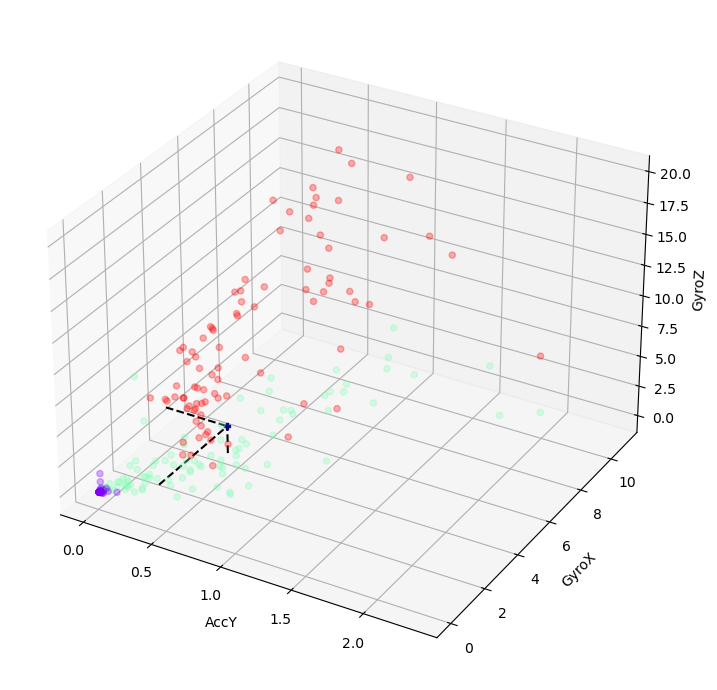
\includegraphics{Bericht_files/live-predict-plot.png}
\caption{live-predict-plot.png}
\end{figure}

Eine beispielhafte Ausgabe der Live-Prediction. Die Trainingsdaten sind
blasser mit kleineren Punkten dargestellt. Die aktuelle Prädiktion ist
mit einem tiefblauen Kreuz dargestellt.

    \hypertarget{analyse-der-qualituxe4t-der-klassifizierung-anhand-von-konfusions-matrizen}{%
\subsection*{2.11 Analyse der Qualität der Klassifizierung anhand von
Konfusions-Matrizen}\label{analyse-der-qualituxe4t-der-klassifizierung-anhand-von-konfusions-matrizen}}

    In diesem Abschnitt ist die Qualität der Klassifizierung anhand von
Confusions Matritzen visualisiert. Bei 100\% Accuracy wären nur die
Felder auf der Hauptdiagonale besetzt.

    \begin{tcolorbox}[breakable, size=fbox, boxrule=1pt, pad at break*=1mm,colback=cellbackground, colframe=cellborder]
\prompt{In}{incolor}{125}{\boxspacing}
\begin{Verbatim}[commandchars=\\\{\}]
\PY{k+kn}{import} \PY{n+nn}{seaborn} \PY{k}{as} \PY{n+nn}{sns}
\PY{k+kn}{import} \PY{n+nn}{pandas} \PY{k}{as} \PY{n+nn}{pd}

\PY{c+c1}{\PYZsh{} Funktion zur Erstellung einer Confusion Matrix}
\PY{k}{def} \PY{n+nf}{confusion\PYZus{}matrix}\PY{p}{(}\PY{n}{results}\PY{p}{,} \PY{n}{labels}\PY{p}{)}\PY{p}{:}
    \PY{n}{data} \PY{o}{=} \PY{p}{\PYZob{}}\PY{l+s+s1}{\PYZsq{}}\PY{l+s+s1}{y\PYZus{}Actual}\PY{l+s+s1}{\PYZsq{}}\PY{p}{:} \PY{n}{results}\PY{o}{.}\PY{n}{astype}\PY{p}{(}\PY{n}{np}\PY{o}{.}\PY{n}{uint8}\PY{p}{)}\PY{p}{,} \PY{l+s+s1}{\PYZsq{}}\PY{l+s+s1}{y\PYZus{}Predicted}\PY{l+s+s1}{\PYZsq{}}\PY{p}{:} \PY{n}{labels}\PY{p}{\PYZcb{}}
    \PY{n}{df} \PY{o}{=} \PY{n}{pd}\PY{o}{.}\PY{n}{DataFrame}\PY{p}{(}\PY{n}{data}\PY{p}{,} \PY{n}{columns}\PY{o}{=}\PY{p}{[}\PY{l+s+s1}{\PYZsq{}}\PY{l+s+s1}{y\PYZus{}Actual}\PY{l+s+s1}{\PYZsq{}}\PY{p}{,} \PY{l+s+s1}{\PYZsq{}}\PY{l+s+s1}{y\PYZus{}Predicted}\PY{l+s+s1}{\PYZsq{}}\PY{p}{]}\PY{p}{)}
    \PY{n}{cm} \PY{o}{=} \PY{n}{pd}\PY{o}{.}\PY{n}{crosstab}\PY{p}{(}\PY{n}{df}\PY{p}{[}\PY{l+s+s1}{\PYZsq{}}\PY{l+s+s1}{y\PYZus{}Actual}\PY{l+s+s1}{\PYZsq{}}\PY{p}{]}\PY{p}{,} \PY{n}{df}\PY{p}{[}\PY{l+s+s1}{\PYZsq{}}\PY{l+s+s1}{y\PYZus{}Predicted}\PY{l+s+s1}{\PYZsq{}}\PY{p}{]}\PY{p}{)}
    \PY{n}{cm} \PY{o}{=} \PY{n}{cm}\PY{o}{.}\PY{n}{astype}\PY{p}{(}\PY{n}{np}\PY{o}{.}\PY{n}{float32}\PY{p}{)} \PY{o}{/} \PY{n}{cm}\PY{o}{.}\PY{n}{sum}\PY{p}{(}\PY{n}{axis}\PY{o}{=}\PY{l+m+mi}{1}\PY{p}{)}\PY{o}{.}\PY{n}{values}\PY{p}{[}\PY{p}{:}\PY{p}{,} \PY{n}{np}\PY{o}{.}\PY{n}{newaxis}\PY{p}{]} \PY{o}{*} \PY{l+m+mf}{100.0}
    \PY{n}{sns}\PY{o}{.}\PY{n}{heatmap}\PY{p}{(}\PY{n}{cm}\PY{p}{,} \PY{n}{annot}\PY{o}{=}\PY{k+kc}{True}\PY{p}{,} \PY{n}{fmt}\PY{o}{=}\PY{l+s+s1}{\PYZsq{}}\PY{l+s+s1}{.1f}\PY{l+s+s1}{\PYZsq{}}\PY{p}{,} \PY{n}{annot\PYZus{}kws}\PY{o}{=}\PY{p}{\PYZob{}}\PY{l+s+s2}{\PYZdq{}}\PY{l+s+s2}{size}\PY{l+s+s2}{\PYZdq{}}\PY{p}{:} \PY{l+m+mi}{8}\PY{p}{\PYZcb{}}\PY{p}{)}
    \PY{n}{plt}\PY{o}{.}\PY{n}{title}\PY{p}{(}\PY{l+s+s1}{\PYZsq{}}\PY{l+s+s1}{Normalized Confusion Matrix in }\PY{l+s+s1}{\PYZpc{}}\PY{l+s+s1}{\PYZsq{}}\PY{p}{)}
    \PY{n}{plt}\PY{o}{.}\PY{n}{show}\PY{p}{(}\PY{p}{)}
\end{Verbatim}
\end{tcolorbox}

    Ausgabe der Confusion Matritzen, der Validierungs- und Trainingsdaten.

    \begin{tcolorbox}[breakable, size=fbox, boxrule=1pt, pad at break*=1mm,colback=cellbackground, colframe=cellborder]
\prompt{In}{incolor}{126}{\boxspacing}
\begin{Verbatim}[commandchars=\\\{\}]
\PY{c+c1}{\PYZsh{} Confusion Matritzen mit verarbeiteten Daten}

\PY{c+c1}{\PYZsh{} Ergebnis Trainingsdaten}
\PY{n}{confusion\PYZus{}matrix}\PY{p}{(}\PY{n}{y\PYZus{}predict}\PY{p}{,} \PY{p}{(}\PY{n}{data\PYZus{}scaled\PYZus{}df}\PY{p}{[}\PY{l+s+s1}{\PYZsq{}}\PY{l+s+s1}{class}\PY{l+s+s1}{\PYZsq{}}\PY{p}{]}\PY{p}{)}\PY{o}{.}\PY{n}{astype}\PY{p}{(}\PY{n+nb}{int}\PY{p}{)}\PY{o}{.}\PY{n}{values}\PY{p}{)}

\PY{c+c1}{\PYZsh{} Ergebnis Validierungsdaten}
\PY{n}{confusion\PYZus{}matrix}\PY{p}{(}\PY{n}{prediction}\PY{p}{,} \PY{n}{val\PYZus{}labels}\PY{o}{.}\PY{n}{astype}\PY{p}{(}\PY{n+nb}{int}\PY{p}{)}\PY{o}{.}\PY{n}{values}\PY{p}{)}
\end{Verbatim}
\end{tcolorbox}

    \begin{center}
    \adjustimage{max size={0.9\linewidth}{0.9\paperheight}}{Bericht_files/Bericht_68_0.png}
    \end{center}
    { \hspace*{\fill} \\}
    
    \begin{center}
    \adjustimage{max size={0.9\linewidth}{0.9\paperheight}}{Bericht_files/Bericht_68_1.png}
    \end{center}
    { \hspace*{\fill} \\}
    
    Die erste Confusion Matrix visualisiert die Ergebnisse der Accuracy auf
dem Validierungsdatensatz. Das numerische Ergebnis von 100\% Accuracy
deckt sich mit der Beobachtung, dass nur Felder der Hauptdiagonalen
besetzt sind und diese gleichzeitig 100\% Accuracy enthalten.

Die zweite Confusion Matrix visualisiert die Ergebnisse der Accuracy auf
dem Trainingsdatensatz. Es fällt auf, das die Klasse Ruhe am besten mit
100 \% korrekt klassifiziert wird. Dies ist plausibel, da sich die
Sensordaten hier deutlich von denen der anderen zwei Klassen
unterscheiden, indem sie nur eine kleine Standardabweichung aufweisen.
Die anderen beiden Klassen werden mit jeweils 96,9\% (Klasse 2) und
97,6\% korrekt klassifiziert. Zusammen ergeben die Klassenspezifischen
Accuracys die erwartete durchschnittliche Accuracy von knapp über 98\%.

    \hypertarget{fazit}{%
\subsection*{3 Fazit}\label{fazit}}

    In diesem Inkrement konnte das Vorgehen bei der korrekten
Vorverarbeitung von Daten, dem Trainieren eines k-NN-Klassifikators und
der Bewertung der Klassifizierungsergebnisse vertieft werden. Darüber
hinaus wurde deutlich wie Feature-Engineering anhand der Visualisierung
von Sensorpaaren durchgeführt werden kann. Desweiteren wurde deutlich,
dass die Weiterverarbeitung von Sensorrohdaten zu einer erheblichen
Verbesserung des Klassifizierungsergebnisses führen kann. Allein mit der
Standardabweichung als einzige Kenngröße konnte eine Accuracy von
mindestens 98\% erziehlt werden. Das Ergänzen von weiteren statistischen
Werten, wie dem Minimum, Maximum oder Zeitabhängigen Größen, wie
beispielsweise der Geschwindigkeit würden dieses Ergebnis vermutlich
noch verbessern.

    \hypertarget{anhang}{%
\subsection*{Anhang}\label{anhang}}

    \hypertarget{verwendetes-node-red-netzwerk}{%
\subsubsection*{Verwendetes
Node-Red-Netzwerk}\label{verwendetes-node-red-netzwerk}}

    \begin{figure}
\centering
\includegraphics{Bericht_files/nr-netzwerk.png}
\caption{nr-netzwerk.png}
\end{figure}

    Die Darstellung illustriert das Node-Red-Netzwerk, das für die Erfassung
des Datensatzes verwendet wird. Durch Aktivierung des blau
hervorgehobenen Insert-Bausteins (Header) kann der Kopfzeilen-Header des
CSV-Files manuell eingefügt werden. Der Zustand (State) kann mithilfe
des Insert-Bausteins (state) modifiziert werden. Hierfür ist vor der
Aktivierung des Bausteins der Zustand als Zahlenwert 1..3 im Payload
einzutragen, wobei 1 für Ruhe, 2 für Fernsteuerung und 3 für Transport
steht. Der Baustein ``state'' ist ausschließlich für die Datenerfassung
zu verwenden und besitzt bei einer Live-Klassifizierung keine Funktion.

    \hypertarget{ergebnisse-ohne-datenvorverarbeitung}{%
\subsection*{Ergebnisse ohne
Datenvorverarbeitung}\label{ergebnisse-ohne-datenvorverarbeitung}}

    Hier ist der Versuchsteil dokumentiert, bei dem auf eine
Datenvorverarbeitung verzichtet wird.

    \begin{tcolorbox}[breakable, size=fbox, boxrule=1pt, pad at break*=1mm,colback=cellbackground, colframe=cellborder]
\prompt{In}{incolor}{58}{\boxspacing}
\begin{Verbatim}[commandchars=\\\{\}]
\PY{c+c1}{\PYZsh{}from itertools import combinations}
\PY{k+kn}{import} \PY{n+nn}{pandas} \PY{k}{as} \PY{n+nn}{pd}
\PY{k+kn}{import} \PY{n+nn}{matplotlib}\PY{n+nn}{.}\PY{n+nn}{pyplot} \PY{k}{as} \PY{n+nn}{plt}

\PY{c+c1}{\PYZsh{} Skalierte Werte in einem neuen DataFrame mit den ursprünglichen Spaltennamen}
\PY{n}{data\PYZus{}scaled\PYZus{}df} \PY{o}{=} \PY{n}{pd}\PY{o}{.}\PY{n}{DataFrame}\PY{p}{(}\PY{n}{data\PYZus{}scaled}\PY{p}{,} \PY{n}{columns}\PY{o}{=}\PY{n}{data}\PY{o}{.}\PY{n}{columns}\PY{p}{)}

\PY{c+c1}{\PYZsh{} Erstelle eine temporäre Spalte \PYZsq{}class\PYZsq{} basierend auf One\PYZhy{}Hot\PYZhy{}Encoding}
\PY{n}{data\PYZus{}scaled\PYZus{}df}\PY{p}{[}\PY{l+s+s1}{\PYZsq{}}\PY{l+s+s1}{class}\PY{l+s+s1}{\PYZsq{}}\PY{p}{]} \PY{o}{=} \PY{n}{data\PYZus{}scaled\PYZus{}df}\PY{o}{.}\PY{n}{apply}\PY{p}{(}\PY{k}{lambda} \PY{n}{row}\PY{p}{:} \PY{l+m+mi}{1} \PY{k}{if} \PY{n}{row}\PY{p}{[}\PY{l+s+s1}{\PYZsq{}}\PY{l+s+s1}{RuheState}\PY{l+s+s1}{\PYZsq{}}\PY{p}{]} \PY{o}{==} \PY{l+m+mi}{1} \PY{k}{else} \PY{p}{(}\PY{l+m+mi}{2} \PY{k}{if} \PY{n}{row}\PY{p}{[}\PY{l+s+s1}{\PYZsq{}}\PY{l+s+s1}{FernstState}\PY{l+s+s1}{\PYZsq{}}\PY{p}{]} \PY{o}{==} \PY{l+m+mi}{1} \PY{k}{else} \PY{l+m+mi}{3}\PY{p}{)}\PY{p}{,} \PY{n}{axis}\PY{o}{=}\PY{l+m+mi}{1}\PY{p}{)}

\PY{c+c1}{\PYZsh{} Liste der ausgewählten Sensoren}
\PY{n}{selected\PYZus{}sensors} \PY{o}{=} \PY{p}{[}\PY{l+s+s1}{\PYZsq{}}\PY{l+s+s1}{AccX}\PY{l+s+s1}{\PYZsq{}}\PY{p}{,} \PY{l+s+s1}{\PYZsq{}}\PY{l+s+s1}{AccY}\PY{l+s+s1}{\PYZsq{}}\PY{p}{,} \PY{l+s+s1}{\PYZsq{}}\PY{l+s+s1}{AccZ}\PY{l+s+s1}{\PYZsq{}}\PY{p}{,} \PY{l+s+s1}{\PYZsq{}}\PY{l+s+s1}{GyroY}\PY{l+s+s1}{\PYZsq{}}\PY{p}{]}

\PY{c+c1}{\PYZsh{} Erstelle alle möglichen Kombinationen von Label\PYZhy{}Paaren für die ausgewählten Sensoren}
\PY{n}{label\PYZus{}pairs} \PY{o}{=} \PY{n+nb}{list}\PY{p}{(}\PY{n}{combinations}\PY{p}{(}\PY{n}{selected\PYZus{}sensors}\PY{p}{,} \PY{l+m+mi}{2}\PY{p}{)}\PY{p}{)}
\PY{n+nb}{print}\PY{p}{(}\PY{n+nb}{len}\PY{p}{(}\PY{n}{label\PYZus{}pairs}\PY{p}{)}\PY{p}{)}

\PY{c+c1}{\PYZsh{} Anzahl der Zeilen und Spalten für die Subplots}
\PY{n}{num\PYZus{}rows} \PY{o}{=} \PY{l+m+mi}{2}  \PY{c+c1}{\PYZsh{} Festgelegte Anzahl der Zeilen basierend auf der Anzahl der ausgewählten Sensoren}
\PY{n}{num\PYZus{}cols} \PY{o}{=} \PY{n+nb}{len}\PY{p}{(}\PY{n}{selected\PYZus{}sensors}\PY{p}{)} \PY{o}{\PYZhy{}} \PY{l+m+mi}{1}  \PY{c+c1}{\PYZsh{} Eine Spalte weniger als die Anzahl der ausgewählten Sensoren}

\PY{c+c1}{\PYZsh{} Erstelle Subplots}
\PY{n}{fig}\PY{p}{,} \PY{n}{axs} \PY{o}{=} \PY{n}{plt}\PY{o}{.}\PY{n}{subplots}\PY{p}{(}\PY{n}{num\PYZus{}rows}\PY{p}{,} \PY{n}{num\PYZus{}cols}\PY{p}{,} \PY{n}{figsize}\PY{o}{=}\PY{p}{(}\PY{l+m+mi}{15}\PY{p}{,} \PY{l+m+mi}{8}\PY{p}{)}\PY{p}{)}

\PY{c+c1}{\PYZsh{} Iteriere durch Label\PYZhy{}Paare und erstelle Scatterplots}
\PY{k}{for} \PY{n}{i} \PY{o+ow}{in} \PY{n+nb}{range}\PY{p}{(}\PY{n}{num\PYZus{}rows}\PY{p}{)}\PY{p}{:}
    \PY{k}{for} \PY{n}{j} \PY{o+ow}{in} \PY{n+nb}{range}\PY{p}{(}\PY{n}{num\PYZus{}cols}\PY{p}{)}\PY{p}{:}
        \PY{n}{label\PYZus{}pair} \PY{o}{=} \PY{n}{label\PYZus{}pairs}\PY{p}{[}\PY{n}{i} \PY{o}{*} \PY{n}{num\PYZus{}cols} \PY{o}{+} \PY{n}{j}\PY{p}{]}
        \PY{n}{axs}\PY{p}{[}\PY{n}{i}\PY{p}{,} \PY{n}{j}\PY{p}{]}\PY{o}{.}\PY{n}{scatter}\PY{p}{(}\PY{n}{data\PYZus{}scaled\PYZus{}df}\PY{p}{[}\PY{n}{label\PYZus{}pair}\PY{p}{[}\PY{l+m+mi}{0}\PY{p}{]}\PY{p}{]}\PY{p}{,} \PY{n}{data\PYZus{}scaled\PYZus{}df}\PY{p}{[}\PY{n}{label\PYZus{}pair}\PY{p}{[}\PY{l+m+mi}{1}\PY{p}{]}\PY{p}{]}\PY{p}{,} \PY{n}{alpha}\PY{o}{=}\PY{l+m+mf}{0.1}\PY{p}{,} \PY{n}{c}\PY{o}{=}\PY{n}{data\PYZus{}scaled\PYZus{}df}\PY{p}{[}\PY{l+s+s1}{\PYZsq{}}\PY{l+s+s1}{class}\PY{l+s+s1}{\PYZsq{}}\PY{p}{]}\PY{p}{,} \PY{n}{cmap}\PY{o}{=}\PY{n}{plt}\PY{o}{.}\PY{n}{get\PYZus{}cmap}\PY{p}{(}\PY{l+s+s1}{\PYZsq{}}\PY{l+s+s1}{jet}\PY{l+s+s1}{\PYZsq{}}\PY{p}{)}\PY{p}{)}
        \PY{n}{axs}\PY{p}{[}\PY{n}{i}\PY{p}{,} \PY{n}{j}\PY{p}{]}\PY{o}{.}\PY{n}{set\PYZus{}title}\PY{p}{(}\PY{l+s+sa}{f}\PY{l+s+s1}{\PYZsq{}}\PY{l+s+s1}{Skalierte Werte \PYZhy{} }\PY{l+s+si}{\PYZob{}}\PY{n}{label\PYZus{}pair}\PY{p}{[}\PY{l+m+mi}{0}\PY{p}{]}\PY{l+s+si}{\PYZcb{}}\PY{l+s+s1}{ vs. }\PY{l+s+si}{\PYZob{}}\PY{n}{label\PYZus{}pair}\PY{p}{[}\PY{l+m+mi}{1}\PY{p}{]}\PY{l+s+si}{\PYZcb{}}\PY{l+s+s1}{\PYZsq{}}\PY{p}{)}

\PY{c+c1}{\PYZsh{} Verbessere das Layout}
\PY{n}{plt}\PY{o}{.}\PY{n}{tight\PYZus{}layout}\PY{p}{(}\PY{p}{)}
\PY{n}{plt}\PY{o}{.}\PY{n}{show}\PY{p}{(}\PY{p}{)}
\end{Verbatim}
\end{tcolorbox}

    \begin{Verbatim}[commandchars=\\\{\}]
6
    \end{Verbatim}

    \begin{center}
    \adjustimage{max size={0.9\linewidth}{0.9\paperheight}}{Bericht_files/Bericht_78_1.png}
    \end{center}
    { \hspace*{\fill} \\}
    
    \hypertarget{visualisierung-der-gegenuxfcberstellung-der-ausgewuxe4hlten-sensoren}{%
\subsubsection*{Visualisierung, der Gegenüberstellung, der ausgewählten
Sensoren}\label{visualisierung-der-gegenuxfcberstellung-der-ausgewuxe4hlten-sensoren}}

    Aus den Sensoren wurden die vier vielversprechensten skalierten Features
in 2D-Plots visualisiert. Die sich ergebenden Cluster sind sehr
ausgeprägt und es ist zu erwarten, dass die Kombination dieser Features
im multidimensionalen Merkmalsraum zu überlagerungsfreien Clustern
führt.

    \begin{figure}
\centering
\includegraphics{Bericht_files/image.png}
\caption{image.png}
\end{figure}

    \hypertarget{extraktion-der-features}{%
\subsubsection*{Extraktion der Features}\label{extraktion-der-features}}

    \begin{tcolorbox}[breakable, size=fbox, boxrule=1pt, pad at break*=1mm,colback=cellbackground, colframe=cellborder]
\prompt{In}{incolor}{69}{\boxspacing}
\begin{Verbatim}[commandchars=\\\{\}]
\PY{c+c1}{\PYZsh{} Extrahiere die Labels}
\PY{n}{train\PYZus{}labels} \PY{o}{=} \PY{n}{data\PYZus{}scaled\PYZus{}df}\PY{p}{[}\PY{l+s+s1}{\PYZsq{}}\PY{l+s+s1}{class}\PY{l+s+s1}{\PYZsq{}}\PY{p}{]}

\PY{n}{val\PYZus{}labels} \PY{o}{=} \PY{n}{pd}\PY{o}{.}\PY{n}{DataFrame}\PY{p}{(}\PY{n}{columns}\PY{o}{=}\PY{p}{[}\PY{l+s+s1}{\PYZsq{}}\PY{l+s+s1}{class}\PY{l+s+s1}{\PYZsq{}}\PY{p}{]}\PY{p}{)}
\PY{n}{val\PYZus{}labels} \PY{o}{=} \PY{n}{val}\PY{o}{.}\PY{n}{apply}\PY{p}{(}\PY{k}{lambda} \PY{n}{row}\PY{p}{:} \PY{l+m+mi}{1} \PY{k}{if} \PY{n}{row}\PY{p}{[}\PY{l+s+s1}{\PYZsq{}}\PY{l+s+s1}{RuheState}\PY{l+s+s1}{\PYZsq{}}\PY{p}{]} \PY{o}{==} \PY{l+m+mi}{1} \PY{k}{else} \PY{p}{(}\PY{l+m+mi}{2} \PY{k}{if} \PY{n}{row}\PY{p}{[}\PY{l+s+s1}{\PYZsq{}}\PY{l+s+s1}{FernstState}\PY{l+s+s1}{\PYZsq{}}\PY{p}{]} \PY{o}{==} \PY{l+m+mi}{1} \PY{k}{else} \PY{l+m+mi}{3}\PY{p}{)}\PY{p}{,} \PY{n}{axis}\PY{o}{=}\PY{l+m+mi}{1}\PY{p}{)}


\PY{c+c1}{\PYZsh{} Extrahiere die Features für die ausgewählten Sensoren}
\PY{n}{train\PYZus{}features} \PY{o}{=} \PY{n}{data\PYZus{}scaled\PYZus{}df}\PY{p}{[}\PY{n}{selected\PYZus{}sensors}\PY{p}{]}
\PY{n}{val\PYZus{}features} \PY{o}{=} \PY{n}{val}\PY{p}{[}\PY{n}{selected\PYZus{}sensors}\PY{p}{]}
\end{Verbatim}
\end{tcolorbox}

    \hypertarget{training-des-k-nn-klassifikators-mit-den-ausgewuxe4hlten-features}{%
\subsubsection*{Training des k-NN-Klassifikators mit den ausgewählten
Features}\label{training-des-k-nn-klassifikators-mit-den-ausgewuxe4hlten-features}}

    \begin{tcolorbox}[breakable, size=fbox, boxrule=1pt, pad at break*=1mm,colback=cellbackground, colframe=cellborder]
\prompt{In}{incolor}{71}{\boxspacing}
\begin{Verbatim}[commandchars=\\\{\}]
\PY{k+kn}{from} \PY{n+nn}{sklearn} \PY{k+kn}{import} \PY{n}{neighbors}
\PY{k+kn}{import} \PY{n+nn}{numpy} \PY{k}{as} \PY{n+nn}{np}

\PY{c+c1}{\PYZsh{} K\PYZhy{}NN Klassifikator}
\PY{n}{k} \PY{o}{=} \PY{l+m+mi}{5}
\PY{n}{clf} \PY{o}{=} \PY{n}{neighbors}\PY{o}{.}\PY{n}{KNeighborsClassifier}\PY{p}{(}\PY{n}{n\PYZus{}neighbors}\PY{o}{=}\PY{n}{k}\PY{p}{)}

\PY{c+c1}{\PYZsh{} Training des Klassifikators}
\PY{n}{clf}\PY{o}{.}\PY{n}{fit}\PY{p}{(}\PY{n}{train\PYZus{}features}\PY{p}{,} \PY{n}{train\PYZus{}labels}\PY{p}{)}
\end{Verbatim}
\end{tcolorbox}

            \begin{tcolorbox}[breakable, size=fbox, boxrule=.5pt, pad at break*=1mm, opacityfill=0]
\prompt{Out}{outcolor}{71}{\boxspacing}
\begin{Verbatim}[commandchars=\\\{\}]
KNeighborsClassifier()
\end{Verbatim}
\end{tcolorbox}
        
    \hypertarget{klassifizierung-des-trainings--und-valisierungsdatensatzes}{%
\subsubsection*{Klassifizierung des Trainings- und
Valisierungsdatensatzes}\label{klassifizierung-des-trainings--und-valisierungsdatensatzes}}

    \begin{tcolorbox}[breakable, size=fbox, boxrule=1pt, pad at break*=1mm,colback=cellbackground, colframe=cellborder]
\prompt{In}{incolor}{72}{\boxspacing}
\begin{Verbatim}[commandchars=\\\{\}]
\PY{c+c1}{\PYZsh{} Prediction für Trainingsdaten}
\PY{n}{train\PYZus{}prediction} \PY{o}{=} \PY{n}{clf}\PY{o}{.}\PY{n}{predict}\PY{p}{(}\PY{n}{train\PYZus{}features}\PY{p}{)}

\PY{c+c1}{\PYZsh{} Prediction für Validierungsdaten}
\PY{n}{val\PYZus{}prediction} \PY{o}{=} \PY{n}{clf}\PY{o}{.}\PY{n}{predict}\PY{p}{(}\PY{n}{val\PYZus{}features}\PY{p}{)}
\end{Verbatim}
\end{tcolorbox}

    \hypertarget{berechnung-der-trainings--und-validierungs-accuracy}{%
\subsubsection*{Berechnung der Trainings- und Validierungs
Accuracy}\label{berechnung-der-trainings--und-validierungs-accuracy}}

    \begin{tcolorbox}[breakable, size=fbox, boxrule=1pt, pad at break*=1mm,colback=cellbackground, colframe=cellborder]
\prompt{In}{incolor}{73}{\boxspacing}
\begin{Verbatim}[commandchars=\\\{\}]
\PY{c+c1}{\PYZsh{} Berechne Trainingsgenauigkeit}
\PY{n}{train\PYZus{}acc} \PY{o}{=} \PY{n}{np}\PY{o}{.}\PY{n}{mean}\PY{p}{(}\PY{n}{train\PYZus{}prediction} \PY{o}{==} \PY{n}{train\PYZus{}labels}\PY{o}{.}\PY{n}{astype}\PY{p}{(}\PY{n+nb}{int}\PY{p}{)}\PY{o}{.}\PY{n}{values}\PY{p}{)}
\PY{n+nb}{print}\PY{p}{(}\PY{l+s+sa}{f}\PY{l+s+s2}{\PYZdq{}}\PY{l+s+s2}{Train Accuracy: }\PY{l+s+si}{\PYZob{}}\PY{n}{train\PYZus{}acc}\PY{l+s+si}{\PYZcb{}}\PY{l+s+s2}{\PYZdq{}}\PY{p}{)}

\PY{c+c1}{\PYZsh{} Berechne Validierungsgenauigkeit}
\PY{n}{val\PYZus{}acc} \PY{o}{=} \PY{n}{np}\PY{o}{.}\PY{n}{mean}\PY{p}{(}\PY{n}{val\PYZus{}prediction} \PY{o}{==} \PY{n}{val\PYZus{}labels}\PY{o}{.}\PY{n}{astype}\PY{p}{(}\PY{n+nb}{int}\PY{p}{)}\PY{o}{.}\PY{n}{values}\PY{p}{)}
\PY{n+nb}{print}\PY{p}{(}\PY{l+s+sa}{f}\PY{l+s+s2}{\PYZdq{}}\PY{l+s+s2}{Validation Accuracy: }\PY{l+s+si}{\PYZob{}}\PY{n}{val\PYZus{}acc}\PY{l+s+si}{\PYZcb{}}\PY{l+s+s2}{\PYZdq{}}\PY{p}{)}
\end{Verbatim}
\end{tcolorbox}

    \begin{Verbatim}[commandchars=\\\{\}]
Train Accuracy: 0.9428606237816765
Validation Accuracy: 0.9287280701754386
    \end{Verbatim}

    \hypertarget{ergebnisse-der-klassifizierung}{%
\subsubsection*{Ergebnisse der
Klassifizierung}\label{ergebnisse-der-klassifizierung}}

    Train Accuracy: 0.9428606237816765

Validation Accuracy: 0.9287280701754386

    \hypertarget{confusion-matrix}{%
\subsubsection*{Confusion Matrix}\label{confusion-matrix}}

    \begin{tcolorbox}[breakable, size=fbox, boxrule=1pt, pad at break*=1mm,colback=cellbackground, colframe=cellborder]
\prompt{In}{incolor}{76}{\boxspacing}
\begin{Verbatim}[commandchars=\\\{\}]
\PY{c+c1}{\PYZsh{} Confusion Matrizen ohne Datenvorverarbeitung}

\PY{c+c1}{\PYZsh{} Ergebnis Validierungsdaten}
\PY{n}{confusion\PYZus{}matrix}\PY{p}{(}\PY{n}{val\PYZus{}prediction}\PY{p}{,} \PY{n}{val\PYZus{}labels}\PY{o}{.}\PY{n}{astype}\PY{p}{(}\PY{n+nb}{int}\PY{p}{)}\PY{o}{.}\PY{n}{values}\PY{p}{)}

\PY{c+c1}{\PYZsh{} Ergebnis Trainingsdaten}
\PY{n}{confusion\PYZus{}matrix}\PY{p}{(}\PY{n}{train\PYZus{}prediction}\PY{p}{,} \PY{n}{train\PYZus{}labels}\PY{o}{.}\PY{n}{astype}\PY{p}{(}\PY{n+nb}{int}\PY{p}{)}\PY{o}{.}\PY{n}{values}\PY{p}{)}
\end{Verbatim}
\end{tcolorbox}

    \begin{center}
    \adjustimage{max size={0.9\linewidth}{0.9\paperheight}}{Bericht_files/Bericht_93_0.png}
    \end{center}
    { \hspace*{\fill} \\}
    
    \begin{center}
    \adjustimage{max size={0.9\linewidth}{0.9\paperheight}}{Bericht_files/Bericht_93_1.png}
    \end{center}
    { \hspace*{\fill} \\}
    
    Sowohl bei den Trainingsdaten, als auch bei den Validierungsdaten hat
der k-NN-Klassifikator Probleme den Unterschied zwischen Fernsteuerung
und Transport korrekt zu erkennen. Diese Falschklasssifizierung zwischen
Fernsteuerung und Transport beeinflusst das Gesamtergebnis der
Klassifizierungsgenauigkeit am deutlichsten. Mit fast 8\%
Falschklassifizierung auf Validierungsdaten und knapp 2\% auf
Trainingsdaten wurde wiederholt Transport als Fernsteuerung
Klassifiziert.

    \hypertarget{fazit}{%
\subsubsection*{Fazit}\label{fazit}}

    Mit 94\% Accuracy auf Trainingsdaten und 92\% Accuracy auf
Validierungsdaten kann bereits eine sehr hohe
Klassifizierungsgenauigkeit bei unverarbeiteten Datensätzen erreicht
werden. Die Klassifizierung mit unverarbeiteten Daten ergibt eine
geringere Accuracy auf Validierungsdaten, als auf Trainingsdaten. Das
zeigt, dass der k-NN-Klassifikator nicht so gut generalisieren kann.
Dabei beträgt die Abweichung zwischen Trainings- und Validation-Accuracy
nur ca. 2 Prozentpunkte.


    % Add a bibliography block to the postdoc
    
    
    
\end{document}
